\documentclass[a4paper,12pt]{report}

%% Language and font encodings
\usepackage[english]{babel}
\usepackage[utf8]{inputenc}
\usepackage[T1]{fontenc}

%% Sets page size and margins according to Bonn University guidelines
\usepackage[a4paper,top=2cm,bottom=2cm,left=3cm,right=2cm]{geometry}

%% Font settings - Times New Roman or similar (as per guidelines)
\usepackage{times} % Times font
\usepackage{mathptmx} % Times font with math support

%% Section formatting
\usepackage{titlesec}

% Traditional academic chapter title style
\titleformat{\chapter}[display]
  {\normalfont\Large\bfseries}
  {}
  {0pt}
  {\thispagestyle{empty}%
   \vspace*{-20pt}%
   \begin{flushright}
     % Elegant, academic chapter number
     \begin{tikzpicture}[remember picture, overlay]
       \node[text=black!12, font=\fontsize{80}{80}\selectfont] {\thechapter};
     \end{tikzpicture}
   \end{flushright}
   \vspace{-60pt}
   % Simple, elegant single line
   \rule{\textwidth}{0.6pt}\\
   \vspace*{15pt}
   \raggedright\LARGE\scshape}
  [\vspace{-0.8cm}]
\titlespacing*{\chapter}{0pt}{0pt}{40pt}

% Elegant section formatting
\titleformat{\section}
  {\normalfont\Large\bfseries\scshape}
  {}
  {0pt}
  {\thesection\quad}
\titlespacing*{\section}{0pt}{3.5ex plus 1ex minus .2ex}{1.5ex plus .2ex}

% Make subsections italic and elegant
\titleformat{\subsection}
  {\normalfont\large\bfseries\itshape}
  {\thesubsection}
  {1em}
  {}
\titlespacing*{\subsection}{0pt}{3ex plus 1ex minus .2ex}{1.5ex plus .2ex}

%% Line spacing 1.5 as required
\usepackage{setspace}
\onehalfspacing

%% Useful packages
\usepackage{amsmath}
\usepackage{amssymb}
\usepackage{bm}         % For bold symbols
\usepackage{graphicx}
\usepackage{float}      % For [H] figure placement
\usepackage{booktabs}
\usepackage{tabu}
\usepackage{enumitem}
\usepackage[table,dvipsnames]{xcolor}  % Added dvipsnames option for more color choices
\usepackage{array}
\usepackage{multirow}
\usepackage{amsthm}
\usepackage{bbm}        % Blackboard math symbols (for indicator function)
\usepackage[toc]{appendix}
\usepackage{subcaption}

% Choose either algorithm2e OR algorithmicx, not both
\usepackage{algorithm}
\usepackage{algorithmicx}
\usepackage{algpseudocode}

% For adjusting margins of specific sections
\usepackage{changepage}

% Bibliography
\usepackage[natbibapa]{apacite}

% Todo notes
\usepackage[colorinlistoftodos]{todonotes}

% Page numbering configuration
\usepackage{fancyhdr}
\pagestyle{fancy}
\fancyhf{}
\fancyfoot[C]{\thepage}
\renewcommand{\headrulewidth}{0pt}

% Hyperref should be last
\usepackage[colorlinks=true, allcolors=blue]{hyperref}

% Allow floating content to be placed more liberally
\renewcommand{\floatpagefraction}{.9}
\renewcommand{\textfraction}{.1}
\renewcommand{\topfraction}{0.9}
\renewcommand{\bottomfraction}{.9}

% Appendix formatting
\makeatletter
\let\old@chapter\@chapter
\def\@chapter[#1]#2{\old@chapter[{#1}]{#2}}
\makeatother

% Math operators
\DeclareMathOperator*{\argmax}{arg\,max}
\DeclareMathOperator*{\argmin}{arg\,min}

% Custom theorem environments
\newtheorem{theorem}{Theorem}
\newtheorem{proposition}{Proposition}
\newtheorem{lemma}{Lemma}
\newtheorem{corollary}{Corollary}
\newtheorem{definition}{Definition}
\newtheorem{assumption}{Assumption}
\newtheorem{remark}{Remark}

% Define indicator function notation
\newcommand{\ind}[1]{\mathbbm{1}_{#1}}

\begin{document}

% Cover sheet as per Bonn University guidelines
\begin{titlepage}
\begin{center}
\vspace*{2cm}

{\Large \textbf{Social Learning via\\[0.25cm]Multi-Agent Deep Reinforcement Learning}}\\[6cm]

Master Thesis Presented to the\\
Department of Economics at the\\
Rheinische Friedrich-Wilhelms-Universität Bonn\\[1cm]

In Partial Fulfillment of the Requirements for the Degree of\\
Master of Science (M.Sc.)\\[4cm]

Supervisor: Prof. Dr. Florian Brandl\\[2cm]

Submitted in June, 2025 by:\\
Ege Can Doğaroğlu\\
Matriculation Number: 3464688

\end{center}
\end{titlepage}

% Set page numbering to 'gobble' (no numbers) for front matter
\pagenumbering{gobble}

% Abstract
\begin{abstract}
\begin{adjustwidth}{2cm}{2cm}
This thesis bridges economic social learning theory and multi-agent reinforcement learning by developing Partially Observable Active Markov Games (POAMGs) and the POLARIS algorithm. Our framework addresses fundamental challenges in modeling adaptive behavior under partial observability, where agents must simultaneously learn about uncertain environments and evolving strategies of others. We extend Active Markov Games to partially observable settings, derive theoretical convergence results, and develop a practical algorithm combining Transformer-based belief processing, Graph Neural Networks with attention mechanisms, and reinforcement learning optimization. Applied to strategic experimentation and learning without experimentation scenarios, our approach reveals dynamic role assignment as a robust organizing principle where agents naturally differentiate into complementary roles enhancing collective information processing. We find that free-riding behavior does not lead to uniform inefficiencies—for some agents, performance in larger networks exceeds autarky levels. Our two-staged analysis methodology addresses computational challenges like catastrophic forgetting while providing systematic approaches for extracting insights from multi-agent learning dynamics. The framework contributes theoretical foundations to multi-agent reinforcement learning and computational tools to economic theory, demonstrating how interdisciplinary approaches can illuminate complex social learning phenomena neither field could address alone.
\end{adjustwidth}
\end{abstract}

% Table of contents
\tableofcontents
\newpage

% Optional - include if you have abbreviations, tables, or figures to list
%\listoffigures
%\listoftables
%\newpage

% Page numbering starts here with Arabic numerals
\chapter{Introduction}
\pagenumbering{arabic}
\setcounter{page}{1}
The study of how individuals and groups learn from each other's actions and experiences has been a central focus in economic theory for decades. From the seminal contributions on information cascades by \citet{banerjee1992simple} and \citet{bikhchandani1992theory} to more recent explorations of learning in networks \citep{acemoglu2011bayesian, golub2010naive}, economic research has sought to understand how social interactions shape beliefs, decisions, and collective outcomes. Traditional economic models have provided valuable insights into phenomena such as herding behavior, where individuals rationally ignore their private information to follow the observed actions of predecessors. However, these models often rely on simplified assumptions about agents' behavior and reasoning processes, frequently restricting analysis to one-shot sequential decisions or steady-state equilibria rather than capturing the rich dynamics of repeated interactions where agents continuously adapt their strategies based on others' evolving behaviors.

Meanwhile, the field of multi-agent reinforcement learning (MARL) has experienced remarkable progress in developing algorithms that enable autonomous agents to learn effective strategies in complex, interactive environments. Recent advances in reinforcement learning have demonstrated impressive capabilities in strategic games \citep{silver2016mastering}, cooperative problem-solving \citep{baker2020emergentreciprocityteamformation}, and competitive scenarios \citep{openai2019dota2largescale}.  MARL offers powerful tools for modeling adaptive behavior in non-stationary environments where agents must continuously revise their strategies in response to others' changing behaviors. However, much of this work has focused on engineering objectives rather than modeling realistic human learning processes, limiting its applicability to fundamental questions in economic theory. Additionally, many MARL approaches struggle with the challenge of partial observability—a defining feature of social learning contexts where agents cannot directly observe others' private information or belief states.

This thesis bridges these domains by introducing a novel framework that integrates economic social learning theory with multi-agent reinforcement learning under partial observability. Our approach models social learning as a dynamic process where agents with limited information strategically adapt their behaviors while simultaneously learning about their environment and other agents' strategies. Through the development of Partially Observable Active Markov Games (POAMGs) and the POLARIS algorithm, we demonstrate how computational approaches can complement traditional economic theory while revealing new insights into complex social learning dynamics, particularly the emergence of dynamic role assignment as a fundamental organizing principle of multi-agent learning systems.

The first challenge concerns non-stationarity and strategic adaptation. Traditional economic models of social learning typically assume that agents follow fixed, myopic decision rules or Bayesian updating procedures that do not fully account for strategic adaptation over time. When agents repeatedly interact and observe each other's actions, however, they may adjust their strategies in anticipation of others' learning, creating a complex web of interdependent adaptation that fundamentally alters collective learning dynamics. This non-stationarity—where the effective environment an agent faces changes as other agents learn—represents a central challenge that requires new modeling approaches. Standard MARL algorithms often treat this non-stationarity as a technical obstacle to convergence rather than an intrinsic feature of multi-agent systems that agents should explicitly reason about and strategically exploit.

The second challenge involves partial observability, which pervades social learning contexts. In most real-world settings, agents cannot directly observe others' private information, beliefs, or decision processes. Instead, they must infer these hidden states from observable actions and outcomes. This partial observability compounds the complexity of strategic interaction, as agents must simultaneously learn about the underlying state of the world and about the belief formation processes of others. Economic models have often simplified this challenge through strong assumptions about common knowledge or by focusing on one-shot sequential decisions rather than repeated interactions. Similarly, many MARL approaches assume full observability of the state or treat partial observability as a technical challenge to be addressed through belief state tracking, without fully incorporating its strategic implications.

The third challenge concerns long-term strategic considerations in social learning. Agents often face a tension between immediate payoffs and long-term information generation. They may sometimes choose actions that appear suboptimal in the short term to influence the learning trajectories of others or to generate valuable information for future periods. For instance, in strategic experimentation contexts, agents might incur costs to explore unknown options, knowing that the resulting information will benefit both themselves and others in the future. Capturing these farsighted strategic considerations requires models that explicitly account for how current actions shape the future evolution of others' beliefs and behaviors—a capability that neither traditional economic models nor standard MARL algorithms fully provide.

To address these challenges, this thesis makes four interconnected contributions that advance both economic theory and multi-agent reinforcement learning. First, we develop Partially Observable Active Markov Games (POAMGs)—a novel formalism that extends the Active Markov Game framework introduced by \citet{kim2022influencing} to partially observable settings. Unlike standard reinforcement learning frameworks that treat non-stationarity as a challenge to be mitigated, POAMGs incorporate policy evolution as an integral part of the environment dynamics, allowing agents to reason about and strategically influence this evolution process. POAMGs explicitly model how agents' policies evolve over time based on observations and interactions, while accounting for the fundamental constraints imposed by partial observability.

Second, we provide a thorough theoretical analysis of convergence and equilibrium properties in POAMGs. We establish conditions under which the joint process of states, beliefs, and policy parameters converges to a unique stochastically stable distribution, ensuring that our models have well-defined limiting behavior despite the inherent non-stationarity of multi-agent learning. We derive policy gradient theorems for average and discounted reward objectives and extend our framework to continuous-time dynamics through stochastic differential equations. Critically, we reveal how game-theoretic equilibrium concepts relate to active equilibrium when agents account for others' learning, illuminating the fundamental tension between theoretical ex ante strategies and the ex post strategies that emerge through reinforcement learning.

Third, we introduce POLARIS (Partially Observable Learning with Active Reinforcement In Social environments), combining belief processing through Transformer models, variational inference learning with Graph Neural Networks (GNNs), and reinforcement learning optimization. Our implementation incorporates GNNs with temporal and spatial attention mechanisms that capture network topology and temporal dependencies, enabling agents to develop sophisticated strategies accounting for both environmental partial observability and strategic adaptation. POLARIS addresses the critical challenge of catastrophic forgetting through an ex-post analysis methodology that provides systematic approaches for extracting insights from multi-agent learning dynamics despite agents' inability to maintain stable policies across all states.

Fourth, we validate our framework through strategic experimentation and learning without experimentation applications, building on the models of \citet{bolton1999strategic}, \citet{keller2020undiscounted}, \citet{huang2024learning}, and \citet{brandl2024}. Our analysis demonstrates dynamic role assignment as a robust organizing principle, where agents naturally differentiate into complementary roles enhancing collective information processing. Contrary to theoretical predictions about free-riding inefficiencies, we show that performance of some agents in larger networks substantially exceeds autarky levels, revealing opportunities for more realistic behavioral models that account for computational agents' learning dynamics.

A key methodological innovation is our discretization approach for continuous-time economic models, which treats Lévy processes through Euler-Maruyama schemes and maps continuous decisions to discrete action probabilities. This provides computational implementation templates while preserving essential incentive structures from theoretical models. We construct observed reward functions that enable reinforcement learning without direct reward signals and develop specialized transformer loss functions for Lévy process observations. Our theoretically grounded off-equilibrium asymmetric analysis methods move beyond symmetric equilibria analysis, allowing heterogeneous agent behaviors and asymmetric strategy convergence—capabilities essential for understanding real-world social learning dynamics.

The insights gained advance theoretical knowledge and inform the design of platforms and institutions that facilitate efficient collective learning. Our finding that dynamic role assignment emerges as a natural organizing principle suggests that effective social learning systems develop specialized roles enhancing collective information processing, providing guidance for platform design and institutional arrangements in financial markets, organizational learning, online social networks, and collaborative scientific endeavors. By demonstrating the value of MARL techniques for addressing classical questions in economic theory while revealing computational challenges like catastrophic forgetting, we contribute to both fields and encourage further cross-disciplinary work leveraging complementary insights from these rich intellectual traditions.

The remainder of this thesis is organized as follows: Chapter 2 reviews the relevant literature on social learning in economic theory and multi-agent reinforcement learning, emphasizing the complementary strengths and limitations of these approaches and identifying opportunities for cross-fertilization. Chapter 3 introduces our theoretical framework, developing the formalism of Partially Observable Active Markov Games and deriving key results on convergence, policy gradients, and equilibrium concepts, as well as presenting the POLARIS algorithm, detailing its components, implementation considerations, and theoretical justifications. Chapter 4 applies our framework to strategic experimentation and learning without experimentation, demonstrating how POLARIS captures sophisticated social learning dynamics in these contexts. Chapter 5 concludes with a discussion of implications, limitations, and directions for future research.

By integrating perspectives from economic theory and multi-agent reinforcement learning, this thesis aims to enhance our understanding of social learning processes and provide new tools for modeling complex strategic interactions in partially observable environments. The insights gained may not only advance theoretical knowledge but also inform the design of platforms and institutions that facilitate efficient collective learning and decision-making in diverse contexts, from financial markets and organizational learning to online social networks and collaborative scientific endeavors. Moreover, by demonstrating the value of MARL techniques for addressing classical questions in economic theory, we hope to encourage further cross-disciplinary work that leverages complementary insights from these rich intellectual traditions.

In the next chapter, we provide a detailed review of the relevant literature, tracing the development of social learning models in economics and recent advances in multi-agent reinforcement learning. This review establishes the conceptual foundation for our theoretical framework and highlights the specific gaps that our approach aims to address, setting the stage for the formal development of Partially Observable Active Markov Games in Chapter 3.
\chapter{Related Work}
This section reviews key literature across economic social learning and multi-agent reinforcement learning (MARL), highlighting how our approach bridges these fields to address their respective limitations.

\section{Social Learning}
The economic study of social learning originated with \citet{banerjee1992simple} and \citet{bikhchandani1992theory}, who formalized how rational agents might ignore private information to follow predecessors' actions, leading to information cascades and potentially inefficient herding. While foundational, these models rely on one-shot sequential decisions rather than the repeated interactions that characterize many real-world learning contexts. \citet{smith2000pathological} extended this work by showing how heterogeneous preferences can lead to confounded learning, where private signals remain relevant despite observing others' actions.

Social learning in network settings expands this framework by examining how network structure influences information flow \citep{acemoglu2011bayesian, golub2010naive}. Two principal approaches have emerged: Bayesian models where agents perform rational inference \citep{rosenberg2009informational, gale2003bayesian,mossel2015strategic}, and non-Bayesian models \citep{golub2010naive, demarzo2003persuasion} like the DeGroot framework \citep{degroot1974reaching} where agents update beliefs through weighted averaging of neighbors' opinions. A critical insight from this literature is that network topology significantly affects learning outcomes. However, most network models still fall short in capturing how agents strategically adapt to others' evolving learning behaviors over time—a key element of our framework. subsectionWhile early models focused on one-shot decisions, more recent work has explored repeated interactions where agents continuously adapt strategies based on observations. These settings more closely align with our MARL approach and will be the focus of our implementation.

\subsection{Strategic Experimentation}

The strategic experimentation literature examines settings where agents balance exploiting current knowledge against generating new information through exploration \citep{bolton1999strategic, keller2005strategic}. This creates a dynamic tension between individual incentives to free-ride on others' information production and collective benefits from experimentation. Strategic experimentation represents a fundamental departure from classical social learning models by explicitly accounting for the intertemporal nature of information acquisition. Unlike cascade models where agents make one-shot decisions in sequence, agents in strategic experimentation scenarios face repeated opportunities to learn and adapt their strategies over time. This dynamic perspective connects directly to the reinforcement learning paradigm, where exploration-exploitation tradeoffs are central \citep{sutton2018reinforcement}. These tradeoffs create the necessary tension for social influence, even in the absence of informational asymmetry among agents that is often central to social learning models \citep{gale2003bayesian}.

The economic foundations of strategic experimentation were established by \citet{rothschild1974two}, who analyzed how a monopolist might experiment with different prices to learn about demand. This concept was extended to multi-agent settings by \citet{bolton1999strategic}, who developed a framework for analyzing experimentation in teams. Their seminal work revealed that when information is a public good, free-riding incentives can significantly reduce aggregate experimentation below socially optimal levels, creating a classic collective action problem.

Several extensions have explored how different information structures affect experimentation incentives. \citet{keller2005strategic} introduced exponential bandits, where lump-sum rewards arrive according to a Poisson process, demonstrating how the resolution of uncertainty affects the dynamics of experimentation. Their model showed that "encouragement effects" can arise, where agents experiment more intensively to motivate others to join the exploration effort. \citet{klein2011negatively} demonstrated how negatively correlated bandits—where success on one experiment decreases the estimated value of others—can encourage more efficient experimentation patterns. 
\iffalse
\citet{bonatti2017dynamic} further showed how competition in experimentation can sometimes overcome free-riding tendencies and increase information production through strategic preemption.\fi

\citet{keller2020undiscounted} developed a particularly relevant model using average reward criteria rather than discounted objectives. Under this framework, the value of information doesn't decay over time, incentivizing different patterns of exploration. This approach aligns with our POAMG framework's emphasis on long-term strategic adaptation in multi-agent systems. \citet{heidhues2015strategic} further demonstrated how private observations can restore experimentation incentives that fail under public observations, providing insights into how information asymmetry affects collective learning dynamics.

The strategic teaching phenomenon, where agents take seemingly suboptimal actions to influence others' beliefs, emerges naturally in these contexts. \citet{yamamoto2019stochastic} demonstrated how sophisticated agents might deliberately punish or reward others via continuation payoffs due to invariance property of the payoff sets. Similarly, \citet{halac2017designing} showed how optimal incentive structures might intentionally incentivize agents to experiment, highlighting the importance of mechanism design in collective learning environments.


The literature on information design \citep{kamenica2011bayesian, bergemann2019information} provides complementary insights by examining how information revelation mechanisms affect experimentation decisions. \citet{che2018optimal} showed how over-revealing information can sometimes incentivize more experimentation than full transparency. These insights connect directly to the strategic influence aspects of our POAMG framework, which explicitly models how agents reason about and deliberately influence others' learning trajectories.

\subsubsection{Formal Model}
More formally, we can describe the strategic experimentation literature through the model developed by \citet{keller2020undiscounted}. In this framework, $n$ agents face a two-armed bandit problem where they continuously allocate resources between a safe arm with known deterministic payoff $r_\textit{safe} > 0$ and a risky arm whose expected payoff depends on an unknown state $\omega \in \{0,1,\ldots,m\}$ with $m \geq 1$. The state is drawn at the beginning according to a publicly known prior distribution with full support. The risky arm generates payoffs according to a Lévy process:
\begin{equation*}
    X^i_t = \alpha_{\omega} t + \sigma Z^i_t + Y^i_t
\end{equation*}
where $Z^i$ is a standard Wiener process, $Y^i$ is a compound Poisson process with Lévy measure $\nu_{\omega}$, and $\alpha_{\omega}$ is the drift rate in state $\omega$. The expected payoff per unit of time is $r_{\omega} = \alpha_{\omega} + \lambda_{\omega} h_{\omega}$, where $\lambda_{\omega}$ is the expected number of jumps per unit of time and $h_{\omega}$ is the expected jump size.

At each moment, agent $i$ allocates fraction $a^i_{t} \in [0,1]$ to the risky arm, yielding instantaneous expected payoff:
\begin{equation*}
    (1-a^i_{t})r_\textit{safe} + a^i_{t}r_{\omega}
\end{equation*}

Each agent observes their own payoff process, the payoff processes of all other agents, and potentially a background information process $B_t$, which provides free information about the state. This background process follows the same structure as the payoff processes:
\begin{equation*}
    B_t = \beta_{\omega} t + \sigma_B Z^B_t + Y^B_t
\end{equation*}
whose informativeness is given exogenously as $k_0$ which increases linearly in time. Under the strong long-run average criterion, agents maximize:
\begin{equation}
    \lim_{T \to \infty} \mathbb{E}\left[\frac{1}{T}\int_0^{T}\{(1-a^i_{t})r_\textit{safe} + a^i_{t}r_{\omega}\}dt\right]
\end{equation}

The unique symmetric Markov perfect equilibrium strategy is characterized as:

\begin{equation}
    a^*(b) = 
    \begin{cases}
    0 & \text{if } I(b) \leq k_0, \\
    \frac{I(b)-k_0}{n-1} & \text{if } k_0 < I(b) < k_0 + n - 1, \\
    1 & \text{if } I(b) \geq k_0 + n - 1.
    \end{cases}
    \end{equation}

where $I(b)$ corresponds to the incentive to experiment, defined as:
\begin{equation*}
    I(b) = \frac{f(b) - r_\textit{safe}}{r_\textit{safe} - m(b)}
\end{equation*}
when $m(b) < s$, and $I(b) = \infty$ otherwise, where $f(b)$ is the expected flow payoff under full information and $m(b)$ is the expected flow payoff from the risky arm.

This formulation directly captures the tension between exploitation (choosing the currently optimal action) and exploration (generating information for future decisions), as well as the free-rider problem that arises when information is a public good. While strategic experimentation models capture important elements of learning dynamics, they typically assume perfectly rational agents and often rely on standardized information structures.

\subsection{Learning Without Experimentation}

A complementary strand of research examines settings where agents learn without directly observing rewards. \citet{huang2024learning} studied how long-lived agents learn in networks through repeated interactions, revealing a fundamental inefficiency: regardless of network size, learning speed remains bounded by a constant dependent only on private signal distributions. \citet{brandl2024} extended these results by showing that this limitation doesn't apply uniformly to all agents, constructing scenarios where some agents learn faster at others' expense.

Unlike strategic experimentation models where agents receive direct payoff feedback, learning without experimentation captures scenarios where agents must form beliefs based primarily on others' observed actions. This distinction is crucial for modeling many real-world social learning contexts, from financial markets \citep{avery1998multidimensional} to technology adoption \citep{ellison1993rules}, where payoffs are delayed, noisy, or unobservable.

The theoretical foundations for this approach draw from both Bayesian and non-Bayesian learning traditions. \citet{gale2003bayesian} and \citet{smith2000pathological} developed early models showing how rational agents might become trapped in information cascades when learning from others' actions. \citet{acemoglu2011bayesian} extended this analysis to network settings, demonstrating how network topology influences the aggregation of dispersed information.

A substantial literature has explored learning rates in networked environments. \cite{bala1998learning} show neighborhood structure influences optimal action adoption, while \cite{golub2012homophily} demonstrate that homophily slows consensus convergence without being affected by network density. \cite{Harel2014TheSO} quantify information loss when observing others' discrete actions, finding only a fraction of private information transmits, approaching zero in large societies due to "groupthink." \cite{Jadbabaie2013InformationHA} characterize learning rates through agents' signal structures and eigenvector centralities, showing optimal information allocation depends on its distribution—better information should be placed at central nodes when information structures are comparable, but at peripheral nodes when agents possess unique critical information.

The mechanisms behind these learning barriers stem from information loss in the action quantization process. When continuous beliefs are compressed into discrete actions, information is inherently lost \citep{smith2000pathological}. \citet{guarino2013social} characterized this as 'coarse inference' where agents make inferences based only on the aggregate distribution of actions across states rather than on the fine details of how actions depend on specific histories, leading to a loss of information.

\iffalse
Recent work has examined how behavioral factors and network structure interact to shape learning outcomes. \citet{molavi2018theory} developed models of "rational inattention" where agents optimally allocate limited cognitive resources to process social information. \citet{dasaratha2020learning} showed how certain network structures can amplify or mitigate the effects of confirmation bias and other cognitive distortions. \citet{jadbabaie2012non} proposed hybrid learning models that combine Bayesian updating with naive opinion averaging, better matching empirical patterns of social influence.
\fi

Strategic considerations emerge naturally in these settings as agents realize their actions influence the future learning of others. \citet{bhattacharya2013strategic} demonstrated how forward-looking agents might distort their actions to manipulate the information revealed to others. \citet{ARIELI2019185} showed how agents with private information might strategically time their actions to maximize influence on others' beliefs. These strategic dynamics align closely with the active influence mechanisms in our POAMG framework.

\subsubsection{Formal Model}
Similar to before, we characterize the learning dynamics in settings without experimentation through the model introduced by \citet{brandl2024}. In this framework, a set of $N= \{1, \ldots, n\}$ agents interact over discrete time periods $t \in \{1, 2, \ldots\}$ in a fixed social network. The state of the world $\omega$ is drawn from a finite set $S$ according to a prior distribution with full support and remains fixed throughout.

At each period $t$, each agent $i$ receives a private signal $o^i_t$ from a set $O$, drawn according to a state-dependent public known distribution. Signals are independent across agents and time periods. Each agent then chooses an action $a^i_t$ from a set $A$, observing the actions taken by neighbors $N^i \subset N$ in previous periods.

All agents share the same utility function $u: S \times A \rightarrow \mathbb{R}$, which depends on the state and their own action. For each state $s$, there is a unique optimal action $a_{s} = \arg\max_{a \in A} u(s, a)$, and no action is optimal in two different states. Crucially, agents do not observe their realized utilities, eliminating experimentation motives. Agent $i$'s information set at period $\tau$ consists of:
\begin{equation*}
    I^i_{\leq \tau} = (o^i_1, \ldots, o^i_{\tau}; (a^j_t)_{j \in N^i, t < \tau})
\end{equation*}

A (pure) strategy for agent $i$ is a function $\sigma^i$ that maps information sets to actions:
\begin{equation*}
    \sigma^i: \cup_{t=1}^{\infty} (O^t \times A^{N^i \times (t-1)}) \rightarrow A
\end{equation*}

For any given strategy profile $\boldsymbol{\sigma} = (\sigma^1, \ldots, \sigma^n)$, the learning rate of agent $i$ is defined as:
\begin{equation*}
    r^i(\boldsymbol{\sigma}) = \lim\inf_{t\rightarrow\infty} -\frac{1}{t}\log \mathbb{P}(a^i_t \neq a_{\omega} | \boldsymbol{\sigma})
\end{equation*}

The main theoretical results establish both limitations and opportunities in social learning networks. First, the social learning barrier theorem demonstrates that regardless of network structure or strategies, some agent's learning rate is bounded by a constant that depends only on the signal structure:
\begin{equation*}
    \min_{i \in n} r^i(\boldsymbol{\sigma}) \leq r_{bdd} = \min_{\theta \neq \theta'} \left\{D_{KL}(\mu_{\theta} || \mu_{\theta'}) + D_{KL}(\mu_{\theta'} || \mu_{\theta})\right\}
\end{equation*}
where $D_{KL}(\mu_{\theta} || \mu_{\theta'})$ is the Kullback-Leibler divergence between signal distributions and the summation corresponds to the Jeffreys divergence \citet{52862b84-7c34-3186-8b28-6af4806272c3}. This bound applies regardless of the network size or structure. Second, the coordination benefit theorem establishes that for large enough networks and for any $\epsilon > 0$, all agents can learn at rates above a certain bound:
\begin{equation*}
    \min_{i \in n} r^i(\boldsymbol{\sigma}) \geq r_{crd} - \epsilon
\end{equation*}
where $r_{crd} = \min_{\theta \neq \theta'} D_{KL}(\mu_{\theta} || \mu_{\theta'})$ is strictly greater than the autarky learning rate that an agent can achieve alone. This theoretical framework illuminates a fundamental challenge in social learning: information aggregation can fail due to information cascades and herding dynamics, resulting in, as pointed out by the paper, what \citet{harel2021rational} termed "rational groupthink"—where feedback loops cause agents to persist in incorrect beliefs despite continual information arrival. While this model allows agents to learn from various observation structures, it does not impose full rationality on the agents, a strand of literature that we discuss next.

\subsection{Non-Bayesian Learning}

While most economic models assume fully rational agents, partial rationality perspectives acknowledge cognitive limitations that affect learning. Models like \citet{jadbabaie2012non}'s hybrid learning rule (combining Bayesian updating with naive averaging) and level-$k$ reasoning \citep{stahl1994experimental, crawford2007level} provide middle grounds between full rationality and simple heuristics.
\iffalse
Research on information processing constraints, such as bounded memory \citep{monte2014bounded} and rational inattention \citep{sims2003implications}, further illustrates how cognitive limitations shape learning outcomes. Behavioral biases like confirmation bias \citep{rabin1999psychology}, correlation neglect \citep{enke2019correlation}, and naive herding \citep{eyster2010naive} additionally affect how agents process social information. These behavioral factors often exacerbate herding behavior and information cascades, creating a gap between theoretical predictions based on full rationality and observed behavior. Our MARL framework provides a computational approach to modeling partial rationality that captures these behavioral patterns while maintaining analytical tractability.
\fi

Evolutionary Game Theory (EGT) also provides a powerful non-Bayesian framework for modeling multi-agent learning dynamics without assuming full rationality. Instead, EGT examines how strategy distributions evolve through selection processes based on relative performance \citep{weibull1997evolutionary}. This perspective aligns naturally with reinforcement learning's trial-and-error approach. \citet{tuyls2004evolutionary} demostrates several important connections between EGT and MARL among which, they relate multi-agent Q-learning to replicator dynamics. This mathematical equivalence provides theoretical insights into MARL convergence and equilibrium properties, helping explain empirical observations in complex social dilemmas \citep{leibo2017multi}.

Bridging theoretical frameworks and computational implementations, MARL offers a powerful methodology for operationalizing social learning models. MARL provides computational tools that can simulate the intricate dynamics of social learning environments while implementing the strategic adaptations that economic theories recognize as essential but frequently find difficult to compute in complex, realistic scenarios.

\section{Multi-Agent Reinforcement Learning}

While economic models offer valuable theoretical insights, they often struggle with computational tractability when modeling repeated strategic interactions with partially rational agents. This is where MARL provides complementary tools that address specific limitations of economic approaches. MARL frameworks enable the simulation of complex multi-agent systems where agents learn optimal policies through trial-and-error interactions with their environment and other agents. Unlike traditional economic models that often require closed-form solutions, MARL can handle high-dimensional state spaces, complex agent interactions, and non-stationary dynamics that emerge when multiple agents learn simultaneously.

The core components of MARL include state representations, action spaces, reward functions, and learning algorithms that enable agents to maximize expected cumulative rewards. These components can be tailored to model various aspects of social learning, including partial observability (through belief states), strategic adaptation (through policy gradient methods), and partial rationality (through constrained optimization). Modern MARL approaches incorporate techniques such as centralized training with decentralized execution, value decomposition, and multi-agent actor-critic methods to address coordination challenges that arise in multi-agent settings. We direct the interested reader to Appendix \ref{appendix:rl_details} for a detailed introduction of reinforcement learning techniques, including formal definitions, algorithms, and theoretical properties.

Economic models typically assume either fully rational agents (in Bayesian frameworks) or overly simplistic learning rules (in behavioral models). MARL offers a middle ground by modeling agents that learn from experience and adapt over time without requiring full rationality. \citet{ndousse2021emergent} demonstrated that even without explicit programming, reinforcement learning agents can develop sophisticated social learning capabilities that mirror human behavior. This addresses the partial rationality problem by providing computational mechanisms for flexible belief updating based on partial information, learning complex strategies through trial and error, and adapting to non-stationary environments created by other learning agents.

A key limitation of economic social learning models is their difficulty in capturing how agents strategically adapt to others' learning processes. The strategic experimentation literature acknowledges these dynamics but often lacks tractable solutions outside of simplified settings. \citet{jaques2019social} addressed this by introducing Social Influence as a mechanism in MARL, where agents receive additional reward for causally influencing others' actions. This creates a computational framework for modeling strategic teaching and information revelation—key dynamics in the economic models of \citet{bolton1999strategic} and \citet{heidhues2015strategic}.

More directly relevant to our approach, \citet{kim2022influencing} developed Active Markov Games, which explicitly model how agents reason about and influence the policy evolution of other agents. This formalism allows us to capture the strategic adaptation that economic models identify as important but struggle to compute in complex environments.

Despite these advantages, standard MARL approaches have their own limitations when applied to social learning. Most MARL algorithms assume full observability of state information, while social learning inherently involves partial observability of others' private information and beliefs. Many MARL approaches treat non-stationarity as a technical obstacle rather than a strategic feature to be exploited. Additionally, MARL often lacks the theoretical foundations that economic models provide for understanding equilibrium behavior.

Our POAMG framework extends Active Markov Games to partially observable settings specifically to address these limitations. By incorporating policy evolution as an integral part of the environment dynamics while accounting for partial observability, we provide a computational approach that preserves the strategic sophistication of economic models.

\section{Bridging Economic Theory and MARL}

While economic social learning and MARL have developed largely in parallel, their complementary strengths suggest significant potential for integration. Economic models provide rigorous theoretical foundations for understanding rational behavior, belief formation, and information aggregation in social contexts. However, these models often face computational limitations when addressing complex strategic interactions, especially when agents have heterogeneous beliefs, partial rationality, or operate in environments with partial observability. 

Conversely, MARL offers computational frameworks for modeling adaptive agents in complex, high-dimensional environments. These approaches excel at simulating emergent behaviors and can operate effectively without imposing full rationality assumptions. However, MARL approaches frequently lack the theoretical grounding to interpret equilibrium properties and sometimes overlook the strategic sophistication captured in economic models.

Our research bridges these fields by developing a partially observable active Markov game (POAMG) framework that preserves the strategic considerations central to economic theory while leveraging the computational scalability of MARL. This integration addresses three key challenges:

First, we explicitly incorporate policy evolution dynamics and strategic adaptation as fundamental features rather than technical obstacles. Unlike standard MARL approaches that treat non-stationarity as a problem to overcome, our framework models how sophisticated agents reason about and deliberately influence others' learning trajectories \citep{kim2022influencing}, similar to the strategic teaching phenomena identified in economic experimentation literature \citep{yamamoto2019stochastic}.

Second, we incorporate partial observability as an intrinsic characteristic of social learning environments. By modeling belief states and observation functions, our approach captures the information asymmetries and strategic uncertainty that economic models identify as crucial determinants of learning outcomes \citep{heidhues2015strategic, rosenberg2009informational}.

Third, we account for long-horizon strategic planning where agents optimize not just immediate rewards but also their influence on the future learning dynamics of other agents. This aligns with economic perspectives on forward-looking behavior while remaining computationally tractable through reinforcement learning techniques.

The resulting framework enables more realistic modeling of social learning phenomena that resist analysis under either purely economic or purely computational approaches. It combines economic insights on strategic sophistication with MARL's ability to simulate complex adaptive systems, yielding both theoretical insights and practical algorithms for understanding multi-agent learning in partially observable environments.

\chapter{Reinforcement Learning Framework}
We adapt the framework in \citet{kim2022influencing} to the partially observable setting and formalize the problem of multi-agent learning as a Partially Observable Active Markov Game with periodic policy updates. Throughout the paper, we will use the bold convention to denote the collection of joint sets, joint variables and joint functions for $i \in I =\{1,\ldots,n\}$, where $\boldsymbol{X} := \times_{i \in I} X^i$ for set $X^i$, $\boldsymbol{x} := \{x_1, \ldots, x_n\}$ for variable $x^i$ and $\boldsymbol{G}(\cdot) := \prod_{i \in I} G^i(\cdot)$ for function $G^i(\cdot)$.

\section{Partially Observable Active Markov Games}
In social learning environments, agents rarely possess complete information about the underlying state of the world. Instead, they receive private signals—often limited and noisy—that only partially reveal the true state, while also observing the actions of other participants rather than their private information. This fundamental information asymmetry is a cornerstone of economic models of social learning. The challenge of inferring valuable information from others' actions while acknowledging the confounding influence of their own social learning creates rich strategic dynamics that cannot be captured by frameworks assuming full observability. This necessitates extending our theoretical approach to the partially observable setting. Standard approaches to partial observability, such as Partially Observable Markov Decision Processes (POMDPs) and Decentralized POMDPs, address this challenge in single-agent and cooperative multi-agent contexts respectively. However, these frameworks do not adequately capture the strategic nature of policy evolution that characterizes the social learning environments, and neither do they allow for flexible modeling of the reward functions. Building on the Active Markov Game formulation of \citet{kim2022influencing}, we introduce Partially Observable Active Markov Games (POAMGs), which integrate belief state dynamics with evolving policy parameters to model sophisticated social learning dynamics under uncertainty.

\begin{definition}[Partially Observable Active Markov Game]
    A Partially Observable Active Markov Game is defined as a tuple $M_n = \langle I, S, \boldsymbol{A}, T, \boldsymbol{O}, \boldsymbol{R}, \boldsymbol{\Theta}, \boldsymbol{U} \rangle$, where:
    \begin{itemize}
        \item $I = \{1, \ldots, n\}$ is the set of $n$ agents;
        \item $S$ is the state space, assumed to be discrete and finite;
        \item $\boldsymbol{A} = \times_{i \in I} A^i$ is the joint action space, where $A^i$ is the action space of agent $i$;
        \item $T: S \times \boldsymbol{A} \mapsto \Delta(S)$ is the Markovian state transition function, with $T(s'|s, \boldsymbol{a})$ denoting the probability of transitioning to state $s'$ after taking joint action $\boldsymbol{a}$ in state $s$;
        \item $\boldsymbol{O} = \times_{i \in I} O^i$ is the joint observation function, with $O^i: S \times \Omega^i \mapsto \Delta(\Omega^i)$ denoting the observation function for agent $i$ and $\Omega^i$ denoting the observation space for agent $i$;
        \item $\boldsymbol{R} = \times_{i \in I} R^i$ is the joint reward function, with $R^i: S \times \boldsymbol{A} \mapsto \mathbb{R}$ denoting the reward function for agent $i$;
        \item $\boldsymbol{\Theta} = \times_{i \in I} \Theta^i$ is the joint policy parameter space, where $\Theta^i$ is the policy parameter space for agent $i$;
        \item $\boldsymbol{U} = \times_{i \in I} U^i$ is the joint Markovian policy update function, with
              $U^i: \Theta^i \times O^i \times \boldsymbol{A} \times R^i \times O^i \mapsto \Delta(\Theta^i)$ denoting the policy update function for agent $i$.
    \end{itemize}
\end{definition}
This formulation extends the Active Markov Game framework by incorporating observation functions that mediate agents' perceptions of the environment state. Next, we define policies of the agents based on their beliefs about the underlying state of the environment.

\begin{definition}[Belief-Based Policy]
    Under partial observability, each agent $i$ maintains a belief state $b_t^i \in B^i$ at time $t$, representing its probability distribution over states given its observation history. The policy of agent $i$ is defined as a mapping from belief and parameter spaces to distributions over actions:
    \begin{equation}
        \pi^i: B^i \times \Theta^i \mapsto \Delta(A^i)
    \end{equation}

    where $\pi^i(a^i|b^i; \theta^i)$ represents the probability of agent $i$ taking action $a^i$ given belief state $b^i$ and policy parameters $\theta^i$.
\end{definition}
\iffalse
The figure below illustrates the structure of the POAMG framework, highlighting the interplay between states, observations, beliefs, and policy parameters.

\begin{figure}[htb]
    \centering
    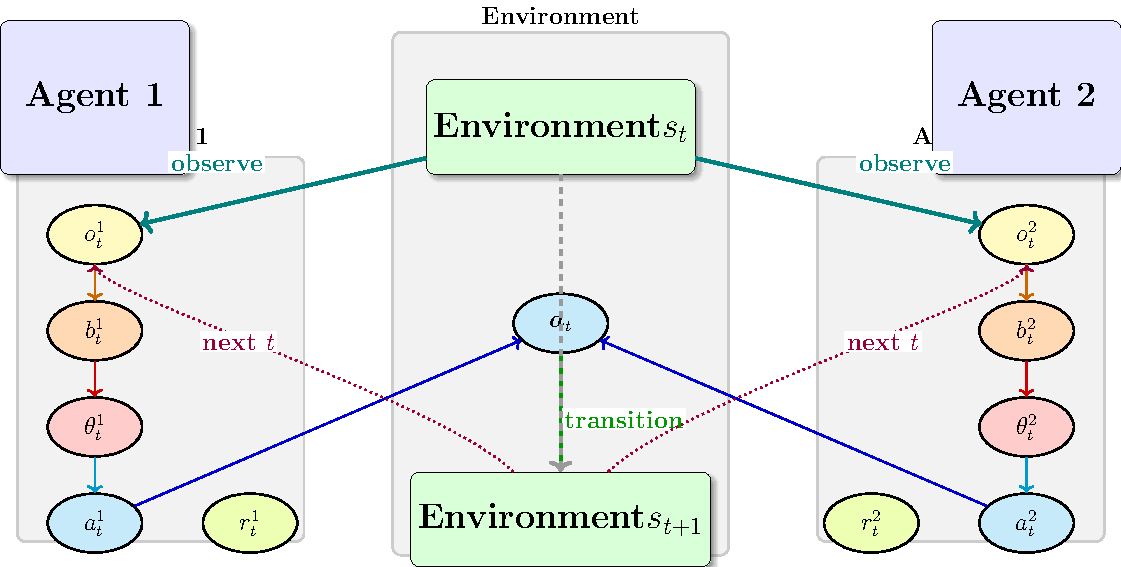
\includegraphics[width=0.9\linewidth]{figures/poamg-structure.pdf}
    \caption{Structure of a POAMGshowing the relationships between environment state, observations, beliefs, and policy parameters in a two-agent setting.}
    \label{fig:poamg-structure}
\end{figure}
\fi

In partially observable active Markov games, agents form beliefs to infer the underlying state of the environment. Unlike standard partially observable settings, these states evolve through the dynamically changing policies of the agents in addition to the environmental dynamics. The process unfolds as follows: at time step $t$, each agent $i$ selects an action at state $s_t \in S$ by sampling from its belief-conditioned policy $a^i_t \sim \pi^i(\cdot|b^i_t; \theta^i_t)$. When all agents act collectively through joint action $\boldsymbol{a_t}$, the environment transitions from $s_t$ to $s_{t+1}$ with probability $T(s_{t+1}|s_t, \boldsymbol{a}_t)$. Subsequently, each agent $i$ receives a reward $r^i_t = R^i(s_t, \boldsymbol{a}_t)$ and adjusts its policy parameters via the update function $U^i(\theta^i_{t+1}|\theta^i_t, \tau^i_t)$, where $\tau^i_t = \{o_t^i, \boldsymbol{a_t}, r^i_t, o_{t+1}^i\}$ is the trajectory for agent $i$ at time $t$ consisting of the current observation $o_t^i$, joint action $\boldsymbol{a_t}$, reward received $r^i_t$, and the next observation $o_{t+1}^i$. This adaptive cycle continues until non-stationary policies reach convergence. A key insight is that the joint policy update function $\boldsymbol{U}$ depends on $a^i_t$, which directly impacts state transitions and rewards, thereby enabling agent $i$ to strategically shape future collective policies through its individual decisions. This explicit modeling of strategic influence constitutes the primary advantage of active Markov games over their stationary counterparts.

\section{Convergence}
A central question in our analysis is whether the joint process of states, beliefs and policy parameters converges to a well-defined stationary distribution, and under what conditions. Following \citet{kim2022influencing}, we establish this connection using the properties of regularly perturbed Markov processes. First, we define the joint process, which operates on the joint space of states, beliefs and policy parameters.

\begin{definition}[Joint Process]
    In a Partially Observable Active Markov Game, the joint process $(s_t, \boldsymbol{b}_t, \boldsymbol{\theta}_t)$ consists of the state $s_t \in S$, the joint belief state $\boldsymbol{b}_t = (b^1_t, \ldots, b^n_t) \in \boldsymbol{B}$ and joint policy parameters $\boldsymbol{\theta}_t = (\theta^1_t, \ldots, \theta^n_t) \in \boldsymbol{\Theta}$ of all agents at time $t$.
\end{definition}
We then make the following assumptions on the subprocesses to ensure the ergodicity of the perturbed joint process.
\begin{assumption}[Communicating State Transition]\label{assumption:1}
    The state transition $T$ is communicating, meaning that for any two states $s, s' \in S$, there exists a sequence of joint actions $\boldsymbol{a}_1, \boldsymbol{a}_2, \ldots, \boldsymbol{a}_k$ and a sequence of states $s_1, s_2, \ldots, s_{k-1}$ such that:
    \begin{align}
        T(s_1|s, \boldsymbol{a}_1) > 0, \quad T(s_2|s_1, \boldsymbol{a}_2) > 0, \quad \ldots, \quad T(s'|s_{k-1}, \boldsymbol{a}_k) > 0
    \end{align}
\end{assumption}

\begin{assumption}[Communicating Belief-State Process]\label{assumption:2}
    The belief-state process is communicating, meaning that for any two belief states $b^i, b'^i \in B^i$, there exists a sequence of joint actions $\boldsymbol{a}_1, \boldsymbol{a}_2, \ldots, \boldsymbol{a}_m$ and a sequence of observations $o^i_1, o^i_2, \ldots, o^i_m$ such that:
    \begin{align}
        \mathbb{P}(b^i_{t+m} = b'^i | b^i_t = b^i, \boldsymbol{a}_t = \boldsymbol{a}_1, o^i_{t+1} = o^i_1, \ldots, \boldsymbol{a}_{t+m-1} = \boldsymbol{a}_m, o^i_{t+m} = o^i_m) > 0
    \end{align}
\end{assumption}
Assuming the communicating property of the subprocesses, we can establish convergence of the perturbed joint process to the unique stochastically stable distribution of the unperturbed one, as the perturbation vanishes in the limit.
\begin{theorem}[Stochastically Stable Distribution]
    Under Assumptions \ref{assumption:1} and \ref{assumption:2}, as $\epsilon \to 0$, the perturbed joint processes defined by $\epsilon$-perturbed policy update functions converge to the unique stochastically stable distribution $\mu^*$ of the unperturbed joint process $(s_t, \boldsymbol{b}_t, \boldsymbol{\theta}_t)$.
\end{theorem}

\begin{proof}
    See Appendix \ref{appendix:stochasticallystable} for a detailed proof.
\end{proof}
This convergence result has profound implications for our framework. By establishing the existence of a unique stochastically stable distribution, we provide a solid theoretical foundation for defining optimization objectives and analyzing equilibrium behavior in partially observable active Markov games. The stochastically stable distribution represents the limiting behavior of the system, independent of initial conditions, allowing us to characterize the long-run outcomes of social learning processes. This property is crucial for developing algorithms that optimize for long-term performance rather than myopic rewards, aligning with our goal of modeling sophisticated social learning dynamics. This property is crucial for developing algorithms that optimize for long-term performance rather than myopic rewards, aligning with our goal of modeling sophisticated social learning dynamics.

\section{Incentives}
We now formalize the optimization objectives for agents in our Partially Observable Active Markov Game framework. In contrast to traditional reinforcement learning settings that typically employ discounted rewards, we first focus on the average reward criterion as our fundamental optimization objective.
The average reward formulation provides several compelling advantages for modeling social learning dynamics. As \citet{sutton2018reinforcement} emphasize, this approach is particularly well-suited for continuing tasks without natural episode boundaries—a characteristic that aligns perfectly with the ongoing nature of social learning interactions. While economic theory has predominantly employed discounted reward objectives due to their mathematical tractability and natural correspondence to time preference in utility maximization \citep{koopmans1960stationary, stokey1989recursive}, the average reward paradigm better captures the strategic considerations in our framework.
The key advantage of the average reward approach in our context is its emphasis on the limiting behavior of the multi-agent system. When agents engage in repeated strategic interactions over indefinite horizons, their primary concern becomes the long-run system behavior rather than transient dynamics. Moreover, unlike discounted objectives that can induce myopic behavior depending on the discount factor, the average reward formulation naturally encourages agents to consider the permanent effects of their actions on other agents' learning processes—a crucial aspect for accurately modeling the strategic dimensions of social learning.

\begin{definition}[Average Reward Objective under Partial Observability]
    Each agent $i \in I$ in a Partially Observable Active Markov Game aims to find policy parameters $\theta^i$ and update function $U^i$ that maximize its expected average reward $\rho^i \in \mathbb{R}$ based on the joint beliefs $\boldsymbol{b}$:
    \begin{align}
        \begin{split}
            \max_{\theta^i, U^i} \rho^i(\boldsymbol{b}, \boldsymbol{\theta}, \boldsymbol{U}) : & = \max_{\theta^i, U^i} \lim_{T \to \infty} \mathbb{E}\left[\frac{1}{T}\sum_{t=0}^T R^i(s_t, \boldsymbol{a}_t) \Bigg|
                \begin{array}{c}
                    \boldsymbol{b}_0= \boldsymbol{b}, \boldsymbol{\theta}_0= \boldsymbol{\theta}, \\
                    \boldsymbol{a}_t \sim \boldsymbol{\pi}(\cdot|\boldsymbol{b_t}; \boldsymbol{\theta_t}),
                    s_{t+1} \sim T(\cdot|s_t, \boldsymbol{a}_t),        \\
                    \boldsymbol{o}_{t+1} \sim \boldsymbol{O}(\cdot|s_{t+1}),
                    \boldsymbol{\theta}_{t+1} \sim \boldsymbol{U}(\cdot|\boldsymbol{\theta_t}, \boldsymbol{\tau_t})
                \end{array}
            \right]                                                                                                                                                                                                                                                                                                                          \\
                                                                                               & = \max_{\theta^i, U^i} \sum_{s, \boldsymbol{b}, \boldsymbol{\theta}} b^i(s) \mu^*(s, \boldsymbol{b}, \boldsymbol{\theta}) \sum_{\boldsymbol{a}} \boldsymbol{\pi}(\boldsymbol{a}|\boldsymbol{b}; \boldsymbol{\theta}) R^i(s, \boldsymbol{a})
        \end{split}
    \end{align}


\end{definition}

This formulation emphasizes that agents aim to maximize their rewards in the limiting behavior of the Markov process, focusing on long-term performance rather than immediate gains. The second equality expresses the objective in terms of the stochastically stable distribution $\mu^*$, weighted by agent's belief, connecting our optimization problem to the theoretical results established earlier. It is worth noting that this definition assumes beliefs, policy parameters, and policy update functions are all publicly observable. Since this assumption rarely holds in practical scenarios, we will implement \textit{variational inference} in our algorithm to enable agents to infer these measures from their partial observations. Next, we derive the policy gradients, which we will be the foundation of our algorithm, allowing the agents to maximize their objectives.

\section{Belief-Based Policy Gradients}
Policy gradient methods are a class of reinforcement learning techniques that directly optimize policy parameters by following the gradient of expected return~\cite{sutton1999policy}. Unlike value-based methods, policy gradients explicitly parametrize the policy and update parameters in the direction that improves performance. These methods excel in continuous action spaces and can learn stochastic policies~\cite{williams1992simple}. In partially observable settings, policy gradients require adaptation to handle belief states rather than true states~\cite{kaelbling1998planning}. Modern approaches like Proximal Policy Optimization~\cite{schulman2017proximal} have further improved stability and sample efficiency of these methods through constrained policy updates.

Our framework extends these concepts to multi-agent settings with non-stationary policies by incorporating the Active Markov Game formulation of \citet{kim2022influencing}. The key innovation in our approach is conditioning value functions not just on belief states, but on the joint space of states, belief states, and policy parameters of all agents. This allows us to explicitly model how an agent's actions influence both the environmental dynamics and the learning processes of other agents.

While our theoretical framework proposes maximizing over both policy parameters $\theta^i$ and update functions $U^i$, this joint optimization presents significant computational challenges. As noted in \citet{kim2022influencing} optimizing over policy update functions essentially constitutes a long-horizon meta-learning problem, which remains computationally intractable for many realistic multi-agent settings. Following their practical approach, we simplify the optimization problem by focusing exclusively on learning optimal fixed-point policies that influence joint policy behavior while using standard update rules:

\begin{align}
    \max_{\theta^i} \rho^i_{\theta^i}(\boldsymbol{b}, \boldsymbol{\theta}) & := \max_{\theta^i} \lim_{T \to \infty} \mathbb{E}\left[ \frac{1}{T}\sum_{t=0}^T R^i(s_t, \boldsymbol{a}_t) \bigg|
        \begin{array}{c}
            \boldsymbol{b}_0= \boldsymbol{b}, \boldsymbol{\theta}_0= \boldsymbol{\theta}, \\
            \boldsymbol{a}_t \sim \boldsymbol{\pi}(\cdot|\boldsymbol{b}_t; \boldsymbol{\theta}_t),
            s_{t+1} \sim T(\cdot|s_t, \boldsymbol{a}_t),                                  \\
            \boldsymbol{o}_{t+1} \sim \boldsymbol{O}(\cdot|s_{t+1}),
            \boldsymbol{\theta}_{t+1} \sim \boldsymbol{U}(\cdot|\boldsymbol{\theta}_t, \boldsymbol{\tau}_t)
        \end{array}
        \right]
\end{align}

This formulation still preserves the essence of our framework—capturing how agent $i$'s actions influence other agents' learning trajectories—while making the optimization problem tractable. Under the stochastically stable distribution discussed earlier, this simplified objective becomes independent of initial conditions, further supporting the practical viability of our approach. Under the average reward formulation, we define the differential value function for agent $i$ as:

\begin{align}
    v^i_{\theta^i}(s, \boldsymbol{b}, \boldsymbol{\theta}) = \lim_{T \to \infty} \mathbb{E}\left[ \sum_{t=0}^T \left(R^i(s_t, \boldsymbol{a}_t) - \rho^i_{\theta^i}\right) \Bigg|
    \begin{array}{c}
        s_0=s, \boldsymbol{b}_0= \boldsymbol{b}, \boldsymbol{\theta}_0= \boldsymbol{\theta}, \\
        \boldsymbol{a}_t \sim \boldsymbol{\pi}(\cdot|\boldsymbol{b}_t; \boldsymbol{\theta}_t),
        s_{t+1} \sim T(\cdot|s_t, \boldsymbol{a}_t),                                         \\
        \boldsymbol{o}_{t+1} \sim \boldsymbol{O}(\cdot|s_{t+1}),
        \boldsymbol{\theta}_{t+1} \sim \boldsymbol{U}(\cdot|\boldsymbol{\theta}_t, \boldsymbol{\tau}_t)
    \end{array}
    \right]
\end{align}

This function represents the expected total difference between future rewards and the average reward $\rho^i_{\theta^i}$ when starting from state $s$, belief states $\boldsymbol{b}$, and policy parameters $\boldsymbol{\theta}$. It serves as a crucial component in deriving the policy gradient theorem for our framework.


\begin{theorem}[Partially Observable Active Average Reward Policy Gradient Theorem]
    \label{thm:avg_gradient}
    The gradient of the active average reward objective with respect to agent $i$'s policy parameters $\theta^i$ in a partially observable setting is:
    \begin{align}
        \nabla_{\theta^i} J^i_\pi(\theta^i) = \sum_{s, \boldsymbol{b}, \boldsymbol{\theta}} \mu_{\theta^i}(s, \boldsymbol{b}, \boldsymbol{\theta}) \sum_{a^i} \nabla_{\theta^i} \pi^i(a^i|b^i; \theta^i) \sum_{a^{\neg i}} \pi^{\neg i}(a^{\neg i}|b^{\neg i}; \theta^{\neg i}) q^i_{\theta^i}(s, \boldsymbol{b}, \boldsymbol{\theta}, \boldsymbol{a})
        \label{eq:avg_gradient}
    \end{align}

    where the action-value function $q^i_{\theta^i}$ is defined as:
    \begin{align}
        q^i_{\theta^i}(s, \boldsymbol{b}, \boldsymbol{\theta}, \boldsymbol{a}) = \sum_{s'} T(s'|s, \boldsymbol{a}) \sum_{\boldsymbol{o}'} \boldsymbol{O}(\boldsymbol{o}'|s') \sum_{\boldsymbol{\theta}'} \boldsymbol{U}(\boldsymbol{\theta}'|\boldsymbol{\theta}, \boldsymbol{\tau}) \left[ R^i(s, \boldsymbol{a}) - \rho^i_{\theta^i} + v^i_{\theta^i}(s', \text{update}(\boldsymbol{b}, \boldsymbol{a}, \boldsymbol{o}'), \boldsymbol{\theta}') \right]
        \label{eq:avg_action_value}
    \end{align}

    with $\text{update}(\boldsymbol{b}, \boldsymbol{a}, \boldsymbol{o}')$ representing the belief update function.

\end{theorem}

\begin{proof}
    See Appendix \ref{appendix:avg_gradient} for a detailed proof.
\end{proof}
This theorem extends the policy gradient result in \citet{kim2022influencing} to partially observable settings by integrating over the joint space of states, beliefs, and policy parameters according to their stochastically stable distribution $\mu_{\theta^i}(s, \boldsymbol{b}, \boldsymbol{\theta})$. The resulting gradient has a form similar to the standard policy gradient theorem, but with important modifications. First, our policies are conditioned on belief states rather than actual states. Second, the action-value function must account for belief updates and policy parameter evolution. Third, the expectation is taken over the stochastically stable distribution of the joint state space, while also considering the stochasticity of the observations.

Building on the theoretical foundations established for the average reward criterion, we now turn our attention to the discounted return formulation. This alternative objective function is particularly relevant in economic contexts where agents exhibit time preferences, valuing immediate rewards more highly than delayed ones. The following section develops the mathematical framework for optimizing agent behavior under discounted returns, providing a complementary perspective to our earlier analysis. By examining both criteria, we offer a comprehensive theoretical foundation that can accommodate different modeling assumptions about how agents value future consequences of their actions.

\section{Discounted Returns}

While the average reward criterion provides a principled approach for analyzing limiting behaviors in continuing tasks, the discounted return objective remains predominant in economic models of social learning \citep{keller2005strategic, bolton1999strategic, huang2024learning,brandl2024}. This formulation incorporates time preference through a discount factor $\gamma \in [0, 1)$, giving higher weight to near-term rewards and diminishing importance to those further in the future. The expected effective planning horizon under discounting is approximately $\frac{1}{1-\gamma}$ steps \citep{kearns2002near}, making it well-suited for scenarios where agents exhibit time preference or where finite planning horizons are appropriate \citep{frederick2002time, sutton2018reinforcement}. We begin by formalizing the discounted return objective in our POAMG framework:

\begin{definition}[Discounted Return Objective under Partial Observability]
    Each agent $i \in I$ in a Partially Observable Active Markov Game aims to find policy parameters $\theta^i$ that maximize its expected discounted return $J^i_{\pi, \gamma}(\theta^i) = v^i_{\theta^i}(s_0, \boldsymbol{b}_0, \boldsymbol{\theta}_0)$ starting from initial state $s_0$, joint beliefs $\boldsymbol{b}_0$, and joint policy parameters $\boldsymbol{\theta}_0$:
    \begin{align}
        \max_{\theta^i} v^i_{\theta^i}(s_0, \boldsymbol{b}_0, \boldsymbol{\theta}_0) & := \max_{\theta^i} \mathbb{E}\left[ \sum_{t=0}^{\infty} \gamma^t R^i(s_t, \boldsymbol{a}_t) \bigg|
            \begin{array}{c}
                s_0, \boldsymbol{b}_0, \boldsymbol{\theta}_0, \\
                \boldsymbol{a}_{0:\infty} \sim \boldsymbol{\pi}(\cdot|\boldsymbol{b}_{0:\infty}; \boldsymbol{\theta}_{0:\infty}),
                s_{t+1} \sim T(\cdot|s_t, \boldsymbol{a}_t),  \\
                \boldsymbol{o}_{t+1} \sim \boldsymbol{O}(\cdot|s_{t+1}),
                \boldsymbol{\theta}_{t+1} \sim \boldsymbol{U}(\cdot|\boldsymbol{\theta}_t, \boldsymbol{\tau}_t)
            \end{array}
            \right]
    \end{align}

\end{definition}

The discounted return objective differs fundamentally from the average reward criterion in its treatment of future consequences. As $\gamma$ approaches 1, it increasingly resembles the average reward formulation, but with a crucial distinction: even with $\gamma$ arbitrarily close to 1, the discounted formulation still assigns diminishing weight to distant future rewards. This property has significant implications for strategic behavior in multi-agent settings, particularly in social learning contexts.

\subsection{Discounted Visitation Measure}

To analyze the behavior of agents operating under discounted returns, we introduce the \textit{discounted visitation measure} (also called occupancy measure). This measure represents the normalized expected discounted time spent in each state-belief-policy configuration when following a joint policy \citep{sutton1999policy, Silver2014DeterministicPG}.

\begin{definition}[Discounted Visitation Measure]
    For a Markov process governed by a transition operator $\Psi$ and its adjoint $\Psi^*$, with an initial distribution $\mu_0$ over the joint state-belief-policy space, the discounted visitation measure $d^{\pi}_{\mu_0}$ is defined as:
    \begin{equation}
        d^{\pi}_{\mu_0} := (1-\gamma) \sum_{t=0}^{\infty} \gamma^t \mu_t
    \end{equation}

    where $\mu_t$ is the distribution at time $t$ when starting from $\mu_0$, and $\gamma \in [0, 1)$ is the discount factor.
\end{definition}

This distribution serves two critical purposes in our framework. First, it provides a well-defined distribution over which expectations can be taken, even in non-stationary environments where policies are constantly changing. Unlike the stochastically stable distribution used in the average reward setting, the discounted distribution automatically exists for any $\gamma < 1$ without requiring additional assumptions on the ergodicity of the underlying processes \citep{puterman1994markov}. Second, it directly links to the optimization objective, allowing us to express the expected discounted return as an expectation of immediate rewards under this distribution.

The discounted visitation measure satisfies important properties that facilitate policy optimization. Most notably, it can be expressed as the unique solution to a functional equation:

\begin{equation}
    d^{\pi}_{\mu_0} = (1-\gamma)\mu_0 + \gamma \Psi^* d^{\pi}_{\mu_0}
\end{equation}


where $\Psi^*$ is the adjoint of the transition operator $\Psi$ that describes how probability distributions evolve over one timestep. This relationship can be seen as a fixed-point equation, where $d^{\pi}_{\mu_0}$ is the unique fixed point of the contractive mapping $(1-\gamma)\mu_0 + \gamma \Psi^*(\cdot)$ in the space of finite measures. The existence and uniqueness of this measure is guaranteed for any $\gamma < 1$, providing a solid mathematical foundation for our policy gradient derivations.

\subsection{Policy Gradient Theorem for Discounted Returns}

With the discounted visitation measure established, we now derive the policy gradient theorem that forms the basis for optimization in this framework.
\begin{theorem}[Partially Observable Active Discounted Return Policy Gradient Theorem]
    \label{thm:discounted_gradient}
    The gradient of the discounted return objective $J^i_{\pi, \gamma}(\theta^i) = v^i_{\theta^i}(s_0, \boldsymbol{b}_0, \boldsymbol{\theta}_0)$ with respect to agent $i$'s policy parameters $\theta^i$ in a partially observable active Markov game setting can be expressed as:
    \begin{align}
        \nabla_{\theta^i} J^{i}_{\pi, \gamma}(\theta^i) & = \frac{1}{1-\gamma} \sum_{s, \boldsymbol{b}, \boldsymbol{\theta}} d^{\pi}_{\mu_0}(s, \boldsymbol{b}, \boldsymbol{\theta}) \sum_{a^i} \nabla_{\theta^i} \pi^i(a^i|b^i; \theta^i) \nonumber \\
                                                 & \quad \sum_{a^{-i}} \pi^{-i}(a^{-i}|\boldsymbol{b}^{-i}; \theta^{-i}) q^i_{\theta^i}(s, \boldsymbol{b}, \boldsymbol{\theta}, \boldsymbol{a})
        \label{eq:discounted_gradient}
    \end{align}

    where $d^{\pi}_{\mu_0}(s, \boldsymbol{b}, \boldsymbol{\theta})$ is the discounted visitation measure starting from initial distribution $\mu_0$, and $q^i_{\theta^i}(s, \boldsymbol{b}, \boldsymbol{\theta}, \boldsymbol{a})$ is the action-value function defined as:
    \begin{align}
        q^i_{\theta^i}(s, \boldsymbol{b}, \boldsymbol{\theta}, \boldsymbol{a}) & = R^i(s, \boldsymbol{a}) + \gamma \sum_{s'} T(s'|s, \boldsymbol{a}) \sum_{\boldsymbol{o}'} \boldsymbol{O}(\boldsymbol{o}'|s') \nonumber                                                                                \\
                                                                               & \quad \sum_{\boldsymbol{\theta}'} \boldsymbol{U}(\boldsymbol{\theta}'|\boldsymbol{\theta}, \boldsymbol{\tau}) v^i_{\theta^i}(s', \text{update}(\boldsymbol{b}, \boldsymbol{a}, \boldsymbol{o}'), \boldsymbol{\theta}')
    \label{eq:discounted_action_value}
                                                                            \end{align}

\end{theorem}

\begin{proof}
    See Appendix \ref{appendix:discounted_proofs} for a detailed proof.
\end{proof}

This theorem connects the policy gradient to expectations with respect to the discounted visitation measure, providing a principled approach to policy optimization in partially observable multi-agent settings. The scaling factor $\frac{1}{1-\gamma}$ accounts for the effective horizon of the discounted objective, with its magnitude increasing as $\gamma$ approaches 1.

In implementation, the choice between these objectives should be guided by the specific characteristics of the social learning scenario being modeled. The discounted formulation may be appropriate for settings with finite horizons, impatient agents, or where near-term performance is particularly valued. However, for scenarios focused on long-run learning dynamics and asymptotic behavior, the average reward criterion provides a more principled approach by equally valuing rewards across all future time periods.

In practice, computing these gradients exactly is typically infeasible. Instead, sample-based approximations and function approximation techniques using neural networks are employed to estimate the gradient from experience. Nevertheless, in theory, when agents learn to adapt their policies according to these gradients, they eventually converge to an equilibrium concept related to traditional equilibria, which we will introduce in the following section.

\section{Equilibrium}
Policy gradient optimization naturally leads agents toward stable configurations where no individual agent can unilaterally improve its reward by changing its policy. Given the formalization of our optimization objectives and the policy gradient theorems established above, we now characterize equilibrium concepts in Partially Observable Active Markov Games. By following the gradient directions specified in Theorems \ref{thm:avg_gradient} and \ref{thm:discounted_gradient}, agents can iteratively improve their policies to maximize their respective objectives. This optimization process naturally leads to the concept of Partially Observable Active Equilibrium, which extends the Active Equilibrium from standard Active Markov Games \cite{kim2022influencing} to account for partial observability while representing the fixed point of the policy gradient optimization process.

\begin{definition}[Partially Observable Active Equilibrium]
    A Partially Observable Active Equilibrium is a joint policy parameter $\boldsymbol{\theta}^* = \{\theta^{i*}, \theta^{-i*}\}$ with associated joint update function $\boldsymbol{U}^* = \{U^{i*}, U^{-i*}\}$ such that for all $i \in I$:
    \begin{align}
        J^i_{\pi}(\boldsymbol{b}, \theta^{i*}, \theta^{-i*}, U^{i*}, U^{-i*}) &\geq J^i_{\pi}(\boldsymbol{b}, \theta^i, \theta^{-i*}, U^i, U^{-i*}) \quad \text{(average reward case)} \\
        J^i_{\pi, \gamma}(\boldsymbol{b}, \theta^{i*}, \theta^{-i*}, U^{i*}, U^{-i*}) &\geq J^{i}_{\pi, \gamma}(\boldsymbol{b}, \theta^i, \theta^{-i*}, U^i, U^{-i*}) \quad \text{(discounted reward case)} 
    \end{align}
    
    for all $\boldsymbol{b} \in \boldsymbol{B}$, $\theta^i \in \Theta^i$, $U^i \in \mathcal{U}^i$, where $\mathcal{U}^i$ is the space of possible update functions for agent $i$.
\end{definition}

This equilibrium concept captures the idea that rational agents should optimize not just their immediate policies but also their adaptation strategies, taking into account the learning dynamics of the system while operating under partial observability. At equilibrium, no agent can improve its long-term reward (either discounted or average, depending on the formulation) by unilaterally changing either its policy or its update function, overlapping with the definition of the Bayesian Nash equilibrium in non-cooperative games.

Computing partially observable active equilibria exactly is typically intractable due to the complexity of belief spaces and the sophistication of policy update functions. Nevertheless, this equilibrium concept provides a theoretical benchmark against which practical algorithms can be evaluated. In the next section, we discuss the computational challenges inherent in direct implementation of our theoretical framework, before introducing our practical policy optimization method that approximates equilibrium strategies through policy gradient algorithms.

\section{Challenges with Exact Computation}

Theorems \ref{thm:avg_gradient} and \ref{thm:discounted_gradient} provide mathematically principled approaches for optimizing policies in both average and discounted return settings, but implementing them exactly is computationally infeasible for most real-world applications. In partially observable environments, agents must maintain belief states, whose evolution can be governed by the Bayes' rule as:

\begin{align}
    b^i_{t+1}(s') = \frac{O^i(o^i_{t+1}|s') \int_{s \in S} T(s'|s, \boldsymbol{a}_t) b^i_t(s) ds}{\int_{s'' \in S} O^i(o^i_{t+1}|s'') \int_{s \in S} T(s''|s, \boldsymbol{a}_t) b^i_t(s) ds ds''}
\end{align}

For environments with large or continuous state spaces, representing and updating these distributions becomes prohibitively expensive. Moreover, exact updates require perfect knowledge of observation functions $O^i$ and transition dynamics $T$, which may not be readily available to the agents. The complexity compounds in multi-agent settings where agents must reason about others' belief states and policies using Bayesian inference:

\begin{align}
    \mathbb{P}(\boldsymbol{b}^{-i}_t, \boldsymbol{\theta}^{-i}_t | \tau^i_{0:t}) \propto \mathbb{P}(\tau^i_{0:t} | \boldsymbol{b}^{-i}_t, \boldsymbol{\theta}^{-i}_t) \mathbb{P}(\boldsymbol{b}^{-i}_t, \boldsymbol{\theta}^{-i}_t | \tau^i_{0:t-1})
\end{align}

This creates nested inference problems—agents maintaining beliefs about others' beliefs—that grow exponentially with the number of agents and the complexity of their policies. 

Computing action-value functions adds another layer of intractability, with different formulations for average returns and discounted returns. The triple expectations—over next states, observations, and policy parameters— in equations \eqref{eq:avg_action_value} and \eqref{eq:discounted_action_value} require summing over an exponentially large joint space, where the policy parameter space $\Theta^i$ would ideally be modified to be continuous. Furthermore, the policy update functions $\boldsymbol{U}$ of other agents are typically unknown, and the recursive nature of the value function creates computational dependencies that quickly become unmanageable. 

The policy gradient calculations presented in Equations \eqref{eq:avg_gradient} and \eqref{eq:discounted_gradient} present similarly insurmountable difficulties. Computing the stochastically stable distribution $\mu_{\theta^i}(s, \boldsymbol{b}, \boldsymbol{\theta})$ for average returns or the discounted visitation measure $d^{\pi}_{\mu_0}(s, \boldsymbol{b}, \boldsymbol{\theta})$ for discounted returns requires implementing additional algorithms \citep{wicks2012algorithmcomputingstochasticallystable}, while expectations over joint actions create additional combinatorial explosion. These computational barriers—state space explosion, nested belief inference, triple expectations, and distribution computation—collectively render exact computation infeasible except for trivial environments. The curse of dimensionality is especially severe due to the combined complexity of partial observability, multi-agent interactions, and evolving policies. 

To address these computational challenges and make our theoretical framework practically applicable, we develop POLARIS, a neural network-based algorithm that approximates the key components of our framework while maintaining its essential properties.

\section{Algorithm: POLARIS}

In this section, we present POLARIS (Partially Observable Learning with Active Reinforcement In Social environments), our practical implementation of the theoretical framework. POLARIS extends and improves upon the FURTHER algorithm \cite{kim2022influencing} with specialized components for belief modeling, information propagation through networks, and advantage-weighted training. The algorithm uses neural network approximations to overcome the computational challenges outlined in the previous section while preserving the key insights of our theoretical framework. It consists of three integrated modules: a belief processing module, an inference learning module, and a reinforcement learning module, which operate in concert to enable sophisticated social learning in partially observable environments. The architecture integrates several neural network components working in tandem: a Transformer-based belief processor~\cite{vaswani2017attention} provides sophisticated temporal pattern recognition through its self-attention mechanisms; a Temporal Graph Neural Network (GNN) with multi-head attention for network-aware representations; and Soft Actor-Critic (SAC) with dual Q-networks supporting discrete action spaces and both average and discounted reward formulations. We provide the detailed network architectures in Appendix \ref{appendix:neural_architectures}.

\subsection{Belief Processing Module}

The belief processing module employs a Transformer architecture to encode the agent's belief state based on partial observations and joint actions:

\begin{align}
    b^i_t = f_{\text{Transformer}}(b^i_{t-1}, o^i_t, \boldsymbol{a}_{t-1}; \psi^i_{\text{Transformer}})
\end{align}

Unlike traditional recurrent approaches, the Transformer architecture introduces crucial advantages for social learning scenarios. The self-attention mechanism allows the model to weigh the importance of different parts of the observation history dynamically, enabling it to focus on the most informative signals while downplaying noise or irrelevant information. By processing inputs in parallel rather than sequentially, the Transformer enables more efficient training compared to conventional Recurrent Neural Networks, particularly important when dealing with multiple agents and long interaction histories. Perhaps most importantly for social learning, the Transformer architecture captures relationships between temporally distant observations more effectively, allowing agents to recognize patterns that may emerge over extended periods of social interaction. The Transformer-based belief processor also outputs an explicit belief distribution over possible states:

\begin{align}
    \mathbb{P}(s|b^i_t) = \text{Softmax}(f_{\text{belief\_head}}(b^i_t)) 
\end{align}

This explicit representation provides transparency into decision-making processes and facilitates debugging and analysis of social learning dynamics.

The belief processor is trained using different objectives depending on the signal type. For discrete signals, it uses a standard cross-entropy loss to track the underlying state distribution:
\begin{align}
    J^i_{\text{transformer,discrete}}(\psi^i_{\text{Transformer}}) = \mathbb{E}_{D^i}\left[-\log \mathbb{P}(s_t|b^i_t; \psi^i_{\text{Transformer}})\right]
\end{align}

For continuous signals (such as Lévy processes), POLARIS employs a specialized transformer loss function that computes the expected signal distribution based on the current belief state and environment parameters:
\begin{align}
    J^i_{\text{transformer,continuous}}(\psi^i_{\text{Transformer}}) = \mathbb{E}_{D^i}\left[\|o^i_t - \hat{o}^i_t(b^i_t, \text{env\_params}; \psi^i_{\text{Transformer}})\|^2\right]
\end{align}

where $D^i$ is agent $i$'s replay buffer containing stored transitions, $\hat{o}^i_t$ is the predicted continuous signal based on the belief state and environment parameters. This ensures that the belief processor maintains accurate state estimation capabilities for both discrete and continuous observation types throughout training.

\subsection{Inference Learning Module}

POLARIS implements a Temporal Graph Neural Network (GNN) with multi-head attention for network-aware social learning. This inference module represents the multi-agent system as a dynamic graph where nodes correspond to agents and edges represent observational relationships that are automatically inferred from the neighbor actions tensor. The module supports both discrete and continuous signal processing through separate GNN pathways:

\begin{align}
    \mu_t, \log\sigma_t = \text{TemporalGNN}(o^i_t, \boldsymbol{a}_t, r^i_t, o^i_{t+1}; \phi^i_{\text{GNN}})
\end{align}

The network topology is dynamically constructed from observed neighbor actions, where non-zero entries indicate actual neighbors (edges exist) and zero entries indicate non-neighbors (no edges). This approach enables automatic adaptation to various social network structures without requiring explicit network specification.

Key architectural features include dual-pathway processing that employs separate Graph Attention Network (GAT) layers for discrete (one-hot encoded) and continuous signals, enabling flexible handling of different observation types. The system incorporates multi-head attention mechanisms that operate both spatially (based on network topology) and temporally, differentially weighing connections based on decision relevance. A temporal memory system maintains past node features and edge indices through a sliding window buffer for temporal attention computation. The architecture leverages Graph Attention Networks (GAT) with multiple GAT layers containing attention heads that learn to focus on the most relevant neighboring agents.

The inference module learns a mapping from observable trajectories to latent variables predictive of other agents' behaviors, optimized using the Evidence Lower Bound (ELBO) objective \citep{kim2022influencing}:

\begin{align}
    J^i_{\text{elbo}} = \mathbb{E}_{\mathbb{P}(\tau^i_{0:t}),\mathbb{P}(\boldsymbol{\hat{z}}^{-i}_{1:t}|\tau^i_{0:t-1};\phi^i_{\text{GNN}})}\left[ \sum_{t'=1}^t \log \mathbb{P}(\boldsymbol{a}^{-i}_{t'}|o^i_{t'}, \boldsymbol{\hat{z}}^{-i}_{t'}; \phi^i_{\text{GNN}}) \right. \\
    \left. - \alpha_{KL} D_{KL}(\mathbb{P}(\boldsymbol{\hat{z}}^{-i}_{t'}|\tau^i_{t'-1}; \phi^i_{\text{GNN}})||\mathbb{P}(\boldsymbol{\hat{z}}^{-i}_{t'-1}))\right]
\end{align}

The ELBO objective balances reconstruction accuracy (predicting other agents' actions) with temporal consistency through a temporal KL divergence term that encourages smooth evolution of latent representations over time:

\begin{align}
    D_{KL}^{\text{temporal}} = \frac{1}{2} \mathbb{E}_t \left[ \log \frac{|\boldsymbol{\Sigma}_{t-1}|}{|\boldsymbol{\Sigma}_t|} - d + \text{tr}(\boldsymbol{\Sigma}_{t-1}^{-1}\boldsymbol{\Sigma}_t) + (\boldsymbol{\mu}_{t-1} - \boldsymbol{\mu}_t)^T \boldsymbol{\Sigma}_{t-1}^{-1} (\boldsymbol{\mu}_{t-1} - \boldsymbol{\mu}_t) \right]
\end{align}

where $\boldsymbol{\mu}_t$ and $\boldsymbol{\Sigma}_t$ are the mean and covariance of the latent distribution at time $t$. This temporal smoothing prevents abrupt changes in opponent models that could destabilize learning dynamics.

\subsection{Reinforcement Learning Module}

The reinforcement learning module uses the Soft Actor-Critic (SAC) framework with dual Q-networks and entropy regularization. The implementation supports discrete action spaces:

\begin{align}
    \pi^i(a^i|b^i, \boldsymbol{\hat{z}}^{-i}; \theta^i) &= \text{Categorical}(a^i|\text{MLP}_{\text{policy}}(b^i, \boldsymbol{\hat{z}}^{-i}; \theta^i)) \\
    q^i_{\theta^i}(b^i, \boldsymbol{\hat{z}}^{-i}, \boldsymbol{a}; \psi^i_{\beta}) &= \text{MLP}_{\text{value}}(b^i, \boldsymbol{\hat{z}}^{-i}, \boldsymbol{a}; \psi^i_{\beta})
\end{align}

where MLP stands for \emph{Multi Layer Perceptron}. The SAC framework's entropy regularization promotes exploration and prevents premature convergence to suboptimal equilibria, crucial in partially observable settings where perfect inference is impossible.

The RL module optimizes three objectives:

\subparagraph{Value Function Objective} POLARIS supports both discounted and average reward formulations. For discounted returns:
\begin{align}
    J^i_q(\psi^i_{\beta}) &= \mathbb{E}_{D^i}\left[(y - q^i_{\theta^i}(b^i, \boldsymbol{\hat{z}}^{-i}, \boldsymbol{a}; \psi^i_{\beta}))^2\right] \\
    y &= r^i + \gamma \cdot \min_{\beta=1,2} q^i_{\theta^i}(b^i_{t+1}, \boldsymbol{\hat{z}}^{-i}_{t+1}, a'^i; \bar{\psi}^i_{\beta})
\end{align}

For average reward (with automatically estimated average reward rate $\rho^i$):
\begin{align}
    J^i_q(\psi^i_{\beta}, \rho^i) &= \mathbb{E}_{D^i}\left[(y - q^i_{\theta^i}(b^i, \boldsymbol{\hat{z}}^{-i}, \boldsymbol{a}; \psi^i_{\beta}))^2\right] \\
    y &= r^i - \rho^i + \min_{\beta=1,2} q^i_{\theta^i}(b^i_{t+1}, \boldsymbol{\hat{z}}^{-i}_{t+1}, a'^i; \bar{\psi}^i_{\beta})
\end{align}

\subparagraph{Policy Objective} Maximizes expected value plus entropy:
\begin{align}
    J^i_{\pi}(\theta^i) &= \mathbb{E}_{D^i}\left[\mathbb{E}_{a^i \sim \pi^i}\left[\min_{\beta=1,2} q^i_{\theta^i}(b^i, \boldsymbol{\hat{z}}^{-i}, a^i, \boldsymbol{a}^{-i}; \psi^i_{\beta}) + \alpha_e H(\pi^i(\cdot|b^i, \boldsymbol{\hat{z}}^{-i}; \theta^i))\right]\right]
\end{align}

\subsection{Training Process}

The training process interleaves updates across all modules within each iteration. Algorithm 1 outlines the complete POLARIS training procedure.

\begin{algorithm}[!htbp]
\caption{POLARIS Training Algorithm for Single Agent}
\begin{algorithmic}[1]
\State Initialize belief processor, inference GNN, policy and Q-networks with parameters $\psi^i_{\text{Transformer}}$, $\phi^i_{\text{GNN}}$, $\theta^i$, $\psi^i_{\beta}$
\State Initialize replay buffer $D^i$, initial belief $b^i_0$, and latent state $\boldsymbol{\hat{z}}^{-i}_0$
\State Initialize target networks
\For{each step $t$}
    \State Observe signal $o^i_t$ and neighbor actions $\boldsymbol{a}^{-i}_{t-1}$
    \State Update belief: $b^i_t, \mathbb{P}(s|b^i_t) = f_{\text{Transformer}}(b^i_{t-1}, o^i_t, \boldsymbol{a}_{t-1}; \psi^i_{\text{Transformer}})$
    \State Construct graph and infer latent: $\boldsymbol{\hat{z}}^{-i}_t = f_{\text{GNN}}(o^i_t, \boldsymbol{a}^{-i}_t, r^i_{t-1}, o^i_{t-1}; \phi^i_{\text{GNN}})$
    \State Select action: $a^i_t \sim \text{Categorical}(\pi^i(\cdot|b^i_t, \boldsymbol{\hat{z}}^{-i}_t; \theta^i))$
    \State Execute action, observe reward $r^i_t$ and next signal $o^i_{t+1}$
    \State Store $(o^i_t, b^i_t, \boldsymbol{\hat{z}}^{-i}_t, a^i_t, r^i_t, o^i_{t+1}, \boldsymbol{a}^{-i}_t)$ in replay buffer $D^i$
    \If{update step}
        \State Sample sequential batch $B$ from replay buffer $D^i$
        \State Update inference GNN: $\phi^i_{\text{GNN}} \leftarrow \phi^i_{\text{GNN}} - \alpha_{\phi} \nabla_{\phi^i_{\text{GNN}}} J^i_{\text{elbo}}(B)$
        \State Update dual Q-networks: $\psi^i_{\beta} \leftarrow \psi^i_{\beta} - \alpha_{\psi} \nabla_{\psi^i_{\beta}} J^i_{q}(B)$
        \State Update policy: $\theta^i \leftarrow \theta^i - \alpha_{\theta} \nabla_{\theta^i} J^i_{\pi}(B)$
        \State Update belief processor: $\psi^i_{\text{Transformer}} \leftarrow \psi^i_{\text{Transformer}} - \alpha_{\psi} \nabla_{\psi^i_{\text{Transformer}}} J^i_{\text{transformer}}(B)$
        \State Update target networks: $\bar{\psi}^i_{\beta} \leftarrow \tau \psi^i_{\beta} + (1-\tau) \bar{\psi}^i_{\beta}$
    \EndIf
\EndFor
\end{algorithmic}
\end{algorithm}

Key implementation details include sequential batch sampling, where the replay buffer maintains sequential trajectories and samples sequences rather than individual transitions, preserving temporal dependencies crucial for transformer and GNN processing. The system employs dual Q-network updates with both Q-networks updated simultaneously using minimum value selection to prevent overestimation bias. All networks utilize gradient clipping with gradient norm clipping to maintain training stability. Target networks implement soft updates using exponential moving averages for stable learning.

In the next chapter, we demonstrate the practical application of our POAMG framework and the POLARIS algorithm to canonical social learning scenarios from economic theory. The versatility of our approach is particularly evident in its ability to handle both average and discounted reward formulations. This capability proves essential when implementing strategic experimentation and learning without experimentation models with discrete action spaces. Through these implementations, we validate theoretical predictions from economic models while uncovering new insights about strategic adaptation in partially observable multi-agent systems that would be difficult to obtain through purely analytical approaches. The experimental results not only demonstrate the effectiveness of our theoretical framework but also highlight how computational methods can complement and extend traditional economic analysis of social learning phenomena.


\chapter{Evaluation}
Building on the theoretical framework of Partially Observable Active Markov Games developed in the previous section, we now apply our POLARIS algorithm to concrete social learning scenarios: strategic experimentation and learning without experimentation. This implementation demonstrates how our approach bridges theoretical economic models with computational reinforcement learning methods, allowing us to validate theoretical predictions while uncovering new insights about strategic adaptation in partial observability settings.\footnote{Complete Python implementation is available at \url{https://github.com/ecdogaroglu/polaris}.}

\section{Methodological Framework and Challenges}

Theoretical frameworks —both in economics and in our POAMG framework— envision agents developing strategies that perform optimally across all possible states of the world. This \emph{ex ante} perspective requires agents to maintain flexibility and develop sophisticated mixed approaches that can respond appropriately regardless of which state is ultimately realized. Agents should learn conditional strategies of the form "if state = A, do X; if state = B, do Y," accounting for uncertainty about the true environmental state. 

The computational approach, however, reveals a fundamental departure from this theoretical ideal. Reinforcement learning agents instead converge to state-specific optimal allocations—an \emph{ex post} perspective where behavior is optimized for the particular state that has been realized. This distinction creates a critical incompatibility in the social learning environments we study, particularly due to their fixed-state structure.

To understand why this incompatibility emerges, consider the nature of optimal behavior in social learning environments with binary state spaces. In strategic experimentation, if the risky arm is good, rational agents should allocate all resources to it; conversely, if it performs poorly, optimal behavior requires complete avoidance. Similarly, in learning without experimentation, once the true state is A, the optimal action is unambiguously action A, while in state B, only action B is rational. These ex post strategies represent fundamentally incompatible policy objectives that cannot be reconciled through standard learning approaches.

The fixed-state structure of social learning models compounds this challenge. In each episode, agents can only observe and learn from one realized state, forcing them away from the ex ante strategies that theoretical frameworks prescribe. Instead of developing belief-contingent policies, agents learn "do X" during episodes with state A, then encounter conflicting objectives to "do Y" during subsequent episodes with state B. 

One natural approach to address this limitation would be to train agents across different environmental configurations, then evaluate their behavior under the full spectrum of possible conditions. However, this approach consistently fails due to a fundamental constraint of neural network learning. When network parameters are continuously updated across episodes, action-value functions adapt to the most recent state, leading to policies that are only optimal for the last state encountered. This phenomenon—known as \emph{catastrophic forgetting}—fundamentally constrains model evaluation for ex ante analysis.

\subsection{Catastrophic Forgetting in Fixed-State Social Learning}

Catastrophic forgetting represents a fundamental limitation in neural network learning where the acquisition of new knowledge systematically interferes with previously learned information \citep{vandeven2024continuallearningcatastrophicforgetting}. This phenomenon occurs when neural networks, optimized through gradient descent, overwrite previously learned weights and representations as they adapt to new tasks or environments. While various techniques have been developed to mitigate this issue in continual learning scenarios—including regularization methods, memory replay systems, and architectural approaches—these solutions typically assume some degree of compatibility or transferability between learning objectives \citep{kirkpatrick2017overcoming, zenke2017continuallearningsynapticintelligence, rebuffi2017icarl, rusu2016progressive}.


In our social learning environments, this compatibility assumption fails completely. When the optimal policy in state A requires action X while the optimal policy in state B demands the opposite action Y, no meaningful knowledge transfer is possible between episodes with different state realizations. The literature on negative transfer confirms that attempting to force knowledge sharing between fundamentally incompatible tasks degrades performance rather than enhancing it \citep{ahn2024catastrophic, wu2021online}. Traditional continual learning mechanisms that aim to "consolidate" or "protect" previous learning become counterproductive when such protection would directly undermine the acquisition of conflicting but equally necessary knowledge.

These fundamental constraints require us to reset agent parameters at the beginning of each episode rather than allowing continuous learning across state realizations. While this methodological necessity prevents direct measurement of the equilibrium strategies that economic theory and our POAMG framework predict, it does not invalidate our computational approach. Rather, it compels us to develop alternative analytical methodologies that can extract meaningful insights about multi-agent strategic behavior despite these inherent limitations of applying reinforcement learning to environments with conflicting learning objectives.

Our experimental methodology therefore focuses on within-episode learning dynamics and cross-episode pattern analysis. By examining how agents adapt their behavior within episodes and identifying systematic patterns across episodes, we can still characterize the essential features of multi-agent social learning, even when direct equilibrium convergence measurement is precluded by computational limitations.

\subsection{Two-Staged Analysis Methodology}
\label{sec:two-staged-analysis}

To address the catastrophic forgetting limitation while still extracting meaningful insights about multi-agent learning patterns, we adopt a consistent two-staged analysis approach across both experimental scenarios. This methodology enables robust characterization of learning dynamics despite the fundamental constraints of applying reinforcement learning to environments with fixed but episode-varying states.

\paragraph{Stage 1: Within-Episode Role Identification} For each episode $e$, we identify agents that exhibit extreme performance characteristics. In strategic experimentation, we track cumulative allocation patterns:
\begin{equation}
    i_{\text{high}}^e = \arg\max_i \sum_{t=1}^T a_{t,e}^i, \quad 
    i_{\text{low}}^e = \arg\min_i \sum_{t=1}^T a_{t,e}^i
\end{equation}

In learning without experimentation, we identify the fastest and slowest learning agents by fitting learning rates:
\begin{equation}
    i_{\text{fast}}^e = \arg\max_i r_e^i, \quad 
    i_{\text{slow}}^e = \arg\min_i r_e^i
\end{equation}
where $r_e^i$ is agent $i$'s learning rate in episode $e$.

\paragraph{Stage 2: Cross-Episode Pattern Aggregation} We then aggregate the performance of identified extreme agents across episodes to examine systematic patterns:
\begin{equation}
    \bar{P}_t^{\text{extreme}} = \frac{1}{n_{\text{episodes}}} \sum_{e=1}^{n_{\text{episodes}}} P_{t,e}^{i_{\text{extreme}}^e}
\end{equation}
where $P_{t,e}^i$ represents the relevant performance metric (cumulative allocation, learning accuracy, etc.) for agent $i$ at time $t$ in episode $e$.

This methodology reveals whether observed disparities represent structural features of multi-agent learning or merely artifacts of specific agent characteristics like network position, as different agents assume extreme roles across different episodes.

\section{Strategic Experimentation}

We reformulate the strategic experimentation model of \citet{keller2020undiscounted} as a Partially Observable Active Markov Game. This framework analyzes undiscounted continuous-time games where a number of symmetric players act non-cooperatively, trying to learn an unknown state of the world governing the risky arm's expected payoff. The state space $S = \{0,1,\ldots,m\}$ represents possible states of the world, with a deterministic transition function since the underlying state remains constant throughout the interaction. Each agent's action space in the theoretical model is $A^i = [0,1]$ representing the fraction of resources allocated to the risky arm at each decision point.

While the original model operates in continuous time with Lévy processes, our POAMG implementation discretizes time using the Euler-Maruyama scheme \citep{kloeden1992numerical, platen1999introduction} for both the background signal and the agents' payoff processes. However, to enable reinforcement learning with discrete action spaces, we implement a practical discretization where agents choose between two actions: "allocate to risky arm" (action 1) or "allocate to safe arm" (action 0). The probability of selecting action 1 serves as the continuous allocation parameter, allowing us to recover the continuous allocation behavior while maintaining compatibility with discrete policy networks.

The agents receive a public signal produced by the background process, which leads to the observation function:

\begin{equation}
    O^i(s, o) = \mathbb{P}(o_t | B_{t-1:t})
\end{equation}

where $o_t$ represents the observation at discrete time step $t$ and $B_{t-1:t}$ represents the signal increment in discrete time. To address the time-dependent nature of Lévy processes while maintaining compatibility with our POAMG framework, we formulate the reward function for each agent $i$ as:

\begin{equation}
    R^i(s, a^i) = (1-a^i)r_\textit{safe} + a^i \frac{X^i_{t-1:t}}{\Delta t}
\end{equation}
where $\Delta t$ is the discretization time step,
\begin{equation}
    X^i_{t-1:t} = \alpha_s \Delta t + \sigma (W^i_t - W^i_{t-1}) + \Delta Y^i_t,
\end{equation}
$(W^i_t - W^i_{t-1}) \sim \mathcal{N}(0, \Delta t)$, and $\Delta Y^i_t$ is the increment of the compound Poisson processes over the interval $[t-1, t]$.
This normalization converts accumulated rewards to instantaneous reward rates, preserving the incentive structure of the original model. A comprehensive mathematical treatment of this discretization approach, including convergence properties and the preservation of strategic incentives, is provided in Appendix \ref{appendix:levy_discretization}.

Each agent observes the increments in the public background signal, their own payoff process (dependent on their allocation $a^i$ to the risky arm and the true state $\omega$), and the allocations together with the rewards of all other agents. For continuous signals, POLARIS agents use a specialized transformer loss function that computes the expected signal distribution based on the current belief state and environment parameters, enabling principled belief updating in response to Lévy process observations.

\subsection{Experimental Setup}

We implement comprehensive experiments using specialized experimental frameworks for both detailed single-configuration analysis and comparative analysis across different group sizes. Our experimental protocol examines group sizes of $n \in \{1, 2, 4, 8\}$ agents; safe payoff of $r_{\text{safe}} = 0.5$; drift rates of $[0, 1]$ for bad and good states respectively; jump rates of $[0, 0.1]$ with jump sizes of $[1.0, 1.0]$; background informativeness of $k_0 = 0.001$; and time discretization step of $\Delta t = 1.0$.

Following our two-staged analysis methodology, the POLARIS implementation tracks: (1) Convergence of individual agent allocation strategies to state-dependent optimal actions within episodes; (2) Belief fluctuations over time to assess the impact of neighbor action observation on learning; (3) Cumulative allocation disparities between highest and lowest allocators as a function of group size; and (4) Episode-wise analysis of allocation patterns across different true states (good vs. bad).

For each configuration, we run experiments for comparative sweeps across group sizes, focusing on the emergence of allocation patterns and their relationship to theoretical predictions. Our analysis emphasizes within-episode learning dynamics rather than cross-episode equilibrium convergence due to the catastrophic forgetting constraint.

\subsection{Results and Analysis}

Our experimental results reveal sophisticated strategic learning dynamics while highlighting key challenges in measuring theoretical equilibrium convergence in reinforcement learning settings. We examine three primary aspects of the learning behavior that provide insights into multi-agent strategic experimentation.

\begin{figure}[!htbp]
    \centering
    \begin{minipage}[t]{0.48\textwidth}
        \centering
        \includegraphics[width=\textwidth]{../code/polaris/docs/allocation_accuracy_over_time.png}
        \subcaption{Allocation accuracy over time.}
        \label{fig:allocation_accuracy_over_time}
    \end{minipage}
    \hfill
    \begin{minipage}[t]{0.48\textwidth}
        \centering
        \includegraphics[width=\textwidth]{../code/polaris/docs/belief_accuracy_over_time.png}
        \subcaption{Belief accuracy over time.}
        \label{fig:belief_accuracy_over_time}
    \end{minipage}
    \caption{Learning dynamics in the strategic experimentation model}
    \label{fig:strategic_experimentation_results}
\end{figure}

\paragraph{Strategic Action Convergence} POLARIS agents successfully learn to converge toward state-dependent optimal allocation strategies. In good states, agents increase their allocation to the risky arm over time, while in bad states, they learn to favor the safe alternative (Figure \ref{fig:allocation_accuracy_over_time}). This convergence demonstrates that the discretized action representation effectively captures the continuous allocation dynamics of the theoretical model, enabling agents to discover appropriate exploration-exploitation strategies through reinforcement learning.

\paragraph{Belief Dynamics and Social Learning Effects} Figure \ref{fig:belief_accuracy_over_time} reveals fluctuating belief patterns alongside stable allocation policies. This demonstrates how POLARIS agents incorporate social information through the inference module while maintaining strategic coherence. The belief variability reflects ongoing social learning as agents observe noisy private signals, yet their policies converge reliably toward optimal state-specific strategies.

\begin{figure}[!htbp]
    \centering
        \includegraphics[width=\textwidth]{../code/polaris/docs/highest_lowest_cumulative_allocators_good_state.png}
        \caption{Highest and lowest cumulative allocators in the good state. (Average over 20 episodes)}
        \label{fig:highest_lowest_cumulative_allocators_good_state}
\end{figure}

\begin{figure}[!htbp]
    \centering
    \includegraphics[width=\textwidth]{../code/polaris/docs/highest_lowest_cumulative_allocators_bad_state.png}
    \caption{Highest and lowest cumulative allocators in the bad state. (Average over 20 episodes)}
    \label{fig:highest_lowest_cumulative_allocators_bad_state}
\end{figure}

\paragraph{Dynamic Role Assignment and Allocation Disparities} Figures \ref{fig:highest_lowest_cumulative_allocators_good_state} and \ref{fig:highest_lowest_cumulative_allocators_bad_state} demonstrate a systematic widening of the gap between highest and lowest cumulative allocators as group size increases. This pattern reveals the emergence of dynamic role assignment in multi-agent learning, where agents naturally differentiate into information generators and information exploiters within each episode. In strategic experimentation, this manifests as some agents reducing individual experimentation when benefiting from others' information generation (free-riding effects), while enabling top experimenters to allocate more aggressively when supported by group learning (encouragement effects). Interestingly, despite the presence of free-riding behavior typically associated with inefficiency in economic literature, our results show that cumulative allocation in larger networks substantially exceeds autarky levels in both good and bad states, suggesting that the social learning benefits and encouragement effects more than compensate for the traditional inefficiencies of free-riding in these multi-agent learning environments.

\paragraph{Implications and Validation} These results demonstrate that our POAMG framework captures essential features of strategic experimentation dynamics, including state-dependent learning, social information effects, and group size impacts on allocation behavior. The observed patterns of strategic adaptation, belief fluctuations, and allocation disparities provide computational validation for key theoretical insights about multi-agent experimentation and information sharing, even though direct equilibrium convergence measurement is precluded by the catastrophic forgetting constraint discussed in our methodological framework.

\section{Learning Without Experimentation}

We reformulate the learning without experimentation model of \citet{brandl2024} as a Partially Observable Active Markov Game. In this formulation, the state space $S = \{s^1, s^2, \ldots, s^m\}$ represents possible states of the world, with a deterministic transition function since the state remains constant. Each agent's action space $A^i = \{a^1, a^2, \ldots, a^m\}$ corresponds to potential states, where $a^j$ is the unique optimal action is state $s^j$. In addition to observing their neighbors' actions, each agent receives a private signal $o^i_t \in \Omega^i = S$ drawn from distribution:

\begin{equation*}
    O^i(s,o) =
    \begin{cases}
        q               & \text{if } s = o \\
        \frac{1-q}{m-1} & \text{otherwise}
    \end{cases}
\end{equation*}
where $q > 1/m$ is the signal accuracy. Since agents don't observe real rewards in this model, we construct an observed reward function that facilitates learning:

\begin{equation*}
    R^i(s_t, a^i_t) = v(o^i_t, a^i_t) = \frac{q \cdot \mathbb{I}_{\{a^i_t = \varphi(o^i_t)\}} - (1 - q) \cdot \mathbb{I}_{\{a^i_t \neq \varphi(o^i_t)\}}}{2q - 1}
\end{equation*}

where $\varphi$ maps states to their corresponding correct actions.\footnote{Formally, the mapping $\varphi: S \rightarrow A$ is a bijective function defined as $\varphi(s^j) = a^j$ for all $j \in \{1,2,...,m\}$, associating each state with the action having the same index.} This construction ensures the expected reward matches the true utility function in expectation: \footnote{See \ref{appendix:observed_reward_derivation} for a detailed derivation and the formulation for a generic dimension $m$.}

\begin{equation*}
    \mathbb{E}_{o \sim \mu^{s}}[v(o, a)] = u(s, a) = \mathbb{I}_{\{a = \varphi(s)\}}.
\end{equation*}


In this setup, agents are rewarded based on their posterior belief given the private signal, maintaining compatibility with the original model's incentive structure while providing a learning signal for POLARIS.

\subsection{Experimental Setup}

We implement comprehensive experiments to validate these theoretical predictions and explore the learning dynamics under various network structures. Our experimental protocol examines network sizes of $n \in \{1, 2, 4, 8\}$ agents; network topologies including complete, ring, star, and random networks; signal accuracy of $p = 0.75$ \iffalse(we use the same signal accuracy as in the paper's example where $r_{\text{aut}} \approx 0.14$, $r_{\text{crd}} \approx 0.55$, and $r_{\text{bdd}} \approx 1.10$)\fi; and learning metrics consisting of empirical learning rates extracted via log-linear regression.

Following our two-staged analysis methodology described in Section \ref{sec:two-staged-analysis}, we track each agent's incorrect action probability as the probability assignment of the policy network to the incorrect action over time and estimate individual learning rates by fitting log-linear regressions to identify the fastest and slowest learners within each episode. We then aggregate the performance of these extreme learners across episodes to examine whether the observed learning disparities represent structural features of multi-agent learning rather than artifacts of specific agent characteristics.

\subsection{Results and Analysis}
\iffalse
Our experimental results provide strong validation of the theoretical predictions while revealing additional insights into the learning dynamics. We begin by addressing a key methodological consideration before examining our main findings.

\paragraph{Methodological Context} The theoretical autarky rate of $r_{\text{aut}} \approx 0.14$ (derived using large deviation theory for random walks) differs substantially from the empirical single-agent POLARIS performance of approximately $0.35$ (Figure \ref{fig:size_comparison}). This difference reflects fundamental methodological distinctions: the theoretical analysis assumes agents follow the maximum likelihood strategy with perfect signal processing, while POLARIS agents learn policies through reinforcement learning with our constructed reward function and Transformer-based processing. Additionally, the theoretical rate derives from asymptotic analysis as $t \to \infty$, whereas our empirical measurements occur over finite horizons. Despite these methodological differences, both approaches provide complementary insights into learning performance bounds and achievable rates in practice.
\fi

Our analysis reveals three key phenomena that validate and extend the theoretical predictions: the emergence of learning barriers, the realization of coordination benefits, and the dynamic formation of information revelation roles.


\paragraph{Learning Barriers} Across all network configurations and episodes, we consistently observe a significant reduction in the slowest-learning agent's rate compared to the autarky rate. Figure \ref{fig:size_comparison} demonstrates this barrier effect by aggregating the trajectories of whichever agent learns slowest in each episode. This finding directly supports the theoretical prediction of the paper. While we cannot observe whether the bound significantly exceeds the autarky rate as the theorem suggests—such validation would require much larger networks and higher computational resources—the consistent emergence of learning barriers across all configurations provides strong empirical support for the theoretical framework.

\paragraph{Coordination Benefits} In networks with $n \geq 4$ agents, the fastest-learning agents consistently demonstrate superior performance compared to isolated agents, confirming the coordination benefits predicted by the paper. This demonstrates that social learning enables some agents to surpass single-agent performance, though at the expense of others. The systematic nature of this improvement across different network sizes suggests that the coordination benefits are robust features of multi-agent social learning rather than artifacts of specific configurations. However, similar to our findings on learning barriers, we cannot observe whether the learning rate of the slowest-learning agent can surpass the autarky rate for sufficiently large networks as the theorem suggests.

\begin{figure}[!htbp]
    \centering
    \includegraphics[width=\textwidth]{../code/polaris/docs/fastest_slowest_network_sizes_evolution.png}
    \caption{Fastest vs slowest agent learning trajectories across network sizes.}
    \label{fig:size_comparison}
\end{figure}

\paragraph{Information Revelation Through Dynamic Role Assignment} Our results reveal a systematic pattern where agents naturally emerge as either information generators or information exploiters within each episode—a phenomenon that parallels the dynamic role assignment observed in strategic experimentation, where agents differentiate into high and low allocators. In learning without experimentation, the agents that learn slowest exhibit higher variance in their action choices (evident from the wider confidence intervals in Figure \ref{fig:size_comparison}), indicating more exploratory behavior that enables other agents to make better-informed decisions. This mirrors the information generation role played by high allocators in strategic experimentation, who provide valuable learning signals through their experimental choices.

\iffalse
Crucially, this division of labor emerges dynamically in both scenarios—different agents assume these roles across episodes (Figure \ref{fig:slowest_agent_network_positions}), suggesting the phenomenon arises from learning dynamics rather than fixed agent characteristics. This consistency across fundamentally different social learning environments demonstrates that dynamic role assignment represents a robust feature of multi-agent learning systems, where complementary specialization enhances collective information processing regardless of whether the mechanism operates through allocation patterns or exploration variance.
\fi


\begin{figure}[!htbp]
    \centering
    \includegraphics[width=\textwidth]{../code/polaris/docs/fastest_slowest_network_types_evolution.png}
    \caption{Fastest vs slowest agent learning trajectories across network topologies.}
    \label{fig:type_comparison}
\end{figure}

\paragraph{Network Structure \& Information Flow} Figure \ref{fig:type_comparison} reveals how network topology influences learning dynamics. Complete networks facilitate the most effective information sharing, producing the largest performance gaps between fastest and slowest learners. Ring networks show more uniform learning rates due to limited information flow, while star networks create pronounced differences between central and peripheral agents. These patterns align with theoretical insights that information aggregation depends critically on network structure, though the specific mechanisms through which topology affects learning warrant further investigation.
\iffalse
To understand the underlying mechanisms determining which agents become information generators, we examine the roles of network position and signal quality—two factors that could potentially explain the emergence of learning disparities.

\begin{figure}[!htbp]
    \centering
    \includegraphics[width=\textwidth]{../code/polaris/docs/slowest_agent_network_positions.png}
    \caption{The position of the slowest-learning agent in the network over time. The frequency of being the slowest-learning agent is calculated as the average number of episodes that this position is occupied by the slowest-learning agent. The slowest-learning agent is the agent that learns the slowest in each episode.}
    \label{fig:slowest_agent_network_positions}
\end{figure}

\subparagraph{Determinants of Learning Roles} Our analysis reveals that network position alone cannot predict learning performance. Figure \ref{fig:slowest_agent_network_positions} shows that the identity of the slowest-learning agent distributes approximately uniformly across network positions, indicating that structural network advantages do not systematically determine learning performance. This finding suggests that network topology alone cannot predict which agents will act as information generators.

\begin{figure}[!htbp]
    \centering
    \includegraphics[width=\textwidth]{../code/polaris/docs/signal_quality_vs_learning_performance.png}
    \caption{The learning performance of POLARIS agents as a function of the signal quality. Each point corresponds to a single agent in a single episode. The signal quality is calculated as the average correctness of the private signal within the episode.}
    \label{fig:signal_quality_vs_learning_performance}
\end{figure}

In contrast, Figure \ref{fig:signal_quality_vs_learning_performance} demonstrates a strong positive correlation between signal quality and learning performance. Agents who receive lower-quality private signals consistently exhibit slower learning rates, indicating that the primary determinant of becoming a slow learner is the stochastic realization of signal quality rather than strategic positioning within the network. Agents receiving more accurate private signals naturally learn faster, while those receiving noisier signals become information generators whose exploratory behavior, though individually costly, benefits the overall network through enhanced information revelation.\fi

\paragraph{Implications and Validation} These results demonstrate that our POAMG framework successfully captures the essential features of social learning without experimentation, validating both the learning barriers that limit information aggregation and the coordination benefits that emerge in well-connected networks. The computational approach complements theoretical analysis by revealing the dynamics of strategy discovery and the distributional properties of learning rates across different network configurations.

Our computational analysis reveals a striking consistency in the emergence of dynamic role assignment across fundamentally different social learning environments. In both strategic experimentation and learning without experimentation, agents naturally differentiate into complementary roles that enhance collective information processing, though the specific mechanisms differ substantially. In strategic experimentation, this differentiation manifests through allocation patterns, where some agents assume higher-risk experimental roles by allocating more resources to uncertain alternatives, while others free-ride on this information generation. In learning without experimentation, the same underlying phenomenon emerges through learning rate disparities and exploration variance, where slower-learning agents exhibit more exploratory behavior that benefits faster-learning agents who can exploit this information revelation. Crucially, these roles are not fixed by agent characteristics or network positions but emerge dynamically through the learning process itself, with different agents assuming information generation and exploitation roles across episodes. Remarkably, in both environments, the presence of free-riding behavior does not lead to the inefficiencies typically predicted by economic theory—cumulative allocations in strategic experimentation and learning rates in learning without experimentation both exceed autarky levels in larger networks, demonstrating that for some agents, social learning benefits and encouragement effects consistently outweigh traditional free-riding costs. This robustness across distinct social learning mechanisms suggests that dynamic role assignment represents a fundamental organizing principle of multi-agent learning systems, enabling some agents to efficiently aggregate information through spontaneous specialization in exploratory behavior.




\chapter{Conclusion}
This thesis bridges economic social learning theory and multi-agent reinforcement learning by developing Partially Observable Active Markov Games (POAMGs) and the POLARIS algorithm. Our framework addresses fundamental challenges in modeling adaptive behavior under partial observability, demonstrating how computational approaches can complement traditional economic theory while providing new insights into complex social learning dynamics. The integration of these traditionally separate domains opens new research directions that neither field could pursue independently, establishing a foundation for understanding how rational agents learn and adapt in environments characterized by both environmental uncertainty and strategic interdependence.


Our work makes four interconnected contributions that advance both theoretical understanding and computational capabilities. First, we developed the POAMG framework, extending Active Markov Games to partially observable settings where agents reason about both environmental uncertainty and evolving strategies of others. This formalization captures the essential tension between exploration for private information and exploitation of social information that characterizes real-world learning scenarios.
Second, we provided theoretical analysis of convergence and equilibrium properties in POAMGs, establishing conditions for stochastic stability and deriving policy gradient theorems for average and discounted reward objectives. We extended the framework to continuous-time dynamics through stochastic differential equations and revealed how traditional game-theoretic equilibrium concepts relate to active equilibrium when agents account for others' learning processes. These theoretical foundations provide rigorous guarantees for algorithm convergence while preserving the strategic structure inherent in social learning problems.
Third, we introduced POLARIS, combining belief processing through Transformer models, inference learning via variational methods, and reinforcement learning optimization. This enables agents to develop sophisticated strategies accounting for both environmental partial observability and strategic adaptation by other agents. The algorithm's modular architecture allows for principled handling of belief updates, strategic reasoning, and policy optimization in a unified framework.
Fourth, we validated our framework through applications to strategic experimentation and learning without experimentation, demonstrating how our approach captures dynamic role assignment, information generation and exploitation, and the emergence of learning barriers and coordination benefits. These applications illustrate the framework's versatility in addressing diverse social learning phenomena while maintaining computational tractability.

Our experimental analysis reveals that dynamic role assignment is a robust organizing principle of multi-agent learning systems. Across both scenarios, agents naturally differentiate into complementary roles enhancing collective information processing. This finding has profound implications for understanding how efficient information aggregation emerges spontaneously in social systems without central coordination.
Our results show that free-riding behavior does not lead to predicted inefficiencies for the whole population—performance of some agents in larger networks substantially exceeds autarky levels. This challenges conventional wisdom about free-riding and suggests that network effects can compensate for individual incentive problems in ways not captured by traditional theoretical models.
The computational approach illuminates fundamental tension between theoretical and practical approaches: while economic models envision agents developing ex ante strategies optimal across all states, reinforcement learning agents converge to ex post strategies optimized for specific realized states. This tension reveals limitations in directly applying computational methods to test theoretical predictions while suggesting opportunities for more realistic behavioral models that account for cognitive constraints and learning dynamics.

Our methodological contributions extend beyond the specific applications studied. The ex-post analysis methodology provides systematic approaches for extracting insights from multi-agent learning dynamics despite catastrophic forgetting in neural networks. The discretization approach for continuous-time economic models, treating Lévy processes through Euler-Maruyama schemes and mapping continuous decisions to discrete action probabilities, provides a template for computational implementation while preserving essential incentive structures. We constructed an observed reward function that enables reinforcement learning in environments without direct reward signals and developed a specialized transformer loss function for Lévy process observations. Our implementation incorporates Graph Neural Networks with temporal and spatial attention mechanisms that capture both network topology and temporal dependencies in multi-agent interactions. Furthermore, we introduce off-equilibrium asymmetric analysis methods that move beyond the symmetric equilibria analysis in economic theory, allowing for heterogeneous agent behaviors and asymmetric strategy convergence patterns.

The technical innovations in belief representation and inference learning represent significant advances in handling partial observability in multi-agent settings. Our approach to combining variational inference with transformer architectures for belief processing enables agents to maintain sophisticated internal models of both environmental states and other agents' strategies. The integration of these components with policy gradient methods creates a principled framework for learning in complex strategic environments that has applications beyond social learning scenarios.

Despite these advances, our approach faces important limitations that highlight directions for future research. Catastrophic forgetting prevents direct measurement of equilibrium strategies that economic theory predicts, requiring alternative analytical approaches. Computational complexity limits analysis to small networks and short time horizons, potentially missing asymptotic behaviors that theoretical models emphasize. The discretization of continuous-time models, while necessary for computational tractability, may introduce artifacts that affect the correspondence between theoretical predictions and computational results.

Several promising avenues emerge from this work. First, developing sophisticated continual learning techniques specifically for social learning environments could address catastrophic forgetting limitations through architectures maintaining separate policy components for different states. Second, scaling our framework to larger networks and longer horizons would enable validation of asymptotic results and investigation of emergent phenomena in complex social systems. Third, extending to dynamic environments where underlying states change over time would broaden applicability to real-world scenarios characterized by non-stationarity. Fourth, investigating optimal information structures and network topologies could inform platform and institutional design. Fifth, applying our framework to diverse social learning phenomena such as herding behavior, social teaching and mentoring, imitation cascades, and collective decision-making could illuminate the mechanisms underlying these important social processes and inform interventions to promote beneficial outcomes.

This thesis demonstrates the value of interdisciplinary approaches bridging economic theory and computational methods. By preserving theoretical rigor while leveraging modern machine learning techniques, we gain insights into complex social phenomena that neither approach could achieve alone. The framework provides a template for future work that seeks to combine formal theoretical analysis with sophisticated computational tools.
The insights have implications for financial markets, organizational learning, online social networks, and collaborative scientific endeavors. Dynamic role assignment suggests that effective social learning systems naturally develop specialized roles enhancing collective information processing, providing guidance for platform design and institutional arrangements. Understanding how learning barriers emerge and can be overcome informs the design of systems that promote effective knowledge sharing and collective decision-making.
Our POAMG framework and POLARIS algorithm contribute to multi-agent reinforcement learning literature by providing principled approaches for handling partial observability and strategic adaptation. The techniques for belief processing, inference learning, and integrated optimization may prove valuable for other applications requiring sophisticated multi-agent coordination under uncertainty. The theoretical foundations we establish create opportunities for developing new algorithms and analyzing their properties in strategic settings.
Looking forward, the convergence of economic theory and artificial intelligence presents exciting opportunities for advancing understanding of social learning and strategic behavior. This thesis provides theoretical foundations and computational tools for future researchers to illuminate the rich dynamics of social learning in complex environments. The integration of these domains opens new possibilities for addressing challenges in artificial intelligence, economics, and social sciences more broadly. While significant progress has been made in bridging these domains, much work remains to fully realize the potential of this integration, with the ultimate goal of better understanding how intelligent agents can learn from each other to make better decisions in an uncertain world. The journey toward this understanding promises to yield insights that will transform both our theoretical understanding and our practical ability to design systems that harness collective intelligence for solving complex problems.


% Appendix
\newpage
\appendix
\addcontentsline{toc}{chapter}{Appendices}

% Appendices title page
\begin{center}
\vspace*{5cm}
{\Huge \textbf{Appendices}}
\end{center}
\newpage

\setcounter{proposition}{0}
\setcounter{assumption}{0}
\setcounter{lemma}{0}
\setcounter{theorem}{0}

\chapter{Reinforcement Learning Background}

\label{appendix:rl_details}
This section provides a brief overview of reinforcement learning (RL) and multi-agent reinforcement learning (MARL) to provide a foundation for understanding the theoretical framework presented in this paper.

\section{Reinforcement Learning Foundations}

Reinforcement learning (RL) provides a mathematical framework for solving sequential decision-making problems under uncertainty. In the classical single-agent setting, an agent interacts with a stationary environment by observing states, taking actions, and receiving rewards, with the objective of maximizing its expected cumulative reward over time \cite{sutton2018reinforcement}. This interaction is formalized as a Markov Decision Process (MDP), defined as a tuple $M = \langle S, A, T, R, \gamma \rangle$ where:

\begin{itemize}
    \item $S$ is the state space, representing all possible configurations of the environment
    \item $A$ is the action space, representing all possible decisions available to the agent
    \item $T: S \times A \mapsto \Delta(S)$ is the transition function, specifying the probability distribution over next states given the current state and action
    \item $R: S \times A \mapsto \mathbb{R}$ is the reward function, specifying the immediate reward received after taking an action in a state
    \item $\gamma \in [0, 1)$ is the discount factor, balancing immediate versus future rewards
\end{itemize}

The agent's behavior is characterized by a policy $\pi: S \mapsto \Delta(A)$, which maps states to probability distributions over actions. The policy can be evaluated using value functions: the state-value function $V^\pi(s)$ represents the expected return when starting in state $s$ and following policy $\pi$ thereafter, while the action-value function $Q^\pi(s, a)$ represents the expected return after taking action $a$ in state $s$ and following policy $\pi$ thereafter. The goal of RL is to find an optimal policy $\pi^*$ that maximizes the expected return from all states.

The Markov property, which states that the future is independent of the past given the present, is a fundamental assumption in MDPs. This property ensures that the current state provides all the necessary information for making optimal decisions, greatly simplifying the learning problem. However, this assumption becomes problematic in multi-agent settings, as we will discuss next.

\section{Multi-Agent Reinforcement Learning: Concepts and Challenges}

Multi-agent reinforcement learning (MARL) extends the single-agent RL framework to environments with multiple autonomous agents that interact simultaneously \cite{marl-book,yang2020overview, huh2024multiagentreinforcementlearningcomprehensive, busoniu2010multi, zhang2021multi}. MARL encompasses a wide spectrum of scenarios, from fully cooperative tasks where agents share a common reward function, to fully competitive zero-sum games, to the general mixed cooperative-competitive case with individual reward functions \cite{nowé2012game}. These interactions are commonly formalized as Markov games (also known as stochastic games) \cite{littman1994markov, shapley1953stochastic}, defined as a tuple $M_n = \langle I, S, A, T, R, \gamma \rangle$, where:

\begin{itemize}
    \item $I = \{1, \ldots, n\}$ is the set of $n$ agents
    \item $S$ is the state space, shared among all agents
    \item $A = \times_{i \in I} A^i$ is the joint action space, where $A^i$ is the action space of agent $i$
    \item $T: S \times A \mapsto \Delta(S)$ is the transition function that depends on the joint action
    \item $R = \times_{i \in I} R^i$ is the joint reward function, where $R^i: S \times A \mapsto \mathbb{R}$ is agent $i$'s individual reward function
    \item $\gamma \in [0, 1)$ is the discount factor
\end{itemize}
MARL introduces several fundamental challenges beyond those encountered in single-agent RL. The joint action space grows exponentially with the number of agents, creating a combinatorial explosion that makes exploration and learning increasingly difficult as more agents are added to the system. Coordination challenges further complicate the learning process, as agents must synchronize their actions to achieve effective joint behavior, especially in cooperative settings where team performance depends on complementary actions \cite{du2023reviewcooperationmultiagentlearning}, that can also involve explicit communication \cite{zhu2024surveymultiagentdeepreinforcement}. In scenarios with shared rewards, the credit assignment problem becomes particularly troublesome, as determining individual contributions to team success grows increasingly complex when outcomes result from joint actions rather than individual decisions. MARL also demands sophisticated strategic reasoning, requiring agents to model and reason about other agents' goals, beliefs, and strategies, particularly in competitive or mixed cooperative-competitive settings. Perhaps most critically, when multiple agents learn simultaneously, the environment becomes non-stationary from each agent's perspective, as other agents' changing policies continuously modify the effective environment dynamics, violating a fundamental assumption of traditional reinforcement learning algorithms.

\section{The Non-Stationarity Challenge}
The non-stationarity problem in MARL represents a fundamental departure from single-agent RL assumptions and presents one of the most significant obstacles to effective multi-agent learning \cite{hernandez2017survey, papoudakis2019dealing}. To understand this challenge more precisely, we can analyze how learning dynamics alter the effective environment for each agent. When multiple agents learn simultaneously, each agent $i$ with policy $\pi^i$ effectively faces an environment whose dynamics depend on the joint policies of all other agents $\pi^{-i}$. From agent $i$'s perspective, the effective transition function becomes:
\begin{equation}
    T^i_{\boldsymbol{\pi}^{-i}_t}(s_{t+1}|s_t, a^i_t) = \sum_{\mathbf{a}^{-i} \in A^{-i}} \left(\prod_{j \in I \setminus \{i\}} \pi^j_t(a^j|s_t)\right) \cdot T(s_{t+1}|s_t, (a^i_t, \mathbf{a}^{-i}))
\end{equation}
where $A^{-i}$ denotes the joint action space, $\mathbf{a}^{-i}$ denotes the joint action and $\boldsymbol{\pi}^{-i}_t$ denotes the joint policies of all agents except $i$. When other agents update their policies from $\boldsymbol{\pi}^{-i}_t$ to $\boldsymbol{\pi}^{-i}_{t+1}$ through learning, this effective transition function changes, creating a non-stationary environment for agent $i$. This non-stationarity violates the Markov property assumption underlying most RL algorithms and can lead to several significant challenges that fundamentally undermine the theoretical foundations of single-agent RL. When multiple agents learn simultaneously, standard RL convergence guarantees no longer apply, and learning algorithms may oscillate or diverge as the effective environment continuously shifts \cite{bowling2002multiagent}. This dynamic environment causes value function approximations to become increasingly inaccurate over time, leading to suboptimal policy decisions as agents base their choices on outdated models of their environment \cite{lauer2000algorithm}. Further complicating matters, agents face a moving target problem where they must simultaneously learn optimal policies while adapting to the evolving strategies of others, creating a complex coupled learning process that resists straightforward optimization approaches \cite{laurent2011world}. The situation becomes particularly problematic in competitive settings, where learning dynamics may lead to cyclic policy changes rather than convergence to stable strategies, as agents continuously adapt and counter-adapt to each other's evolving behaviors \cite{balduzzi2018mechanics}. These interconnected challenges highlight why addressing non-stationarity remains one of the central research questions in multi-agent reinforcement learning.

\section{Traditional Approaches to Non-Stationarity}
Researchers have developed various approaches to address the non-stationarity challenge in MARL. These can be broadly categorized as follows:

\subsection{Independent Learning}
The simplest approach is to ignore non-stationarity entirely, treating other agents as part of the environment and applying standard single-agent RL algorithms independently for each agent \cite{tan1993multi}. This approach, often called Independent Learning (IL), requires no explicit coordination or modeling of other agents. Methods in this category include Independent Q-Learning \cite{tampuu2017multiagent}, where each agent maintains its own Q-function and updates it using only its own experiences. While computationally efficient and naturally scalable to many agents, independent learning lacks theoretical convergence guarantees and can fail in complex multi-agent scenarios due to the violation of the stationarity assumption.

\subsection{Centralized Training with Decentralized Execution}
To mitigate non-stationarity during learning while preserving autonomous execution, many approaches adopt the paradigm of centralized training with decentralized execution (CTDE) \cite{lowe2017multi, foerster2018counterfactual, sunehag2018value}. In CTDE, agents have access to additional information during training (e.g., joint actions, global state, other agents' policies) but operate based solely on their local observations during execution.

Notable algorithms in this category include Multi-Agent Deep Deterministic Policy Gradient (MADDPG) \cite{lowe2017multi}, which uses centralized critics with access to joint actions and states during training but decentralized actors during execution. Another significant approach is Counterfactual Multi-Agent Policy Gradients (COMA) \cite{foerster2018counterfactual}, which addresses credit assignment using a centralized critic that computes a counterfactual baseline. The category also features QMIX \cite{rashid2018qmix}, which learns a centralized value function that factorizes into a mixing of individual agent Q-values, ensuring consistency between centralized and decentralized policies. While CTDE methods help stabilize learning, they still do not fully address the fundamental non-stationarity issue, as they focus on adapting to current policies rather than reasoning about policy evolution over time.

\subsection{Opponent Modeling and Population-Based Training}
Another approach is to explicitly model the behavior and learning processes of other agents, enabling more informed adaptation \cite{albrecht2018autonomous, he2016opponent}. This can involve predicting other agents' policies, types, or learning dynamics. Methods in this category include Deep Reinforcement Opponent Network (DRON) \cite{he2016opponent}, which integrates opponent modeling into deep Q-learning. Another significant approach is Probabilistic Recursive Reasoning (PR2) \cite{wen2019probabilistic}, which models higher-order beliefs about other agents' reasoning processes.

The category also encompasses Population-Based Training (PBT) \cite{jaderberg2019human}, which trains a population of agents simultaneously, creating a naturally changing learning environment that promotes robustness to non-stationarity. While these approaches can better handle changing policies, they typically focus on adaptation to current policies rather than influencing the learning trajectories of other agents.

\subsection{Equilibrium Learning and Stability Concepts}
Drawing on game theory, some approaches focus on finding policies that constitute game-theoretic solution concepts like Nash equilibria \cite{bowling2005convergence, hu2003nash, littman2001friend}. These methods aim to find stable joint policies where no agent has an incentive to unilaterally deviate. Notable algorithms include Nash Q-Learning \cite{hu2003nash}, which converges to Nash equilibria in general-sum Markov games. Another significant approach is Friend-or-Foe Q-Learning \cite{littman2001friend}, which converges to optimal policies in restricted classes of Markov games.

The category also features WoLF-PHC (Win or Learn Fast - Policy Hill Climbing) \cite{bowling2002multiagent}, which adjusts learning rates based on whether an agent is "winning" or "losing" to promote convergence. While these approaches provide theoretical guarantees under certain conditions, they often make strong assumptions about the game structure and other agents' rationality. Moreover, they focus on convergence to static equilibria rather than the dynamic nature of multi-agent learning.

\subsection{Meta-Learning for Non-Stationarity}
Recent work has explored meta-learning as a framework for rapid adaptation to non-stationarity in MARL \cite{alshedivat2018continuous, kim2021policy}. These approaches train agents to quickly adapt to new agents or environments, treating non-stationarity as a meta-learning problem. Key methods include Continuous Adaptation via Meta-Learning (CAML) \cite{alshedivat2018continuous}, which uses meta-learning to quickly adapt to evolving opponents.

Another significant approach is Meta-MAPG (Meta-Multiagent Policy Gradient) \cite{kim2021policy}, which extends meta-learning to explicitly account for the influence of an agent's actions on the learning processes of other agents. While meta-learning approaches show promise for rapid adaptation, they often still lack a comprehensive framework for modeling and influencing the long-term learning dynamics of multi-agent systems.

\section{Active Markov Games}

Active Markov Games provide a more sophisticated framework for modeling the dynamic nature of multi-agent learning by explicitly incorporating the policy update processes of all agents \cite{kim2022influencing}. They extend standard Markov games to capture not just the immediate effects of actions on states and rewards, but also their influence on future policy updates, addressing the non-stationarity challenge at a fundamental level.

\subsection{Formal Definition}

An Active Markov Game is defined as a tuple $M_n = \langle I, S, A, T, R, \Theta, U \rangle$, where:

\begin{itemize}
    \item $I = \{1, \ldots, n\}$ is the set of $n$ agents
    \item $S$ is the state space
    \item $A = \times_{i \in I} A^i$ is the joint action space, where $A^i$ is the action space of agent $i$
    \item $T: S \times A \mapsto \Delta(S)$ is the transition function
    \item $R = \times_{i \in I} R^i$ is the joint reward function, where $R^i: S \times A \mapsto \mathbb{R}$ is agent $i$'s individual reward function
    \item $\Theta = \times_{i \in I} \Theta^i$ is the joint policy parameter space, where $\Theta^i$ is the policy parameter space for agent $i$
    \item $U = \times_{i \in I} U^i$ is the joint Markovian policy update function, where $U^i: \Theta^i \times T^i \mapsto \Delta(\Theta^i)$ maps current policy parameters and transitions to distributions over next policy parameters
\end{itemize}
Here, $T^i$ represents the trajectory space for agent $i$, with a particular element $\tau^i_t = \{s_t, \mathbf{a}_t, r^i_t, s_{t+1}\}$ consisting of the current state, joint action, reward received, and the next state. The interaction process in an Active Markov Game unfolds through a sequential procedure of actions and updates. At timestep $t$, each agent $i$ selects an action $a^i_t \sim \pi^i(\cdot|s_t; \theta^i_t)$ based on its parameterized policy with parameters $\theta^i_t \in \Theta^i$. Following this selection, the environment transitions from state $s_t$ to $s_{t+1}$ according to $T(s_{t+1}|s_t, \mathbf{a}_t)$ based on the joint action $\mathbf{a}_t = (a^1_t, \ldots, a^n_t)$. Each agent $i$ then receives a reward $r^i_t = R^i(s_t, \mathbf{a}_t)$ and subsequently updates its policy parameters according to its update function $\theta^i_{t+1} \sim U^i(\theta^i_{t+1}|\theta^i_t, \tau^i_t)$. This process continues until non-stationary policies converge to a recurrent set of joint policies. The key insight is that agent $i$'s actions not only affect immediate states and rewards but also influence future policy updates of all agents, including itself, through the trajectory $\tau^i_t$.

\subsection{Augmented Transition Function and Stationarity}

The Active Markov Game framework fundamentally transforms the non-stationarity problem by explicitly modeling how policies evolve through Markovian update functions. To understand this transformation, let us contrast the transition functions in standard MARL and Active Markov Games. In standard MARL, the transition function $T: S \times A \mapsto \Delta(S)$ only captures state transitions based on joint actions. However, Active Markov Games introduce a critical innovation: they explicitly model how policies change via Markovian update functions. The augmented transition function becomes:

\begin{equation}
    \mathbb{P}(s_{t+1}, \boldsymbol{\theta}_{t+1}|s_t, \boldsymbol{\theta}_t) = \sum_{\mathbf{a}_t \in A} \left(\prod_{i \in I} \pi^i(a^i_t|s_t; \theta^i_t)\right) \times T(s_{t+1}|s_t, \mathbf{a}_t) \times \boldsymbol{U}(\boldsymbol{\theta}_{t+1}|\boldsymbol{\theta}_t, \boldsymbol{\tau}_t)
\end{equation}
The crucial difference is the inclusion of $\boldsymbol{U}$ - a Markovian update function that specifies exactly how policy parameters $\boldsymbol{\theta}_t$ (and consequently policies $\boldsymbol{\pi}$) evolve based on current parameters and trajectories. By making policy updates an explicit part of the system dynamics, what was previously an unpredictable external process becomes a predictable internal one. This augmented transition function operates over the joint space $(s, \boldsymbol{\theta}) \in S \times \Theta$, creating a joint process that is stationary even though individual policies are changing.


\subsection{Theoretical Properties and Convergence}

Active Markov Games exhibit important theoretical properties that enable rigorous analysis of multi-agent learning dynamics:

\paragraph{Stationary Periodic Distributions.} Under mild assumptions, the joint process of states and policies in an Active Markov Game converges to a stationary periodic distribution \cite{kim2022influencing}:

\begin{equation}
    \mu_k(s, \theta|s_0, \theta_0, \ell) = \mathbb{P}(s_t = s, \theta_t = \theta|s_0, \theta_0, \ell)
\end{equation}

where $\ell = t\%k$ with $\%$ denoting the modulo operation. This distribution represents the limiting behavior of the system after convergence, characterized by potentially periodic patterns of states and policies. The parameter $k$ represents the period length, with $k=1$ corresponding to fixed-point convergence. To address sensitivity to initial conditions, the framework introduces the concept of \textit{stochastically stable distributions} \cite{kim2022influencing}. These are limiting distributions that emerge when small random perturbations are added to policy updates, providing robustness to initial state and policy configurations.

\paragraph{Long-term Optimization Objective.} In Active Markov Games, agents optimize for long-term average reward rather than discounted return \cite{sutton2018reinforcement, kim2022influencing}:

\begin{equation}
    \max_{\theta^i, U^i} \rho^i(s, \theta, U) := \max_{\theta^i, U^i} \lim_{T \to \infty} \mathbb{E}\left[\frac{1}{T}\sum_{t=0}^T R^i(s_t, \mathbf{a}_t) \Bigg|
        \begin{array}{c}
            s_0=s, \theta_0=\theta,                                              \\
            \mathbf{a}_{0:T} \sim \boldsymbol{\pi}(\cdot|s_{0:T}; \theta_{0:T}), \\
            s_{t+1} \sim T(\cdot|s_t, \mathbf{a}_t),
            \theta_{t+1} \sim U(\cdot|\theta_t, \boldsymbol{\tau}_t)
        \end{array}
        \right]
\end{equation}

where  $0:T$ denotes the sequence from time $0$ to $T$. This formulation encourages agents to consider how to influence the limiting behavior of the system rather than just short-term performance, addressing the non-stationarity challenge at a fundamental level.

\paragraph{Active Equilibrium.} Active Markov Games give rise to a new solution concept called the Active Equilibrium \cite{kim2022influencing}, which generalizes traditional game-theoretic equilibria like Nash equilibrium. An Active Equilibrium is a joint policy parameter $\theta^* = \{\theta^{i*}, \theta^{-i*}\}$ with associated joint update function $U^* = \{U^{i*}, U^{-i*}\}$ such that:

\begin{equation}
    \rho^i(s, \theta^{i*}, \theta^{-i*}, U^{i*}, U^{-i*}) \geq \rho^i(s, \theta^i, \theta^{-i*}, U^i, U^{-i*})
\end{equation}
for all $i \in I$, $s \in S$, $\theta^i \in \Theta^i$, $U^i \in U^i$. This equilibrium concept captures the idea that rational agents should optimize not just their immediate policies but also their adaptation strategies, taking into account the learning dynamics of the system. The active equilibrium generalizes several classic solution concepts in game theory. Stationary Nash equilibria and correlated equilibria are special cases of active equilibria when $k = 1$ (fixed-point convergence) and joint action distributions are independent or correlated, respectively. Similarly, cyclic Nash equilibria and cyclic correlated equilibria can be viewed as special cases of active equilibria when $k > 1$ (periodic behavior), the joint update function is deterministic, and joint action distributions are independent or correlated, respectively. This generality allows the active equilibrium concept to capture a wider range of stable multi-agent behaviors in dynamic learning settings than traditional equilibrium notions.


Active Markov Games address the non-stationarity challenge in several fundamental ways. By incorporating policy parameters and update functions directly into the framework, Active Markov Games make the non-stationarity explicit and amenable to analysis, embracing it as an integral part of the multi-agent learning process rather than treating it as an external challenge to be mitigated. The average reward objective promotes farsighted optimization by encouraging agents to consider the long-term limiting behavior of the system rather than myopically optimizing for immediate or short-term rewards, leading to policies that shape the learning trajectories of other agents in beneficial ways rather than merely reacting to their current behaviors. Furthermore, the framework enables active influence by allowing agents to reason about how their actions affect not just the environment state but also the learning processes of other agents, facilitating sophisticated strategies like teaching, deception, or coordination that explicitly aim to influence other agents' policy updates. Under appropriate conditions, Active Markov Games provide theoretical guarantees about convergence to stationary periodic distributions, offering a more solid foundation for algorithm development than approaches without such guarantees. Finally, the Active Equilibrium concept generalizes traditional game-theoretic solution concepts, providing a more comprehensive framework for understanding stable multi-agent behaviors in learning settings.


\subsection{Practical Implementations}

Recent work has leveraged the Active Markov Game framework to develop practical algorithms for MARL. Notable examples include FURTHER (FUlly Reinforcing acTive influence witH averagE Reward) \cite{kim2022influencing}, which implements a policy gradient approach tailored to the average reward objective in Active Markov Games, combined with variational inference for estimating other agents' policy dynamics in a decentralized manner. Another significant approach is Meta-MAPG (Meta-Multiagent Policy Gradient) \cite{kim2021policy}, which integrates meta-learning with explicit modeling of other agents' learning processes, aligning with the influence-aware perspective of Active Markov Games. These algorithms have demonstrated superior performance compared to methods that neglect the learning dynamics of other agents, particularly in environments with high levels of non-stationarity.

\section{Extension to Partial Observability}

While Active Markov Games provide a powerful framework for addressing non-stationarity, they assume full observability of the environment state. In many real-world scenarios, agents have limited perception capabilities and cannot directly observe the complete state of the environment or the internal parameters of other agents. This partial observability introduces additional challenges for multi-agent learning. The Partially Observable Markov Decision Process (POMDP) \cite{kaelbling1998planning} extends MDPs to settings with partial observability by introducing observation functions. In the multi-agent context, this leads to Partially Observable Stochastic Games (POSGs) \cite{hansen2004dynamic} or Decentralized POMDPs (Dec-POMDPs) for cooperative settings \cite{bernstein2002complexity}. Extending Active Markov Games to partial observability settings represents a significant advancement in addressing the combined challenges of non-stationarity and limited information in multi-agent learning. The resulting framework, Partially Observable Active Markov Games, incorporates belief states and observation functions while maintaining the key benefits of Active Markov Games for modeling and influencing learning dynamics.

In partially observable settings, policy gradient methods require careful adaptation to handle the unavailability of the true state. Theoretical formulations, as established by Meuleau et al. \cite{meuleau1999pomdp}, extend the policy gradient theorem by conditioning policies on belief states rather than environmental states, resulting in $\nabla_{\theta^i} J(\theta^i) = \mathbb{E}_{s,b} \left[ \nabla_{\theta^i} \log \pi^i(a^i|b^i; \theta^i) Q^{\pi}(s,b^i,a^i) \right]$. However, this theoretical construction presents a practical challenge: agents don't have access to the true state distribution needed to compute this expectation. Practical implementations resolve this tension through multiple approaches: history-based methods condition policies on observation histories $h_t$ rather than belief states \cite{aberdeen2002pg}; recurrent network formulations implicitly encode history using recurrent architectures \cite{hausknecht2015drqn}; and belief-explicit methods maintain and update a belief distribution while estimating values only from observable quantities \cite{peng2022belief}. These approaches share a common principle of using trajectory sampling to estimate gradients without requiring knowledge of the true state or transition dynamics. In multi-agent settings with partial observability, the challenge compounds as agents must reason about others' belief states and learning dynamics, requiring sophisticated inference mechanisms to estimate other agents' policies and their evolution over time. For Partially Observable Active Markov Games, policy gradients can be formulated to account for the impact of current actions on both the future environmental states and the future policies of other agents, all while operating from belief states rather than full state observations.

\chapter{Proofs Regarding Average Returns}

This section provides the mathematical foundations and detailed proofs for the
key theoretical results in our Partially Observable Active Markov Game framework
with average return objectives. We establish the Markov properties of belief transitions
and joint processes, prove the existence and uniqueness of stochastically stable
distributions, and derive the policy gradient theorem for average return optimization.

\section{Markov Property of the Joint Process}
\label{appendix:stochasticallystable}We first establish the Markov properties of
belief state transitions and the joint process comprising states, belief states,
and policy parameters. These properties form the foundation for our convergence analysis.

\begin{lemma}[Markov Property of Belief Transitions]
    The sequence of belief states $\{b_{t}^{i}\}_{t \geq 0}$ for each agent $i$ forms
    a Markov process under a fixed policy $\pi$, meaning that the distribution of
    $b_{t+1}^{i}$ depends only on $b_{t}^{i}$, $a_{t}^{i}$, and $o_{t+1}^{i}$, and
    not on earlier beliefs, actions, or observations.
\end{lemma}

\begin{proof}
    By definition, the belief state $b_{t}^{i}$ at time $t$ incorporates all
    relevant information from the history of observations and actions up to time
    $t$. For Bayesian agents, given $b_{t}^{i}$, action $a_{t}^{i}$, and
    observation $o_{t+1}^{i}$, the belief update equation uniquely determines $b_{t+1}
            ^{i}$ through the rule:
    \begin{align}
        b^i_{t+1}(s') = \frac{O^i(o^i_{t+1}|s') \int_{s \in S} T(s'|s, \boldsymbol{a}_t) b^i_t(s) ds}{\int_{s'' \in S} O^i(o^i_{t+1}|s'') \int_{s \in S} T(s''|s, \boldsymbol{a}_t) b^i_t(s) ds ds''}
    \end{align}

    where $O_{i}(o_{t+1}^{i}|s')$ represents the probability of agent $i$ observing
    $o_{t+1}^{i}$ in state $s'$. This update depends only on $b_{t}^{i}$, $a_{t}^{i}$,
    and $o_{t+1}^{i}$, and not on the sequence of beliefs, actions, and observations
    that led to $b_{t}^{i}$. Therefore, the belief state transition satisfies the Markov
    property.
\end{proof}

\begin{remark}[Transformer-Based Belief Representation]
    In practice, transformer architectures can be used to represent and
    update belief states. In such cases, the belief state is updated
    through an attention-based mechanism of the form:
    \begin{equation}
        b_{t+1}^{i} = f_{{Transformer}}(b_{t}^{i}, o_{t+1}^{i}),
    \end{equation}

    that is parameterized by $\theta_{Transformer}^{i}$ and processes the latest
    observation and previous belief state through self-attention layers, satisfying the Markov property
    while capturing complex dependencies between observations and beliefs.
\end{remark}
Next, we establish the Markov property of the joint process.
\begin{lemma}[Markov Property of Joint Process]
    The joint process $(s_{t}, \boldsymbol{b}_{t}, \boldsymbol{\theta}_{t})$ forms
    a Markov process under periodic policy updates, meaning that the distribution
    of $(s_{t+1}, \boldsymbol{b}_{t+1}, \boldsymbol{\theta}_{t+1})$ depends only
    on $(s_{t}, \boldsymbol{b}_{t}, \boldsymbol{\theta}_{t})$ and not on earlier
    states.
\end{lemma}
\begin{proof}
    The state transitions are by definition only dependent on current state and current
    actions. The remaining parts can be analyzed as follows:

    \textbf{1. Belief
        state transition:} As established earlier, $\boldsymbol{b}_{t+1}$ depends only
    on $\boldsymbol{b}_{t}$, $\boldsymbol{a}_{t}$, and $\boldsymbol{o}_{t+1}$. Since
    actions $\boldsymbol{a}_{t}$ are drawn from policies $\pi(a_{t}^{i}|b_{t}^{i};
        \theta_{t}^{i})$ that depend only on $b_{t}^{i}$ and $\theta_{t}^{i}$ for each
    agent $i$, and observations $\boldsymbol{o}_{t+1}$ depend stochastically on
    the resulting state, the distribution of $\boldsymbol{b}_{t+1}$ depends only on
    $\boldsymbol{b}_{t}$ and $\boldsymbol{\theta}_{t}$.

    \textbf{2. Policy parameter
        update:} At every time step $t$, policy parameters are updated according to $U(
        \boldsymbol{\theta}_{t+1}|\boldsymbol{\theta}_{t}, \boldsymbol{\tau}_{t})$.
    Under the Markovian policy update assumption, the update depends only on $\theta
        _{t}$ and current trajectory $\tau_{t}$, which are functions of $s_{t}$, $\boldsymbol
        {b}_{t}$ and $\boldsymbol{\theta}_{t}$.Therefore, the joint transition
    probability
    $\mathbb{P}((s_{t+1}, \boldsymbol{b}_{t+1}, \boldsymbol{\theta}_{t+1})|(s_{t}, \boldsymbol
        {b}_{t}, \boldsymbol{\theta}_{t}))$
    depends only on the current state
    $(s_{t}, \boldsymbol{b}_{t}, \boldsymbol{\theta}_{t})$ and not on the history
    of states, establishing the Markov property.
\end{proof}
\section{Convergence}
Having established the Markov properties, we now analyze the convergence
behavior of the joint process to a unique stochastically stable distribution. This
convergence result is crucial for developing optimization objectives in our framework.
\begin{theorem}[Stochastically Stable Distribution]
    Under assumptions (1) and (2), as $\epsilon \to 0$, the perturbed joint processes
    defined by $\epsilon$-perturbed policy update functions converge to the unique
    stochastically stable distribution $\mu^{*}$ of the unperturbed joint process $(
        s_{t}, \boldsymbol{b}_{t}, \boldsymbol{\theta}_{t})$.
\end{theorem}

\begin{proof}
    We establish the convergence to the unique stochastically stable distribution by
    showing that a perturbed Markov process of a partially observable active Markov
    game is regular. First, let us introduce a small perturbation to the policy update
    functions:
    \begin{align}
        U^{\epsilon}_{i}(\theta^{i}_{t+1}|\theta^{i}_{t}, \tau^{i}_{t}) = (1 - \epsilon) U_{i}(\theta^{i}_{t+1}|\theta^{i}_{t}, \tau^{i}_{t}) + \epsilon \eta_{i}(\theta^{i}_{t+1})
    \end{align}

    where $\eta_{i}$ is a baseline distribution over $\Theta_{i}$ with full support,
    and $\epsilon > 0$ is a small constant. This perturbation ensures that from any
    policy parameter configuration $\boldsymbol{\theta}_{t}$, there is a positive
    probability of transitioning to any other configuration
    $\boldsymbol{\theta}_{t+1}$. The perturbed joint process $(s_{t}, \boldsymbol{b}
        _{t}, \boldsymbol{\theta}_{t})^{\epsilon}$ evolves according to the transition
    probability:
    \begin{align}
        \mathbb{P}(s_{t+1}, \boldsymbol{b}_{t+1}, \boldsymbol{\theta}_{t+1}|s_{t}, \boldsymbol{b}_{t}, \boldsymbol{\theta}_{t}) & = \sum_{\boldsymbol{a}_t \in A}\boldsymbol{\pi}(\boldsymbol{a}_{t}|\boldsymbol{b}_{t}; \boldsymbol{\theta}_{t}) \times T(s_{t+1}|s_{t}, \boldsymbol{a}_{t})                                     \\
                                                                                                                                & \times \sum_{\boldsymbol{o}_{t+1} \in O}\boldsymbol{O}(\boldsymbol{o}_{t+1}|s_{t+1}) \times \boldsymbol{U}^{\epsilon}(\boldsymbol{\theta}_{t+1}|\boldsymbol{\theta}_{t}, \boldsymbol{\tau}_{t}) \\
                                                                                                                                & \times \mathbb{I}(\boldsymbol{b}_{t+1}= \text{update}(\boldsymbol{b}_{t}, \boldsymbol{a}_{t}, \boldsymbol{o}_{t+1}))
    \end{align}

    where $\boldsymbol{\tau}_{t} = \{\boldsymbol{o}_{t}, \boldsymbol{a}_{t}, \boldsymbol
        {r}_{t}, \boldsymbol{o}_{t+1}\}$ is the joint trajectory,
    $\boldsymbol{r}_{t} = \{R^{i}(s_{t}, \boldsymbol{a}_{t})\}_{i \in I}$ is the
    vector of rewards, and $\text{update}(\boldsymbol{b}_{t}, \boldsymbol{a}_{t}, \boldsymbol
        {o}_{t+1})$ represents the belief update function for all agents. Suppose, for
    contradiction, that the perturbed Markov process is irregular, meaning it has multiple
    recurrent classes. Let $C_{1}$ and $C_{2}$ be two distinct recurrent classes
    of the joint process. We will show that there must exist a path with positive probability
    from any state in $C_{1}$ to any state in $C_{2}$, contradicting the
    assumption that they are distinct recurrent classes. Consider any $(s^{1}, \boldsymbol
        {b}^{1}, \boldsymbol{\theta}^{1}) \in C_{1}$ and $(s^{2}, \boldsymbol{b}^{2}, \boldsymbol
        {\theta}^{2}) \in C_{2}$. We construct a path from the first state to the
    second as follows:

    \textbf{1. Policy Parameter Transition:} Due to the
    $\epsilon$-perturbation in update functions, there is a positive probability of
    directly transitioning from $\boldsymbol{\theta}_{1}$ to any $\boldsymbol{\theta}
        ' \in \Theta$ in a single step, regardless of the trajectory. Specifically:
    \begin{align}
        \mathbb{P}(\boldsymbol{\theta}_{t+1}=\boldsymbol{\theta}'|\boldsymbol{\theta}_{t}=\boldsymbol{\theta}_{1}, \boldsymbol{\tau}_{t}) \geq \prod_{i \in I}\epsilon \cdot \eta_{i}(\theta'^{i}) > 0
    \end{align}

    Thus, there is a positive probability path from $\boldsymbol{\theta}_{1}$ to
    $\boldsymbol{\theta}_{2}$.

    \textbf{2. State Transition:} By the communicating
    state assumption, for any two states $s_{1}, s_{2} \in S$, there exists a
    sequence of joint actions $\boldsymbol{a}_{1}, \ldots, \boldsymbol{a}_{k}$
    such that:
    \begin{align}
        \mathbb{P}(s_{t+k}=s_{2}|s_{t}=s_{1}, \boldsymbol{a}_{t}=\boldsymbol{a}_{1}, \ldots, \boldsymbol{a}_{t+k-1}=\boldsymbol{a}_{k}) > 0
    \end{align}

    Given the relationship between policies and actions, this sequence of actions has
    positive probability under any policy parameters $\boldsymbol{\theta}$ and corresponding
    belief states $\boldsymbol{b}$ such that $\pi^{i}(a^{i}|b^{i}; \theta^{i}) > 0$
    for all required actions.

    \textbf{3. Belief State Transition:} By the communicating belief-state
    assumption, for any two belief states $\boldsymbol{b}_{1}, \boldsymbol{b}_{2} \in
        B$, there exists a sequence of observations
    $\boldsymbol{o}_{1}, \ldots, \boldsymbol{o}_{m}$ such that:
    \begin{align}
        \mathbb{P}(\boldsymbol{b}_{t+m}=\boldsymbol{b}_{2}|\boldsymbol{b}_{t}=\boldsymbol{b}_{1}, \boldsymbol{o}_{t+1}=\boldsymbol{o}_{1}, \ldots, \boldsymbol{o}_{t+m}=\boldsymbol{o}_{m}) > 0
    \end{align}

    Since observations depend on states, which can be influenced through actions,
    and actions are determined by policies, there is a positive probability path from
    $\boldsymbol{b}_{1}$ to $\boldsymbol{b}_{2}$ under appropriate state transitions
    and policy parameters. Combining these three components, we can construct a path
    with positive probability from $(s^{1}, \boldsymbol{b}^{1}, \boldsymbol{\theta}
        ^{1})$ to $(s^{2}, \boldsymbol{b}^{2}, \boldsymbol{\theta}^{2})$. This
    contradicts the assumption that $C_{1}$ and $C_{2}$ are distinct recurrent
    classes of the perturbed joint process. Since we have shown that the perturbed
    joint process has only one recurrent class, it is a regular Markov process. Following
    \citep{kim2022influencing,wicks2012algorithmcomputingstochasticallystable}, a regular Markov
    process on a finite state space possesses a unique stationary distribution
    $\mu^{\epsilon}$ to which it converges regardless of the initial state. Moreover,
    as $\epsilon \to 0$, the sequence of stationary distributions $\mu^{\epsilon}$
    converges to a limit $\mu^{*}$, which is the unique stochastically stable
    distribution of the original, unperturbed process. Therefore, under the given conditions,
    the joint process $(s_{t}, \boldsymbol{b}_{t}, \boldsymbol{\theta}_{t})$ in a
    partially observable active Markov game possesses a unique stochastically
    stable distribution $\mu^{*}$.
\end{proof}
\section{Policy Gradient Theorem}
Having established the convergence to a unique stochastically stable distribution,
we now derive the policy gradient theorem for optimization in our framework. This
theorem provides the mathematical foundation for gradient-based algorithms to maximize
the average return objective.
\label{appendix:avg_gradient}
\begin{theorem}[Partially Observable Active Average Reward Policy Gradient
        Theorem]
    The gradient of the active average reward objective
    with respect to agent $i$'s policy parameters $\theta^{i}$ in a partially observable
    setting is:
    \begin{align}
        \nabla_{\theta^i}J^{i}_{\pi}(\theta^{i}) & = \sum_{s, \boldsymbol{b}, \boldsymbol{\theta}}\mu_{\theta^i}(s, \boldsymbol{b}, \boldsymbol{\theta}) \sum_{a^i}\nabla_{\theta^i}\pi^{i}(a^{i}|b^{i}; \theta^{i}) \sum_{a^{\neg i}}\pi^{\neg i}(a^{\neg i}|b^{\neg i}; \theta^{\neg i}) q^{i}_{\theta^i}(s, \boldsymbol{b}, \boldsymbol{\theta}, \boldsymbol{a})
    \end{align}

    where the action-value function $q^{i}_{\theta^i}$ is defined as:
    \begin{align}
        q^{i}_{\theta^i}(s, \boldsymbol{b}, \boldsymbol{\theta}, \boldsymbol{a}) = \sum_{s'}T(s'|s, \boldsymbol{a}) \sum_{\boldsymbol{o}'}\boldsymbol{O}(\boldsymbol{o}'|s') \sum_{\boldsymbol{\theta}'}\boldsymbol{U}(\boldsymbol{\theta}'|\boldsymbol{\theta}, \boldsymbol{\tau}) \left[ R^{i}(s, \boldsymbol{a}) - \rho^{i}_{\theta^i}+ v^{i}_{\theta^i}(s', \text{update}(\boldsymbol{b}, \boldsymbol{a}, \boldsymbol{o}'), \boldsymbol{\theta}') \right]
    \end{align}

    with $\text{update}(\boldsymbol{b}, \boldsymbol{a}, \boldsymbol{o}')$ representing
    the belief update function.
\end{theorem}

\begin{proof}
    We first define the average reward objective in the partially observable setting:
    \begin{align}
        \max_{\theta^i}\rho^{i}_{\theta^i}(\boldsymbol{b}, \boldsymbol{\theta}) & := \max_{\theta^i}\lim_{T \to \infty}\mathbb{E}\left[ \frac{1}{T}\sum_{t=0}^{T} R^{i}(s_{t}, \boldsymbol{a}_{t}) \bigg| \begin{array}{c}\boldsymbol{b}_0= \boldsymbol{b}, \boldsymbol{\theta}_0= \boldsymbol{\theta}, \\ \boldsymbol{a}_{0:T} \sim \boldsymbol{\pi}(\cdot|\boldsymbol{b}_{0:T}; \boldsymbol{\theta}_{0:T}), s_{t+1} \sim T(\cdot|s_t, \boldsymbol{a}_t), \\ \boldsymbol{o}_{t+1} \sim \boldsymbol{O}(\cdot|s_{t+1}), \boldsymbol{\theta}_{t+1} \sim \boldsymbol{U}(\cdot|\boldsymbol{\theta}_t, \boldsymbol{\tau}_t)\end{array} \right] \\
                                                                                & = \max_{\theta^i}\sum_{s, \boldsymbol{b}, \boldsymbol{\theta}}b^{i}(s) \mu_{\theta^i}(s, \boldsymbol{b}, \boldsymbol{\theta}) \sum_{\boldsymbol{a}}\boldsymbol{\pi}(\boldsymbol{a}|\boldsymbol{b}; \boldsymbol{\theta}) R^{i}(s, \boldsymbol{a})
    \end{align}

    where $\mu_{\theta^i}(s, \boldsymbol{b}, \boldsymbol{\theta})$ is the stationary
    distribution of the joint process $(s_{t}, \boldsymbol{b}_{t}, \boldsymbol{\theta}
        _{t})$ under agent $i$'s policy parameterized by $\theta^{i}$. The
    differential value function $v^{i}_{\theta^i}$ represents the expected total
    difference between the accumulated rewards from state $s$, belief states $\boldsymbol
        {b}$, and policy parameters $\boldsymbol{\theta}$, and the average reward $\rho
        ^{i}_{\theta^i}$:
    \begin{align}
        v^{i}_{\theta^i}(s, \boldsymbol{b}, \boldsymbol{\theta}) = \lim_{T \to \infty}\mathbb{E}\left[ \sum_{t=0}^{T} \left(R^{i}(s_{t}, \boldsymbol{a}_{t}) - \rho^{i}_{\theta^i}\right) \bigg| \begin{array}{c}s_0=s, \boldsymbol{b}_0= \boldsymbol{b}, \boldsymbol{\theta}_0= \boldsymbol{\theta}, \\ \boldsymbol{a}_{0:T} \sim \boldsymbol{\pi}(\cdot|\boldsymbol{b}_{0:T}; \boldsymbol{\theta}_{0:T}), s_{t+1} \sim T(\cdot|s_t, \boldsymbol{a}_t), \\ \boldsymbol{o}_{t+1} \sim \boldsymbol{O}(\cdot|s_{t+1}), \boldsymbol{\theta}_{t+1} \sim \boldsymbol{U}(\cdot|\boldsymbol{\theta}_t, \boldsymbol{\tau}_t)\end{array} \right]
    \end{align}

    Following the Bellman equation derivation principles, we can express
    $v^{i}_{\theta^i}(s, \boldsymbol{b}, \boldsymbol{\theta})$ recursively:
    \begin{align}
        v^{i}_{\theta^i}(s, \boldsymbol{b}, \boldsymbol{\theta}) & = \mathbb{E}_{\boldsymbol{a} \sim \boldsymbol{\pi}(\cdot|\boldsymbol{b};\boldsymbol{\theta}), s' \sim T(\cdot|s,\boldsymbol{a}), \boldsymbol{o}' \sim \boldsymbol{O}(\cdot|s'), \boldsymbol{\theta}' \sim \boldsymbol{U}(\cdot|\boldsymbol{\theta}, \boldsymbol{\tau})}\left[ R^{i}(s, \boldsymbol{a}) - \rho^{i}_{\theta^i}+ v^{i}_{\theta^i}(s', \text{update}(\boldsymbol{b}, \boldsymbol{a}, \boldsymbol{o}'), \boldsymbol{\theta}') \right] \\
                                                                 & = \sum_{a^i}\pi^{i}(a^{i}|b^{i}; \theta^{i}) \sum_{a^{\neg i}}\pi^{\neg i}(a^{\neg i}|b^{\neg i}; \theta^{\neg i}) \sum_{s'}T(s'|s, \boldsymbol{a}) \sum_{\boldsymbol{o}'}\boldsymbol{O}(\boldsymbol{o}'|s') \sum_{\boldsymbol{\theta}'}\boldsymbol{U}(\boldsymbol{\theta}'|\boldsymbol{\theta}, \boldsymbol{\tau})                                                                                                                              \\
                                                                 & \quad \left[ R^{i}(s, \boldsymbol{a}) - \rho^{i}_{\theta^i}+ v^{i}_{\theta^i}(s', \text{update}(\boldsymbol{b}, \boldsymbol{a}, \boldsymbol{o}'), \boldsymbol{\theta}') \right]
    \end{align}

    where $\text{update}(\boldsymbol{b}, \boldsymbol{a}, \boldsymbol{o}')$
    represents the belief update function that updates the belief state based on
    the current belief, action, and new observation. We now define the action-value
    function $q^{i}_{\theta^i}$ for the partially observable setting:
    \begin{align}
        q^{i}_{\theta^i}(s, \boldsymbol{b}, \boldsymbol{\theta}, \boldsymbol{a}) = \sum_{s'}T(s'|s, \boldsymbol{a}) \sum_{\boldsymbol{o}'}\boldsymbol{O}(\boldsymbol{o}'|s') \sum_{\boldsymbol{\theta}'}\boldsymbol{U}(\boldsymbol{\theta}'|\boldsymbol{\theta}, \boldsymbol{\tau}) \left[ R^{i}(s, \boldsymbol{a}) - \rho^{i}_{\theta^i}+ v^{i}_{\theta^i}(s', \text{update}(\boldsymbol{b}, \boldsymbol{a}, \boldsymbol{o}'), \boldsymbol{\theta}') \right]
    \end{align}

    Using this definition, we can rewrite the differential value function as:
    \begin{align}
        v^{i}_{\theta^i}(s, \boldsymbol{b}, \boldsymbol{\theta}) = \sum_{a^i}\pi^{i}(a^{i}|b^{i}; \theta^{i}) \sum_{a^{\neg i}}\pi^{\neg i}(a^{\neg i}|b^{\neg i}; \theta^{\neg i}) q^{i}_{\theta^i}(s, \boldsymbol{b}, \boldsymbol{\theta}, \boldsymbol{a})
    \end{align}

    To derive the policy gradient, we begin by computing the gradient of the differential
    value function with respect to $\theta^{i}$:
    \begin{align}
        \nabla_{\theta^i}v^{i}_{\theta^i}(s, \boldsymbol{b}, \boldsymbol{\theta}) & = \nabla_{\theta^i}\left[ \sum_{a^i}\pi^{i}(a^{i}|b^{i}; \theta^{i}) \sum_{a^{\neg i}}\pi^{\neg i}(a^{\neg i}|b^{\neg i}; \theta^{\neg i}) q^{i}_{\theta^i}(s, \boldsymbol{b}, \boldsymbol{\theta}, \boldsymbol{a}) \right] \\
                                                                                  & = \sum_{a^i}\nabla_{\theta^i}\pi^{i}(a^{i}|b^{i}; \theta^{i}) \sum_{a^{\neg i}}\pi^{\neg i}(a^{\neg i}|b^{\neg i}; \theta^{\neg i}) q^{i}_{\theta^i}(s, \boldsymbol{b}, \boldsymbol{\theta}, \boldsymbol{a}) +              \\
                                                                                  & \quad \sum_{a^i}\pi^{i}(a^{i}|b^{i}; \theta^{i}) \sum_{a^{\neg i}}\pi^{\neg i}(a^{\neg i}|b^{\neg i}; \theta^{\neg i}) \nabla_{\theta^i}q^{i}_{\theta^i}(s, \boldsymbol{b}, \boldsymbol{\theta}, \boldsymbol{a})
    \end{align}

    We expand the gradient of the action-value function:
    \begin{align}
        \nabla_{\theta^i}q^{i}_{\theta^i}(s, \boldsymbol{b}, \boldsymbol{\theta}, \boldsymbol{a}) & = \nabla_{\theta^i}\left[ \sum_{s'}T(s'|s, \boldsymbol{a}) \sum_{\boldsymbol{o}'}\boldsymbol{O}(\boldsymbol{o}'|s') \right.                                                                                                                                                                                                                                           \\
                                                                                                  & \left. \sum_{\boldsymbol{\theta}'}\boldsymbol{U}(\boldsymbol{\theta}'|\boldsymbol{\theta}, \boldsymbol{\tau}) \left[ R^{i}(s, \boldsymbol{a}) - \rho^{i}_{\theta^i}+ v^{i}_{\theta^i}(s', \text{update}(\boldsymbol{b}, \boldsymbol{a}, \boldsymbol{o}'), \boldsymbol{\theta}') \right] \right]                                                                       \\
                                                                                                  & = -\nabla_{\theta^i}\rho^{i}_{\theta^i}+ \sum_{s'}T(s'|s, \boldsymbol{a}) \sum_{\boldsymbol{o}'}\boldsymbol{O}(\boldsymbol{o}'|s') \sum_{\boldsymbol{\theta}'}\boldsymbol{U}(\boldsymbol{\theta}'|\boldsymbol{\theta}, \boldsymbol{\tau}) \nabla_{\theta^i}v^{i}_{\theta^i}(s', \text{update}(\boldsymbol{b}, \boldsymbol{a}, \boldsymbol{o}'), \boldsymbol{\theta}')
    \end{align}

    Substituting back into the original expression, we get:
    \begin{align}
        \nabla_{\theta^i}v^{i}_{\theta^i}(s, \boldsymbol{b}, \boldsymbol{\theta}) & = \sum_{a^i}\nabla_{\theta^i}\pi^{i}(a^{i}|b^{i}; \theta^{i}) \sum_{a^{\neg i}}\pi^{\neg i}(a^{\neg i}|b^{\neg i}; \theta^{\neg i}) q^{i}_{\theta^i}(s, \boldsymbol{b}, \boldsymbol{\theta}, \boldsymbol{a})                             \\
                                                                                  & \quad - \sum_{a^i}\pi^{i}(a^{i}|b^{i}; \theta^{i}) \sum_{a^{\neg i}}\pi^{\neg i}(a^{\neg i}|b^{\neg i}; \theta^{\neg i}) \nabla_{\theta^i}\rho^{i}_{\theta^i}                                                                            \\
                                                                                  & \quad + \sum_{a^i}\pi^{i}(a^{i}|b^{i}; \theta^{i}) \sum_{a^{\neg i}}\pi^{\neg i}(a^{\neg i}|b^{\neg i}; \theta^{\neg i}) \sum_{s'}T(s'|s, \boldsymbol{a}) \sum_{\boldsymbol{o}'}\boldsymbol{O}(\boldsymbol{o}'|s')                       \\
                                                                                  & \quad \sum_{\boldsymbol{\theta}'}\boldsymbol{U}(\boldsymbol{\theta}'|\boldsymbol{\theta}, \boldsymbol{\tau}) \nabla_{\theta^i}v^{i}_{\theta^i}(s', \text{update}(\boldsymbol{b}, \boldsymbol{a}, \boldsymbol{o}'), \boldsymbol{\theta}')
    \end{align}

    Rearranging terms:
    \begin{align}
        \nabla_{\theta^i}\rho^{i}_{\theta^i} & = \sum_{a^i}\nabla_{\theta^i}\pi^{i}(a^{i}|b^{i}; \theta^{i}) \sum_{a^{\neg i}}\pi^{\neg i}(a^{\neg i}|b^{\neg i}; \theta^{\neg i}) q^{i}_{\theta^i}(s, \boldsymbol{b}, \boldsymbol{\theta}, \boldsymbol{a})                             \\
                                             & \quad + \sum_{a^i}\pi^{i}(a^{i}|b^{i}; \theta^{i}) \sum_{a^{\neg i}}\pi^{\neg i}(a^{\neg i}|b^{\neg i}; \theta^{\neg i}) \sum_{s'}T(s'|s, \boldsymbol{a}) \sum_{\boldsymbol{o}'}\boldsymbol{O}(\boldsymbol{o}'|s')                       \\
                                             & \quad \sum_{\boldsymbol{\theta}'}\boldsymbol{U}(\boldsymbol{\theta}'|\boldsymbol{\theta}, \boldsymbol{\tau}) \nabla_{\theta^i}v^{i}_{\theta^i}(s', \text{update}(\boldsymbol{b}, \boldsymbol{a}, \boldsymbol{o}'), \boldsymbol{\theta}') \\
                                             & \quad - \nabla_{\theta^i}v^{i}_{\theta^i}(s, \boldsymbol{b}, \boldsymbol{\theta})
    \end{align}

    Now, we define the transition operator that maps the expectation of a function
    from one time step to the next:
    \begin{align}
        \Psi f(s, \boldsymbol{b}, \boldsymbol{\theta}) & = \sum_{a^i}\pi^{i}(a^{i}|b^{i}; \theta^{i}) \sum_{a^{\neg i}}\pi^{\neg i}(a^{\neg i}|b^{\neg i}; \theta^{\neg i})                                                                                                                                                                                 \\
                                                       & \quad \sum_{s'}T(s'|s, \boldsymbol{a}) \sum_{\boldsymbol{o}'}\boldsymbol{O}(\boldsymbol{o}'|s') \sum_{\boldsymbol{\theta}'}\boldsymbol{U}(\boldsymbol{\theta}'|\boldsymbol{\theta}, \boldsymbol{\tau}) f(s', \text{update}(\boldsymbol{b}, \boldsymbol{a}, \boldsymbol{o}'), \boldsymbol{\theta}')
    \end{align}

    We can rewrite our expression as:
    \begin{align}
        \nabla_{\theta^i}\rho^{i}_{\theta^i} & = \sum_{a^i}\nabla_{\theta^i}\pi^{i}(a^{i}|b^{i}; \theta^{i}) \sum_{a^{\neg i}}\pi^{\neg i}(a^{\neg i}|b^{\neg i}; \theta^{\neg i}) q^{i}_{\theta^i}(s, \boldsymbol{b}, \boldsymbol{\theta}, \boldsymbol{a}) + \Psi(\nabla_{\theta^i}v^{i}_{\theta^i})(s, \boldsymbol{b}, \boldsymbol{\theta}) - \nabla_{\theta^i}v^{i}_{\theta^i}(s, \boldsymbol{b}, \boldsymbol{\theta})
    \end{align}

    Now, we take the expectation with respect to the stationary distribution
    $\mu_{\theta^i}(s, \boldsymbol{b}, \boldsymbol{\theta})$:
    \begin{align}
        \sum_{s, \boldsymbol{b}, \boldsymbol{\theta}}\mu_{\theta^i}(s, \boldsymbol{b}, \boldsymbol{\theta}) \nabla_{\theta^i}\rho^{i}_{\theta^i} & = \sum_{s, \boldsymbol{b}, \boldsymbol{\theta}}\mu_{\theta^i}(s, \boldsymbol{b}, \boldsymbol{\theta}) \sum_{a^i}\nabla_{\theta^i}\pi^{i}(a^{i}|b^{i}; \theta^{i}) \sum_{a^{\neg i}}\pi^{\neg i}(a^{\neg i}|b^{\neg i}; \theta^{\neg i}) q^{i}_{\theta^i}(s, \boldsymbol{b}, \boldsymbol{\theta}, \boldsymbol{a})                                                            \\
                                                                                                                                                 & \quad + \sum_{s, \boldsymbol{b}, \boldsymbol{\theta}}\mu_{\theta^i}(s, \boldsymbol{b}, \boldsymbol{\theta}) \Psi(\nabla_{\theta^i}v^{i}_{\theta^i})(s, \boldsymbol{b}, \boldsymbol{\theta}) - \sum_{s, \boldsymbol{b}, \boldsymbol{\theta}}\mu_{\theta^i}(s, \boldsymbol{b}, \boldsymbol{\theta}) \nabla_{\theta^i}v^{i}_{\theta^i}(s, \boldsymbol{b}, \boldsymbol{\theta})
    \end{align}

    By the definition of the stationary distribution, we have:
    \begin{align}
        \sum_{s, \boldsymbol{b}, \boldsymbol{\theta}}\mu_{\theta^i}(s, \boldsymbol{b}, \boldsymbol{\theta}) \Psi f(s, \boldsymbol{b}, \boldsymbol{\theta}) = \sum_{s, \boldsymbol{b}, \boldsymbol{\theta}}\mu_{\theta^i}(s, \boldsymbol{b}, \boldsymbol{\theta}) f(s, \boldsymbol{b}, \boldsymbol{\theta})
    \end{align}

    Therefore, the second and third terms in our expression cancel out, giving the
    final policy gradient theorem:
    \begin{align}
        \nabla_{\theta^i}J^{i}_{\pi}(\theta^{i}) := \nabla_{\theta^i}\rho^{i}_{\theta^i} & = \sum_{s, \boldsymbol{b}, \boldsymbol{\theta}}\mu_{\theta^i}(s, \boldsymbol{b}, \boldsymbol{\theta}) \sum_{a^i}\nabla_{\theta^i}\pi^{i}(a^{i}|b^{i}; \theta^{i}) \sum_{a^{\neg i}}\pi^{\neg i}(a^{\neg i}|b^{\neg i}; \theta^{\neg i}) q^{i}_{\theta^i}(s, \boldsymbol{b}, \boldsymbol{\theta}, \boldsymbol{a})
    \end{align}
\end{proof}

\chapter{Proofs Regarding Discounted Returns}
\label{appendix:discounted_proofs} We establish the Partially Observable Active Discounted
Return Policy Gradient Theorem through a sequence of lemmas that build the necessary
mathematical foundation.
\section{Transition Operator and Its Adjoint}
To establish a rigorous framework for analyzing discounted returns in Partially
Observable Active Markov Games, we need to formalize how value functions evolve over
time and how probability distributions propagate through the system. This dual
perspective is captured by two fundamental operators: the transition operator and
its adjoint.

\subsection{Definitions and Duality}

We begin by defining the inner product between functions and measures, which forms
the foundation for the duality relationship between our operators.

\begin{definition}[Inner Product between Functions and Measures]
    For a bounded measurable function $f \in \mathcal{B}(S \times \boldsymbol{B}\times
        \boldsymbol{\Theta})$ and a finite measure $\mu \in \mathcal{M}(S \times \boldsymbol
        {B}\times \boldsymbol{\Theta})$, their inner product is defined as the
    Lebesgue integral:
    \begin{equation}
        \langle f, \mu \rangle = \int_{S \times \boldsymbol{B} \times \boldsymbol{\Theta}}
        f(s, \boldsymbol{b}, \boldsymbol{\theta}) \, d\mu(s, \boldsymbol{b}, \boldsymbol
        {\theta})
    \end{equation}
\end{definition}

This inner product captures the expected value of function $f$ with respect to
measure $\mu$, allowing us to express value functions as expectations with respect
to appropriate measures.

\begin{definition}[Transition Operator and Its Adjoint]
    \hfill
    \begin{enumerate}
        \item The \textbf{transition operator}
              $\Psi: \mathcal{B}(S \times \boldsymbol{B}\times \boldsymbol{\Theta}) \to \mathcal{B}
                  (S \times \boldsymbol{B}\times \boldsymbol{\Theta})$
              maps a bounded measurable function to its expected value after one
              transition:
              \begin{align}
                  (\Psi f)(s, \boldsymbol{b}, \boldsymbol{\theta}) & = \sum_{a^i}\pi^{i}(a^{i}|b^{i}; \theta^{i}) \sum_{a^{\neg i}}\pi^{\neg i}(a^{\neg i}|b^{\neg i}; \theta^{\neg i}) \sum_{s'}T(s'|s, \boldsymbol{a})                                                                                                               \\
                                                                   & \quad \sum_{\boldsymbol{o}'}\boldsymbol{O}(\boldsymbol{o}'|s') \sum_{\boldsymbol{\theta}'}\boldsymbol{U}(\boldsymbol{\theta}'|\boldsymbol{\theta}, \boldsymbol{\tau}) f(s', \text{update}(\boldsymbol{b}, \boldsymbol{a}, \boldsymbol{o}'), \boldsymbol{\theta}')
              \end{align}

              where $\text{update}(\boldsymbol{b}, \boldsymbol{a}, \boldsymbol{o}')$
              represents the belief update function.

        \item The \textbf{adjoint operator}
              $\Psi^{*}: \mathcal{M}(S \times \boldsymbol{B}\times \boldsymbol{\Theta}) \rightarrow
                  \mathcal{M}(S \times \boldsymbol{B}\times \boldsymbol{\Theta})$
              is defined on the space of finite measures such that:
              \begin{equation}
                  \langle \Psi f, \mu \rangle = \langle f, \Psi^{*} \mu \rangle
              \end{equation}

              for all
              $f \in \mathcal{B}(S \times \boldsymbol{B}\times \boldsymbol{\Theta})$ and
              $\mu \in \mathcal{M}(S \times \boldsymbol{B}\times \boldsymbol{\Theta})$.
    \end{enumerate}
\end{definition}

Intuitively, $\Psi$ describes how function expectations evolve forward in time,
meanwhile, $\Psi^{*}$ describes how probability distributions evolve in time,
capturing the propagation of visitation probabilities through the system. The duality
relationship ensures that expected values can be computed either by applying $\Psi$
to functions or $\Psi^{*}$ to measures.

\subsection{Properties of the Operators}

These operators possess several important properties that facilitate our
analysis of discounted returns:

\begin{lemma}[Properties of the Transition Operator and Its Adjoint]
    The transition operator $\Psi$ and its adjoint $\Psi^{*}$ satisfy the following
    properties:

    \begin{enumerate}
        \item \textbf{Linearity:}
              \begin{itemize}
                  \item For the operator: For any functions
                        $f, g \in \mathcal{B}(S \times \boldsymbol{B}\times \boldsymbol{\Theta}
                            )$
                        and constants $\alpha, \beta \in \mathbb{R}$:
                        \begin{align}
                            \Psi(\alpha f + \beta g) = \alpha \Psi f + \beta \Psi g
                        \end{align}

                  \item For the adjoint: For any measures
                        $\mu, \nu \in \mathcal{M}(S \times \boldsymbol{B}\times \boldsymbol{\Theta}
                            )$
                        and constants $\alpha, \beta \in \mathbb{R}$:
                        \begin{align}
                            \Psi^{*}(\alpha\mu + \beta\nu) = \alpha\Psi^{*}\mu + \beta\Psi^{*}\nu
                        \end{align}
              \end{itemize}

        \item \textbf{Positivity Preservation:}
              \begin{itemize}
                  \item For the operator: If $f \geq 0$, then $\Psi f \geq 0$.

                  \item For the adjoint: If $\mu$ is a non-negative measure, then $\Psi^{*}
                            \mu$ is also non-negative.
              \end{itemize}

        \item \textbf{Preservation of Total Measure:}
              \begin{itemize}
                  \item For the operator: The operator preserves the constant function
                        $\mathbf{1}$:
                        \begin{align}
                            \Psi \mathbf{1}= \mathbf{1}
                        \end{align}

                        where $\mathbf{1}$ represents the function that equals 1 everywhere.

                  \item For the adjoint: For any measure
                        $\mu \in \mathcal{M}(S \times \boldsymbol{B}\times \boldsymbol{\Theta})$:
                        \begin{align}
                            (\Psi^{*}\mu)(S \times \boldsymbol{B}\times \boldsymbol{\Theta}) = \mu(S \times \boldsymbol{B}\times \boldsymbol{\Theta})
                        \end{align}
              \end{itemize}

        \item \textbf{Bound Preservation:} For any bounded function $f$, $\Psi f$ is
              bounded with:
              \begin{align}
                  \|\Psi f\|_{\infty}\leq \|f\|_{\infty}
              \end{align}

              where $\|f\|_{\infty}= \sup_{s,\boldsymbol{b},\boldsymbol{\theta}}|f(s,\boldsymbol
                  {b},\boldsymbol{\theta})|$ is the supremum norm.

        \item \textbf{Explicit Form of the Adjoint:} For any measurable set
              $A \subset S \times \boldsymbol{B}\times \boldsymbol{\Theta}$:
              \begin{align}
                  (\Psi^{*}\mu)(A) & = \int_{S \times \boldsymbol{B} \times \boldsymbol{\Theta}}\sum_{a^i}\pi^{i}(a^{i}|b^{i}; \theta^{i}) \sum_{a^{\neg i}}\pi^{\neg i}(a^{\neg i}|b^{\neg i}; \theta^{\neg i})                                                                                                                                                                                     \\
                                   & \quad \sum_{s'}T(s'|s, \boldsymbol{a}) \sum_{\boldsymbol{o}'}\boldsymbol{O}(\boldsymbol{o}'|s') \sum_{\boldsymbol{\theta}'}\boldsymbol{U}(\boldsymbol{\theta}'|\boldsymbol{\theta}, \boldsymbol{\tau}) \mathbf{1}_{A}(s', \text{update}(\boldsymbol{b}, \boldsymbol{a}, \boldsymbol{o}'), \boldsymbol{\theta}') \, d\mu(s, \boldsymbol{b}, \boldsymbol{\theta})
              \end{align}

              where $\mathbf{1}_{A}$ is the indicator function for set $A$.
    \end{enumerate}
\end{lemma}

\begin{proof}
    We prove each property in turn:

    \textbf{1. Linearity:}

    For the operator: For any $(s, \boldsymbol{b}, \boldsymbol{\theta})$, we have:
    \begin{align}
         & \Psi(\alpha f + \beta g)(s, \boldsymbol{b}, \boldsymbol{\theta})                                                                                                                                                            \\
         & = \sum_{a^i}\pi^{i}(a^{i}|b^{i}; \theta^{i}) \sum_{a^{\neg i}}\pi^{\neg i}(a^{\neg i}|b^{\neg i}; \theta^{\neg i}) \sum_{s'}T(s'|s, \boldsymbol{a}) \sum_{\boldsymbol{o}'}\boldsymbol{O}(\boldsymbol{o}'|s')                \\
         & \quad \sum_{\boldsymbol{\theta}'}\boldsymbol{U}(\boldsymbol{\theta}'|\boldsymbol{\theta}, \boldsymbol{\tau}) [\alpha f + \beta g](s', \text{update}(\boldsymbol{b}, \boldsymbol{a}, \boldsymbol{o}'), \boldsymbol{\theta}') \\
         & = \alpha \sum_{a^i}\pi^{i}(a^{i}|b^{i}; \theta^{i}) \sum_{a^{\neg i}}\pi^{\neg i}(a^{\neg i}|b^{\neg i}; \theta^{\neg i}) \sum_{s'}T(s'|s, \boldsymbol{a}) \sum_{\boldsymbol{o}'}\boldsymbol{O}(\boldsymbol{o}'|s')         \\
         & \quad \sum_{\boldsymbol{\theta}'}\boldsymbol{U}(\boldsymbol{\theta}'|\boldsymbol{\theta}, \boldsymbol{\tau}) f(s', \text{update}(\boldsymbol{b}, \boldsymbol{a}, \boldsymbol{o}'), \boldsymbol{\theta}')                    \\
         & \quad + \beta \sum_{a^i}\pi^{i}(a^{i}|b^{i}; \theta^{i}) \sum_{a^{\neg i}}\pi^{\neg i}(a^{\neg i}|b^{\neg i}; \theta^{\neg i}) \sum_{s'}T(s'|s, \boldsymbol{a}) \sum_{\boldsymbol{o}'}\boldsymbol{O}(\boldsymbol{o}'|s')    \\
         & \quad \sum_{\boldsymbol{\theta}'}\boldsymbol{U}(\boldsymbol{\theta}'|\boldsymbol{\theta}, \boldsymbol{\tau}) g(s', \text{update}(\boldsymbol{b}, \boldsymbol{a}, \boldsymbol{o}'), \boldsymbol{\theta}')                    \\
         & = \alpha (\Psi f)(s, \boldsymbol{b}, \boldsymbol{\theta}) + \beta (\Psi g)(s, \boldsymbol{b}, \boldsymbol{\theta})
    \end{align}

    For the adjoint: For any measurable function
    $f \in \mathcal{B}(S \times \boldsymbol{B}\times \boldsymbol{\Theta})$:
    \begin{align}
        \langle f, \Psi^{*}(\alpha\mu + \beta\nu) \rangle & = \langle \Psi f, \alpha\mu + \beta\nu \rangle                               \\
                                                          & = \alpha\langle \Psi f, \mu \rangle + \beta\langle \Psi f, \nu \rangle       \\
                                                          & = \alpha\langle f, \Psi^{*}\mu \rangle + \beta\langle f, \Psi^{*}\nu \rangle \\
                                                          & = \langle f, \alpha\Psi^{*}\mu + \beta\Psi^{*}\nu \rangle
    \end{align}

    Since this holds for any measurable function $f$, we have $\Psi^{*}(\alpha\mu +
        \beta\nu) = \alpha\Psi^{*}\mu + \beta\Psi^{*}\nu$ by the uniqueness of the representing
    measure.

    \textbf{2. Positivity Preservation:}

    For the operator: If $f \geq 0$, then for any $(s, \boldsymbol{b}, \boldsymbol{\theta}
        )$:
    \begin{align}
        (\Psi f)(s, \boldsymbol{b}, \boldsymbol{\theta}) & = \sum_{a^i}\pi^{i}(a^{i}|b^{i}; \theta^{i}) \sum_{a^{\neg i}}\pi^{\neg i}(a^{\neg i}|b^{\neg i}; \theta^{\neg i}) \sum_{s'}T(s'|s, \boldsymbol{a}) \sum_{\boldsymbol{o}'}\boldsymbol{O}(\boldsymbol{o}'|s') \\
                                                         & \quad \sum_{\boldsymbol{\theta}'}\boldsymbol{U}(\boldsymbol{\theta}'|\boldsymbol{\theta}, \boldsymbol{\tau}) f(s', \text{update}(\boldsymbol{b}, \boldsymbol{a}, \boldsymbol{o}'), \boldsymbol{\theta}')
    \end{align}

    Since $f \geq 0$ and all probability distributions $\pi^{i}$, $\pi^{\neg i}$, $T$,
    $\boldsymbol{O}$, and $\boldsymbol{U}$ are non-negative, the entire sum
    consists of non-negative terms, making $(\Psi f)(s, \boldsymbol{b}, \boldsymbol
        {\theta}) \geq 0$.

    For the adjoint: If $\mu$ is non-negative, then for any non-negative measurable
    function $f \geq 0$:
    \begin{align}
        \langle f, \Psi^{*}\mu \rangle = \langle \Psi f, \mu \rangle \geq 0
    \end{align}

    where the inequality follows from the positivity preservation of $\Psi$ and the
    fact that $\mu$ is non-negative. Since this holds for all non-negative
    functions $f$, $\Psi^{*}\mu$ must be a non-negative measure.

    \textbf{3. Preservation of Total Measure:}

    For the operator: Let $\mathbf{1}$ be the constant function that equals 1
    everywhere. Then:
    \begin{align}
        (\Psi \mathbf{1})(s, \boldsymbol{b}, \boldsymbol{\theta}) & = \sum_{a^i}\pi^{i}(a^{i}|b^{i}; \theta^{i}) \sum_{a^{\neg i}}\pi^{\neg i}(a^{\neg i}|b^{\neg i}; \theta^{\neg i}) \sum_{s'}T(s'|s, \boldsymbol{a}) \sum_{\boldsymbol{o}'}\boldsymbol{O}(\boldsymbol{o}'|s') \\
                                                                  & \quad \sum_{\boldsymbol{\theta}'}\boldsymbol{U}(\boldsymbol{\theta}'|\boldsymbol{\theta}, \boldsymbol{\tau}) \cdot 1
    \end{align}

    Since each probability distribution sums to 1, applying them sequentially
    yields:
    \begin{align}
        (\Psi \mathbf{1})(s, \boldsymbol{b}, \boldsymbol{\theta}) & = \sum_{a^i}\pi^{i}(a^{i}|b^{i}; \theta^{i}) \sum_{a^{\neg i}}\pi^{\neg i}(a^{\neg i}|b^{\neg i}; \theta^{\neg i}) \sum_{s'}T(s'|s, \boldsymbol{a}) \sum_{\boldsymbol{o}'}\boldsymbol{O}(\boldsymbol{o}'|s') \cdot 1 \\
                                                                  & = \sum_{a^i}\pi^{i}(a^{i}|b^{i}; \theta^{i}) \sum_{a^{\neg i}}\pi^{\neg i}(a^{\neg i}|b^{\neg i}; \theta^{\neg i}) \sum_{s'}T(s'|s, \boldsymbol{a}) \cdot 1                                                          \\
                                                                  & = \sum_{a^i}\pi^{i}(a^{i}|b^{i}; \theta^{i}) \sum_{a^{\neg i}}\pi^{\neg i}(a^{\neg i}|b^{\neg i}; \theta^{\neg i}) \cdot 1                                                                                           \\
                                                                  & = \sum_{a^i}\pi^{i}(a^{i}|b^{i}; \theta^{i}) \cdot 1 = 1
    \end{align}

    For the adjoint: Setting $f = \mathbf{1}$ in the adjoint relationship:
    \begin{align}
        \langle \mathbf{1}, \Psi^{*}\mu \rangle & = \langle \Psi \mathbf{1}, \mu \rangle = \langle \mathbf{1}, \mu \rangle
    \end{align}

    where we used the unit preservation property of $\Psi$. This gives:
    \begin{align}
        (\Psi^{*}\mu)(S \times \boldsymbol{B}\times \boldsymbol{\Theta}) = \mu(S \times \boldsymbol{B}\times \boldsymbol{\Theta})
    \end{align}

    \textbf{4. Bound Preservation:}

    For any bounded function $f$ with
    $\|f\|_{\infty}= \sup_{s,\boldsymbol{b},\boldsymbol{\theta}}|f(s,\boldsymbol{b}
        ,\boldsymbol{\theta})|$:
    \begin{align}
        |(\Psi f)(s, \boldsymbol{b}, \boldsymbol{\theta})| & = \left| \sum_{a^i}\pi^{i}(a^{i}|b^{i}; \theta^{i}) \sum_{a^{\neg i}}\pi^{\neg i}(a^{\neg i}|b^{\neg i}; \theta^{\neg i}) \sum_{s'}T(s'|s, \boldsymbol{a}) \sum_{\boldsymbol{o}'}\boldsymbol{O}(\boldsymbol{o}'|s') \right.   \\
                                                           & \quad \left. \sum_{\boldsymbol{\theta}'}\boldsymbol{U}(\boldsymbol{\theta}'|\boldsymbol{\theta}, \boldsymbol{\tau}) f(s', \text{update}(\boldsymbol{b}, \boldsymbol{a}, \boldsymbol{o}'), \boldsymbol{\theta}') \right|       \\
                                                           & \leq \sum_{a^i}\pi^{i}(a^{i}|b^{i}; \theta^{i}) \sum_{a^{\neg i}}\pi^{\neg i}(a^{\neg i}|b^{\neg i}; \theta^{\neg i}) \sum_{s'}T(s'|s, \boldsymbol{a}) \sum_{\boldsymbol{o}'}\boldsymbol{O}(\boldsymbol{o}'|s')               \\
                                                           & \quad \sum_{\boldsymbol{\theta}'}\boldsymbol{U}(\boldsymbol{\theta}'|\boldsymbol{\theta}, \boldsymbol{\tau}) \left|f(s', \text{update}(\boldsymbol{b}, \boldsymbol{a}, \boldsymbol{o}'), \boldsymbol{\theta}') \right|        \\
                                                           & \leq \|f\|_{\infty}\sum_{a^i}\pi^{i}(a^{i}|b^{i}; \theta^{i}) \sum_{a^{\neg i}}\pi^{\neg i}(a^{\neg i}|b^{\neg i}; \theta^{\neg i}) \sum_{s'}T(s'|s, \boldsymbol{a}) \sum_{\boldsymbol{o}'}\boldsymbol{O}(\boldsymbol{o}'|s') \\
                                                           & \quad \sum_{\boldsymbol{\theta}'}\boldsymbol{U}(\boldsymbol{\theta}'|\boldsymbol{\theta}, \boldsymbol{\tau}) = \|f\|_{\infty}\cdot 1 = \|f\|_{\infty}
    \end{align}

    Taking the supremum over all $(s, \boldsymbol{b}, \boldsymbol{\theta})$, we get
    $\|\Psi f\|_{\infty}\leq \|f\|_{\infty}$.

    \textbf{5. Explicit Form of the Adjoint:}

    For any measurable set $A \subset S \times \boldsymbol{B}\times \boldsymbol{\Theta}$:
    \begin{align}
        (\Psi^{*}\mu)(A) & = \langle \mathbf{1}_{A}, \Psi^{*}\mu \rangle = \langle \Psi\mathbf{1}_{A}, \mu \rangle
    \end{align}

    Expanding $\Psi\mathbf{1}_{A}$ using the definition of the transition operator:
    \begin{align}
        (\Psi\mathbf{1}_{A})(s,\boldsymbol{b},\boldsymbol{\theta}) & = \sum_{a^i}\pi^{i}(a^{i}|b^{i}; \theta^{i}) \sum_{a^{\neg i}}\pi^{\neg i}(a^{\neg i}|b^{\neg i}; \theta^{\neg i}) \sum_{s'}T(s'|s, \boldsymbol{a})                                                                                                                            \\
                                                                   & \quad \sum_{\boldsymbol{o}'}\boldsymbol{O}(\boldsymbol{o}'|s') \sum_{\boldsymbol{\theta}'}\boldsymbol{U}(\boldsymbol{\theta}'|\boldsymbol{\theta}, \boldsymbol{\tau}) \mathbf{1}_{A}(s', \text{update}(\boldsymbol{b}, \boldsymbol{a}, \boldsymbol{o}'), \boldsymbol{\theta}')
    \end{align}

    Substituting this back and using the definition of inner product:
    \begin{align}
        (\Psi^{*}\mu)(A) & = \int_{S \times \boldsymbol{B} \times \boldsymbol{\Theta}}(\Psi\mathbf{1}_{A})(s,\boldsymbol{b},\boldsymbol{\theta}) \, d\mu(s, \boldsymbol{b}, \boldsymbol{\theta})                                                                                                                                                          \\
                         & = \int_{S \times \boldsymbol{B} \times \boldsymbol{\Theta}}\sum_{a^i}\pi^{i}(a^{i}|b^{i}; \theta^{i}) \sum_{a^{\neg i}}\pi^{\neg i}(a^{\neg i}|b^{\neg i}; \theta^{\neg i}) \sum_{s'}T(s'|s, \boldsymbol{a})                                                                                                                   \\
                         & \quad \sum_{\boldsymbol{o}'}\boldsymbol{O}(\boldsymbol{o}'|s') \sum_{\boldsymbol{\theta}'}\boldsymbol{U}(\boldsymbol{\theta}'|\boldsymbol{\theta}, \boldsymbol{\tau}) \mathbf{1}_{A}(s', \text{update}(\boldsymbol{b}, \boldsymbol{a}, \boldsymbol{o}'), \boldsymbol{\theta}') \, d\mu(s, \boldsymbol{b}, \boldsymbol{\theta})
    \end{align}
\end{proof}

\subsection{Contraction and Propagation}

The properties established above lead to two crucial results: the contraction
property of the discounted transition operator and the propagation of
distributions through the adjoint.

\begin{lemma}[Contraction Mapping Property]
    For any discount factor $\gamma \in [0,1)$, the operator $\gamma \Psi$ is a
    contraction mapping on the Banach space of bounded functions on
    $S \times \boldsymbol{B}\times \boldsymbol{\Theta}$ equipped with the supremum
    norm. Specifically, for any two functions
    $f, g \in \mathcal{B}(S \times \boldsymbol{B}\times \boldsymbol{\Theta})$:
    \begin{align}
        \|\gamma \Psi f - \gamma \Psi g\|_{\infty}\leq \gamma\|f - g\|_{\infty}
    \end{align}
\end{lemma}

\begin{proof}
    Using the linearity of $\Psi$ and its bound preservation property:
    \begin{align}
        \|\gamma \Psi f - \gamma \Psi g\|_{\infty} & = \gamma\|\Psi(f - g)\|_{\infty} \\
                                                   & \leq \gamma\|f - g\|_{\infty}
    \end{align}

    Since $\gamma < 1$, $\gamma \Psi$ is a contraction mapping with contraction
    factor $\gamma$.
\end{proof}

This contraction property leads directly to the invertibility of
$I - \gamma\Psi$, a result that is fundamental for characterizing value functions
in discounted settings.

\begin{lemma}[Invertibility of $I - \gamma \Psi$]
    For any discount factor $\gamma \in [0,1)$, the operator $I - \gamma \Psi$ is
    invertible, and its inverse can be represented as a Neumann series:
    \begin{align}
        (I - \gamma \Psi)^{-1}= \sum_{t=0}^{\infty}\gamma^{t} \Psi^{t}
    \end{align}

    which converges absolutely in the operator norm.
\end{lemma}

\begin{proof}
    By the Banach fixed-point theorem, if $T$ is a contraction mapping on a Banach
    space, then $I - T$ is invertible, with inverse given by the Neumann series
    $\sum_{k=0}^{\infty}T^{k}$. Since $\gamma \Psi$ is a contraction mapping, we
    have:

    \begin{align}
        (I - \gamma \Psi)^{-1} & = \sum_{t=0}^{\infty}(\gamma \Psi)^{t} = \sum_{t=0}^{\infty}\gamma^{t} \Psi^{t}
    \end{align}

    The absolute convergence follows from:
    \begin{align}
        \left\|\sum_{t=0}^{\infty}\gamma^{t} \Psi^{t}\right\|_{\infty} & \leq \sum_{t=0}^{\infty}\gamma^{t} \|\Psi^{t}\|_{\infty}\leq \sum_{t=0}^{\infty}\gamma^{t} = \frac{1}{1-\gamma}< \infty
    \end{align}

    where we use the bound preservation property to establish that $\|\Psi^{t}\|_{\infty}
        \leq 1$ for all $t$.
\end{proof}

Finally, we establish how distributions evolve in the system through the adjoint
operator, formalizing the propagation of probability measures.

\begin{lemma}[Distribution Propagation]
    If $\mu_{t}$ represents the distribution of the joint process $(s_{t}, \boldsymbol
        {b}_{t}, \boldsymbol{\theta}_{t})$ at time $t$, then the distribution at time
    $t+1$ is given by $\mu_{t+1}= \Psi^{*}\mu_{t}$.
\end{lemma}

\begin{proof}
    For any measurable function $f \in \mathcal{B}(S \times \boldsymbol{B}\times \boldsymbol
        {\Theta})$:
    \begin{align}
        \langle f, \mu_{t+1}\rangle & = \mathbb{E}[f(s_{t+1}, \boldsymbol{b}_{t+1}, \boldsymbol{\theta}_{t+1})]                                                                     \\
                                    & = \mathbb{E}[\mathbb{E}[f(s_{t+1}, \boldsymbol{b}_{t+1}, \boldsymbol{\theta}_{t+1}) \mid s_{t}, \boldsymbol{b}_{t}, \boldsymbol{\theta}_{t}]] \\
                                    & = \mathbb{E}[(\Psi f)(s_{t}, \boldsymbol{b}_{t}, \boldsymbol{\theta}_{t})]                                                                    \\
                                    & = \langle \Psi f, \mu_{t} \rangle = \langle f, \Psi^{*}\mu_{t} \rangle
    \end{align}

    Since this holds for any measurable function $f$, we have
    $\mu_{t+1}= \Psi^{*}\mu_{t}$ by the uniqueness of the representing measure.
\end{proof}

The concepts introduced in this section—the transition operator, its adjoint, and
their properties—provide the mathematical foundation for analyzing discounted returns
in Partially Observable Active Markov Games. The transition operator $\Psi$
captures how function expectations evolve forward in time, while its adjoint $\Psi
    ^{*}$ describes how probability distributions propagate forward in time. This
duality is fundamental to establishing the connection between value-based and
distribution-based perspectives in reinforcement learning.

In the next section, we will use these tools to formulate Bellman equations and derive
policy gradients for maximizing discounted returns in this complex multi-agent setting.
\section{Bellman Equations and Value Functions}
In this section, we establish the fundamental recursive relationships that characterize
the discounted value functions in Partially Observable Active Markov Games.
These relationships form the basis for our policy gradient derivation and
practical algorithms for optimizing agent behavior. We begin by confirming the well-definedness
of value functions, then establish the Bellman equations, and finally derive the
gradient expressions necessary for policy optimization.
\subsection{Well-Definedness of Value Functions}
Before deriving recursive relationships, we first establish that the value functions
are well-defined mathematical objects under our assumptions of bounded rewards and
discount factors less than 1.
\begin{lemma}[Well-Defined Value Functions]
    Under the assumptions of bounded rewards and $\gamma < 1$, the discounted
    value functions $v^{i}_{\theta^i}(s, \boldsymbol{b}, \boldsymbol{\theta})$ and
    action-value functions
    $q^{i}_{\theta^i}(s, \boldsymbol{b}, \boldsymbol{\theta}, \boldsymbol{a})$ are
    well-defined and finite for all states, belief states, policy parameters, and actions.
\end{lemma}
\begin{proof}
    Assuming rewards are bounded such that $|R^{i}(s, \boldsymbol{a})| \leq R_{\max}$
    for all $s \in S$ and $\boldsymbol{a}\in A$, we have:
    \begin{align}
        |v^{i}_{\theta^i}(s, \boldsymbol{b}, \boldsymbol{\theta})| & = \left| \mathbb{E}\left[ \sum_{t=0}^{\infty}\gamma^{t} R^{i}(s_{t}, \boldsymbol{a}_{t}) \bigg| s_{0}=s, \boldsymbol{b}_{0}=\boldsymbol{b}, \boldsymbol{\theta}_{0}=\boldsymbol{\theta}, \pi \right] \right| \\
                                                                   & \leq \mathbb{E}\left[ \sum_{t=0}^{\infty}\gamma^{t} |R^{i}(s_{t}, \boldsymbol{a}_{t})| \bigg| s_{0}=s, \boldsymbol{b}_{0}=\boldsymbol{b}, \boldsymbol{\theta}_{0}=\boldsymbol{\theta}, \pi \right]           \\
                                                                   & \leq R_{\max}\sum_{t=0}^{\infty}\gamma^{t} = \frac{R_{\max}}{1-\gamma}< \infty
    \end{align}

    Similarly, for the action-value function:
    \begin{align}
        |q^{i}_{\theta^i}(s, \boldsymbol{b}, \boldsymbol{\theta}, \boldsymbol{a})| & = \left| R^{i}(s, \boldsymbol{a}) + \gamma \mathbb{E}[v^{i}_{\theta^i}(s', \boldsymbol{b}', \boldsymbol{\theta}')] \right| \\
                                                                                   & \leq |R^{i}(s, \boldsymbol{a})| + \gamma \mathbb{E}[|v^{i}_{\theta^i}(s', \boldsymbol{b}', \boldsymbol{\theta}')|]         \\
                                                                                   & \leq R_{\max}+ \gamma \frac{R_{\max}}{1-\gamma}= \frac{R_{\max}}{1-\gamma}< \infty
    \end{align}

    Thus, both value functions are well-defined and bounded.
\end{proof}This lemma ensures that our subsequent derivations involving value
functions are mathematically sound. The boundedness property is particularly important
when we consider expectations and derivatives of these functions.
\subsection{Bellman Equations for Discounted Value Functions}
Next, we establish the recursive relationships between value functions, which
are fundamental to dynamic programming approaches.
\begin{lemma}[Bellman Equation for Discounted Value Functions]
    In a Partially Observable Active Markov Game, the discounted value function
    $v^{i}_{\theta^i}$ satisfies the Bellman equation:
    \begin{align}
        v^{i}_{\theta^i}(s, \boldsymbol{b}, \boldsymbol{\theta}) & = \sum_{a^i}\pi^{i}(a^{i}|b^{i}; \theta^{i}) \sum_{a^{\neg i}}\pi^{\neg i}(a^{\neg i}|b^{\neg i}; \theta^{\neg i}) q^{i}_{\theta^i}(s, \boldsymbol{b}, \boldsymbol{\theta}, \boldsymbol{a})
    \end{align}

    where the action-value function $q^{i}_{\theta^i}$ is defined as:
    \begin{align}
        q^{i}_{\theta^i}(s, \boldsymbol{b}, \boldsymbol{\theta}, \boldsymbol{a}) & = R^{i}(s, \boldsymbol{a}) + \gamma \sum_{s'}T(s'|s, \boldsymbol{a}) \sum_{\boldsymbol{o}'}\boldsymbol{O}(\boldsymbol{o}'|s') \nonumber                                                                                 \\
                                                                                 & \quad \sum_{\boldsymbol{\theta}'}\boldsymbol{U}(\boldsymbol{\theta}'|\boldsymbol{\theta}, \boldsymbol{\tau}) v^{i}_{\theta^i}(s', \text{update}(\boldsymbol{b}, \boldsymbol{a}, \boldsymbol{o}'), \boldsymbol{\theta}')
    \end{align}
\end{lemma}
\begin{proof}
    By definition, the discounted value function is:
    \begin{align}
        v^{i}_{\theta^i}(s, \boldsymbol{b}, \boldsymbol{\theta}) & = \mathbb{E}\left[ \sum_{t=0}^{\infty}\gamma^{t} R^{i}(s_{t}, \boldsymbol{a}_{t}) \bigg| s_{0}=s, \boldsymbol{b}_{0}=\boldsymbol{b}, \boldsymbol{\theta}_{0}=\boldsymbol{\theta}, \pi \right]
    \end{align}

    We can decompose this into the immediate reward and the future discounted
    returns:
    \begin{align}
        v^{i}_{\theta^i}(s, \boldsymbol{b}, \boldsymbol{\theta}) & = \mathbb{E}\left[ R^{i}(s_{0}, \boldsymbol{a}_{0}) + \gamma \sum_{t=1}^{\infty}\gamma^{t-1}R^{i}(s_{t}, \boldsymbol{a}_{t}) \bigg| s_{0}=s, \boldsymbol{b}_{0}=\boldsymbol{b}, \boldsymbol{\theta}_{0}=\boldsymbol{\theta}, \pi \right] \\
                                                                 & = \mathbb{E}\left[ R^{i}(s_{0}, \boldsymbol{a}_{0}) \bigg| s_{0}=s, \boldsymbol{b}_{0}=\boldsymbol{b}, \boldsymbol{\theta}_{0}=\boldsymbol{\theta}, \pi \right] \nonumber                                                                \\
                                                                 & \quad + \gamma \mathbb{E}\left[ \sum_{t=1}^{\infty}\gamma^{t-1}R^{i}(s_{t}, \boldsymbol{a}_{t}) \bigg| s_{0}=s, \boldsymbol{b}_{0}=\boldsymbol{b}, \boldsymbol{\theta}_{0}=\boldsymbol{\theta}, \pi \right]
    \end{align}

    For the first term, we have:
    \begin{align}
        \mathbb{E}\left[ R^{i}(s_{0}, \boldsymbol{a}_{0}) \bigg| s_{0}=s, \boldsymbol{b}_{0}=\boldsymbol{b}, \boldsymbol{\theta}_{0}=\boldsymbol{\theta}, \pi \right] & = \sum_{a^i}\pi^{i}(a^{i}|b^{i}; \theta^{i}) \sum_{a^{\neg i}}\pi^{\neg i}(a^{\neg i}|b^{\neg i}; \theta^{\neg i}) R^{i}(s, \boldsymbol{a})
    \end{align}

    For the second term, by the law of total expectation:
    \begin{align}
         & \mathbb{E}\left[ \sum_{t=1}^{\infty}\gamma^{t-1}R^{i}(s_{t}, \boldsymbol{a}_{t}) \bigg| s_{0}=s, \boldsymbol{b}_{0}=\boldsymbol{b}, \boldsymbol{\theta}_{0}=\boldsymbol{\theta}, \pi \right]                                                                                     \\
         & = \sum_{a^i}\pi^{i}(a^{i}|b^{i}; \theta^{i}) \sum_{a^{\neg i}}\pi^{\neg i}(a^{\neg i}|b^{\neg i}; \theta^{\neg i}) \sum_{s'}T(s'|s, \boldsymbol{a}) \nonumber                                                                                                                    \\
         & \quad \sum_{\boldsymbol{o}'}\boldsymbol{O}(\boldsymbol{o}'|s') \sum_{\boldsymbol{\theta}'}\boldsymbol{U}(\boldsymbol{\theta}'|\boldsymbol{\theta}, \boldsymbol{\tau}) v^{i}_{\theta^i}(s', \text{update}(\boldsymbol{b}, \boldsymbol{a}, \boldsymbol{o}'), \boldsymbol{\theta}')
    \end{align}

    Combining these two terms and factoring out common terms:
    \begin{align}
        v^{i}_{\theta^i}(s, \boldsymbol{b}, \boldsymbol{\theta}) & = \sum_{a^i}\pi^{i}(a^{i}|b^{i}; \theta^{i}) \sum_{a^{\neg i}}\pi^{\neg i}(a^{\neg i}|b^{\neg i}; \theta^{\neg i}) \Bigg[ R^{i}(s, \boldsymbol{a}) \nonumber                                                                   \\
                                                                 & \quad + \gamma \sum_{s'}T(s'|s, \boldsymbol{a}) \sum_{\boldsymbol{o}'}\boldsymbol{O}(\boldsymbol{o}'|s') \nonumber                                                                                                             \\
                                                                 & \quad \sum_{\boldsymbol{\theta}'}\boldsymbol{U}(\boldsymbol{\theta}'|\boldsymbol{\theta}, \boldsymbol{\tau}) v^{i}_{\theta^i}(s', \text{update}(\boldsymbol{b}, \boldsymbol{a}, \boldsymbol{o}'), \boldsymbol{\theta}') \Bigg] \\
                                                                 & = \sum_{a^i}\pi^{i}(a^{i}|b^{i}; \theta^{i}) \sum_{a^{\neg i}}\pi^{\neg i}(a^{\neg i}|b^{\neg i}; \theta^{\neg i}) q^{i}_{\theta^i}(s, \boldsymbol{b}, \boldsymbol{\theta}, \boldsymbol{a})
    \end{align}

    where we define the action-value function $q^{i}_{\theta^i}$ as specified.
\end{proof}The Bellman equation provides a recursive characterization of the
value function that forms the basis for dynamic programming algorithms. This equation
captures how current actions influence both immediate rewards and future value through
their effects on the environment state, belief states, and policy parameters of other
agents. The key distinction from standard Bellman equations is the inclusion of
belief updates and policy parameter dynamics, which reflects the complex dependencies
in partially observable multi-agent settings.
\subsection{Policy Gradient with Respect to Value Function}
Having established the recursive relationship for value functions, we now derive
how the value function gradient depends on policy parameters, which is essential
for policy optimization.
\begin{lemma}[Policy Gradient with Respect to Value Function]
    The gradient of the value function with respect to policy parameters $\theta^{i}$
    can be expressed as:
    \begin{align}
        \nabla_{\theta^i}v^{i}_{\theta^i}(s, \boldsymbol{b}, \boldsymbol{\theta}) & = (I - \gamma \Psi)^{-1}\Bigg[\sum_{a^i}\nabla_{\theta^i}\pi^{i}(a^{i}|b^{i}; \theta^{i}) \nonumber                                                        \\
                                                                                  & \quad \sum_{a^{\neg i}}\pi^{\neg i}(a^{\neg i}|b^{\neg i}; \theta^{\neg i}) q^{i}_{\theta^i}(s, \boldsymbol{b}, \boldsymbol{\theta}, \boldsymbol{a})\Bigg]
    \end{align}

    where $\Psi$ is the transition operator defined in the previous section.
\end{lemma}
\begin{proof}
    Taking the gradient of the Bellman equation with respect to $\theta^{i}$:
    \begin{align}
        \nabla_{\theta^i}v^{i}_{\theta^i}(s, \boldsymbol{b}, \boldsymbol{\theta}) & = \nabla_{\theta^i}\left[ \sum_{a^i}\pi^{i}(a^{i}|b^{i}; \theta^{i}) \sum_{a^{\neg i}}\pi^{\neg i}(a^{\neg i}|b^{\neg i}; \theta^{\neg i}) q^{i}_{\theta^i}(s, \boldsymbol{b}, \boldsymbol{\theta}, \boldsymbol{a}) \right]
    \end{align}

    Applying the product rule:
    \begin{align}
        \nabla_{\theta^i}v^{i}_{\theta^i}(s, \boldsymbol{b}, \boldsymbol{\theta}) & = \sum_{a^i}\nabla_{\theta^i}\pi^{i}(a^{i}|b^{i}; \theta^{i}) \sum_{a^{\neg i}}\pi^{\neg i}(a^{\neg i}|b^{\neg i}; \theta^{\neg i}) q^{i}_{\theta^i}(s, \boldsymbol{b}, \boldsymbol{\theta}, \boldsymbol{a}) \nonumber \\
                                                                                  & \quad + \sum_{a^i}\pi^{i}(a^{i}|b^{i}; \theta^{i}) \sum_{a^{\neg i}}\pi^{\neg i}(a^{\neg i}|b^{\neg i}; \theta^{\neg i}) \nabla_{\theta^i}q^{i}_{\theta^i}(s, \boldsymbol{b}, \boldsymbol{\theta}, \boldsymbol{a})
    \end{align}

    For the gradient of the action-value function:
    \begin{align}
        \nabla_{\theta^i}q^{i}_{\theta^i}(s, \boldsymbol{b}, \boldsymbol{\theta}, \boldsymbol{a}) & = \nabla_{\theta^i}\Bigg[ R^{i}(s, \boldsymbol{a}) + \gamma \sum_{s'}T(s'|s, \boldsymbol{a}) \sum_{\boldsymbol{o}'}\boldsymbol{O}(\boldsymbol{o}'|s') \nonumber                                                                \\
                                                                                                  & \quad \sum_{\boldsymbol{\theta}'}\boldsymbol{U}(\boldsymbol{\theta}'|\boldsymbol{\theta}, \boldsymbol{\tau}) v^{i}_{\theta^i}(s', \text{update}(\boldsymbol{b}, \boldsymbol{a}, \boldsymbol{o}'), \boldsymbol{\theta}') \Bigg]
    \end{align}

    Since $R^{i}(s, \boldsymbol{a})$, $T(s'|s, \boldsymbol{a})$, $\boldsymbol{O}(\boldsymbol
        {o}'|s')$, and
    $\boldsymbol{U}(\boldsymbol{\theta}'|\boldsymbol{\theta}, \boldsymbol{\tau})$
    do not depend directly on $\theta^{i}$:
    \begin{align}
        \nabla_{\theta^i}q^{i}_{\theta^i}(s, \boldsymbol{b}, \boldsymbol{\theta}, \boldsymbol{a}) & = \gamma \sum_{s'}T(s'|s, \boldsymbol{a}) \sum_{\boldsymbol{o}'}\boldsymbol{O}(\boldsymbol{o}'|s') \nonumber                                                                                                                             \\
                                                                                                  & \quad \sum_{\boldsymbol{\theta}'}\boldsymbol{U}(\boldsymbol{\theta}'|\boldsymbol{\theta}, \boldsymbol{\tau}) \nabla_{\theta^i}v^{i}_{\theta^i}(s', \text{update}(\boldsymbol{b}, \boldsymbol{a}, \boldsymbol{o}'), \boldsymbol{\theta}')
    \end{align}

    Using the transition operator $\Psi$, we can rewrite:
    \begin{align}
        \nabla_{\theta^i}v^{i}_{\theta^i}(s, \boldsymbol{b}, \boldsymbol{\theta}) & = \sum_{a^i}\nabla_{\theta^i}\pi^{i}(a^{i}|b^{i}; \theta^{i}) \sum_{a^{\neg i}}\pi^{\neg i}(a^{\neg i}|b^{\neg i}; \theta^{\neg i}) q^{i}_{\theta^i}(s, \boldsymbol{b}, \boldsymbol{\theta}, \boldsymbol{a}) \nonumber \\
                                                                                  & \quad + \gamma \Psi[\nabla_{\theta^i}v^{i}_{\theta^i}](s, \boldsymbol{b}, \boldsymbol{\theta})
    \end{align}

    Rearranging:
    \begin{align}
        (I - \gamma \Psi)[\nabla_{\theta^i}v^{i}_{\theta^i}](s, \boldsymbol{b}, \boldsymbol{\theta}) & = \sum_{a^i}\nabla_{\theta^i}\pi^{i}(a^{i}|b^{i}; \theta^{i}) \nonumber                                                                              \\
                                                                                                     & \quad \sum_{a^{\neg i}}\pi^{\neg i}(a^{\neg i}|b^{\neg i}; \theta^{\neg i}) q^{i}_{\theta^i}(s, \boldsymbol{b}, \boldsymbol{\theta}, \boldsymbol{a})
    \end{align}

    By the lemma on the invertibility of $(I - \gamma \Psi)$, we have:
    \begin{align}
        \nabla_{\theta^i}v^{i}_{\theta^i}(s, \boldsymbol{b}, \boldsymbol{\theta}) & = (I - \gamma \Psi)^{-1}\Bigg[\sum_{a^i}\nabla_{\theta^i}\pi^{i}(a^{i}|b^{i}; \theta^{i}) \nonumber                                                        \\
                                                                                  & \quad \sum_{a^{\neg i}}\pi^{\neg i}(a^{\neg i}|b^{\neg i}; \theta^{\neg i}) q^{i}_{\theta^i}(s, \boldsymbol{b}, \boldsymbol{\theta}, \boldsymbol{a})\Bigg] \\
                                                                                  & = \sum_{t=0}^{\infty}\gamma^{t} \Psi^{t}\Bigg[\sum_{a^i}\nabla_{\theta^i}\pi^{i}(a^{i}|b^{i}; \theta^{i}) \nonumber                                        \\
                                                                                  & \quad \sum_{a^{\neg i}}\pi^{\neg i}(a^{\neg i}|b^{\neg i}; \theta^{\neg i}) q^{i}_{\theta^i}(s, \boldsymbol{b}, \boldsymbol{\theta}, \boldsymbol{a})\Bigg]
    \end{align}
\end{proof}This lemma expresses the value function gradient in terms of an
infinite sum of expected Q-values weighted by policy gradients and propagated
through the transition operator. The operator $(I - \gamma \Psi)^{-1}$ captures how
immediate changes in policy parameters propagate through future timesteps. This
form of the gradient is central to our discounted policy gradient theorem, which
we will develop in the next section. The inverse operator can be represented as
a Neumann series $\sum_{t=0}^{\infty}\gamma^{t} \Psi^{t}$, which has a natural interpretation
as the accumulated effect of policy changes over an infinite horizon, weighted
by the discount factor.
\section{Discounted Visitation Measure}
The infinite sum formulation derived in the previous sections, while
mathematically sound, is not directly amenable to practical computation. In this
section, we reformulate these expressions in terms of a probability distribution,
which allows for more efficient estimation through sampling-based approaches. This
reformulation is central to our policy gradient theorem for discounted returns.
\subsection{Definition and Properties}
\begin{definition}[Discounted Visitation Measure]
    For a Markov process governed by a transition operator $\Psi$ and its adjoint $\Psi
        ^{*}$, with an initial distribution $\mu_{0}$ over the joint state-belief-policy
    space, the discounted visitation measure $d^{\pi}_{\mu_0}$ is defined as:
    \begin{equation}
        d^{\pi}_{\mu_0}:= (1-\gamma) \sum_{t=0}^{\infty}\gamma^{t} \mu_{t}
    \end{equation}

    where $\mu_{t}$ is the distribution at time $t$ when starting from $\mu_{0}$,
    and $\gamma \in [0, 1)$ is the discount factor.
\end{definition}This measure represents the expected discounted frequency with which
different states, belief states, and policy parameters are visited when following
policy $\pi$ starting from the initial distribution $\mu_{0}$. The normalization
factor $(1-\gamma)$ ensures that $d^{\pi}_{\mu_0}$ is a proper probability
distribution, summing to 1 across the entire state-belief-policy space. The discounted
visitation measure plays a central role in reinforcement learning theory,
particularly in policy gradient methods. It provides a natural weighting of states
according to their importance for the discounted objective, as states that are
visited more frequently or earlier in trajectories receive higher weight. This concept
generalizes the stationary distribution used in average-reward settings to the discounted
return framework.
\begin{lemma}[Evolution of Discounted Visitation]
    The discounted visitation measure $d^{\pi}_{\mu_0}$ can be expressed in terms of
    the adjoint operator as:
    \begin{equation}
        d^{\pi}_{\mu_0}= (1-\gamma) \sum_{t=0}^{\infty}\gamma^{t} (\Psi^{*})^{t} \mu_{0}
        = (1-\gamma)(I - \gamma\Psi^{*})^{-1}\mu_{0}
    \end{equation}

    where $\mu_{0}$ is the initial distribution.
\end{lemma}
\begin{proof}
    By the propagation lemma established earlier,
    $\mu_{t} = (\Psi^{*})^{t}\mu_{0}$ represents the distribution at time $t$ when
    starting from $\mu_{0}$. The discounted visitation measure weights these distributions
    by $\gamma^{t}$ and normalizes by $(1-\gamma)$ to ensure it's a proper probability
    measure:
    \begin{align}
        d^{\pi}_{\mu_0} & = (1-\gamma) \sum_{t=0}^{\infty}\gamma^{t} \mu_{t}                \\
                        & = (1-\gamma) \sum_{t=0}^{\infty}\gamma^{t} (\Psi^{*})^{t} \mu_{0}
    \end{align}

    The second equality follows from the Neumann series expansion:
    \begin{align}
        (I - \gamma\Psi^{*})^{-1} & = \sum_{t=0}^{\infty}(\gamma\Psi^{*})^{t} = \sum_{t=0}^{\infty}\gamma^{t} (\Psi^{*})^{t}
    \end{align}

    which converges for $\gamma < 1$ since $\Psi^{*}$ is a non-expansion operator in
    the total variation norm.
\end{proof}This establishes the essential connection between the adjoint operator
and the discounted visitation measure, which is central to the policy gradient
theorem. The measure $d^{\pi}_{\mu_0}$ represents the normalized expected discounted
time spent in each state-belief-policy configuration, weighted according to the
discount factor $\gamma$. This connection allows us to transform expressions involving
$(I - \gamma\Psi)^{-1}$ in the value function to expectations with respect to $d^{\pi}
        _{\mu_0}$, which is key for deriving practical policy gradient algorithms.In
practical implementations, the discounted visitation measure is rarely computed explicitly
due to the prohibitive computational cost. Instead, sampling-based approaches are
used to estimate expectations with respect to this measure. The policy gradient
theorem leverages this measure to derive update rules that can be efficiently
implemented using trajectory samples collected from the environment.

\subsection{Existence and Uniqueness}
To provide a rigorous mathematical foundation for our policy gradient theorem,
we establish the existence and uniqueness of the discounted visitation measure.
\begin{lemma}[Existence of the Discounted Visitation Measure]
    Let $\mathcal{M}(S \times \boldsymbol{B}\times \boldsymbol{\Theta})$ be the space
    of finite measures on the joint state-belief-policy space, equipped with the
    total variation norm. For any initial measure $\mu_{0} \in \mathcal{M}(S \times
        \boldsymbol{B}\times \boldsymbol{\Theta})$ and discount factor $\gamma \in [0,1
        )$, the discounted state-visitation measure
    \begin{align}
        d^{\pi}_{\mu_0}= (1-\gamma) \sum_{t=0}^{\infty}\gamma^{t} (\Psi^{*})^{t} \mu_{0}
    \end{align}

    exists and is a well-defined measure in $\mathcal{M}(S \times \boldsymbol{B}\times
        \boldsymbol{\Theta})$.
\end{lemma}
\begin{proof}
    To establish the existence of $d^{\pi}_{\mu_0}$, we need to prove that the
    infinite sum $(1-\gamma) \sum_{t=0}^{\infty}\gamma^{t} (\Psi^{*})^{t} \mu_{0}$
    converges to a well-defined measure. First, let's recall that
    $\mathcal{M}(S \times \boldsymbol{B}\times \boldsymbol{\Theta})$ equipped with
    the total variation norm
    $\|\mu\|_{TV}= \sup_{|f| \leq 1}\left|\int f d\mu\right|$ is a Banach space. Now,
    we need to show that the series
    $\sum_{t=0}^{\infty}\gamma^{t} (\Psi^{*})^{t} \mu_{0}$ converges in this space.
    For any $t \geq 0$, $(\Psi^{*})^{t} \mu_{0}$ represents the measure over the
    joint state-belief-policy space after $t$ transitions, starting from the initial
    measure $\mu_{0}$. Since $\Psi^{*}$ is a Markov operator (the adjoint of a Markov
    transition kernel), it preserves the total mass of a measure: if $\mu_{0}$ is
    a probability measure (i.e., $\mu_{0}(S \times \boldsymbol{B}\times \boldsymbol
        {\Theta}) = 1$), then so is $(\Psi^{*})^{t} \mu_{0}$ for all $t \geq 0$.
    Therefore, $\|(\Psi^{*})^{t} \mu_{0}\|_{TV}= \mu_{0}(S \times \boldsymbol{B}\times
        \boldsymbol{\Theta})$ for all $t \geq 0$. For a general finite measure
    $\mu_{0}$ with total mass
    $M = \mu_{0}(S \times \boldsymbol{B}\times \boldsymbol{\Theta})$, we have $\|(\Psi
        ^{*})^{t} \mu_{0}\|_{TV}= M$ for all $t \geq 0$. Now, consider the partial sum:
    \begin{align}
        S_{n} = (1-\gamma) \sum_{t=0}^{n}\gamma^{t} (\Psi^{*})^{t} \mu_{0}
    \end{align}

    For $n < m$, the difference between two partial sums is:
    \begin{align}
        \|S_{m} - S_{n}\|_{TV} & = \left\| (1-\gamma) \sum_{t=n+1}^{m}\gamma^{t} (\Psi^{*})^{t} \mu_{0} \right\|_{TV} \\
                               & \leq (1-\gamma) \sum_{t=n+1}^{m}\gamma^{t} \|(\Psi^{*})^{t} \mu_{0}\|_{TV}           \\
                               & = (1-\gamma) M \sum_{t=n+1}^{m}\gamma^{t}                                            \\
                               & = (1-\gamma) M (\gamma^{n+1}+ \gamma^{n+2}+ \ldots + \gamma^{m})                     \\
                               & = (1-\gamma) M \gamma^{n+1}\frac{1 - \gamma^{m-n}}{1 - \gamma}                       \\
                               & = M \gamma^{n+1}(1 - \gamma^{m-n})
    \end{align}

    As $n \to \infty$, $\gamma^{n+1}\to 0$ (since $\gamma < 1$), which means that
    the sequence of partial sums $\{S_{n}\}$ is Cauchy in the Banach space
    $\mathcal{M}(S \times \boldsymbol{B}\times \boldsymbol{\Theta})$. By the completeness
    of this space, the sequence converges to a measure which we denote as
    $d^{\pi}_{\mu_0}$. Moreover, the total mass of $d^{\pi}_{\mu_0}$ is:
    \begin{align}
        d^{\pi}_{\mu_0}(S \times \boldsymbol{B}\times \boldsymbol{\Theta}) & = (1-\gamma) \sum_{t=0}^{\infty}\gamma^{t} (\Psi^{*})^{t} \mu_{0}(S \times \boldsymbol{B}\times \boldsymbol{\Theta}) \\
                                                                           & = (1-\gamma) M \sum_{t=0}^{\infty}\gamma^{t}                                                                         \\
                                                                           & = (1-\gamma) M \frac{1}{1-\gamma}                                                                                    \\
                                                                           & = M
    \end{align}

    Thus, $d^{\pi}_{\mu_0}$ is a finite measure with the same total mass as $\mu_{0}$.
\end{proof}Having established existence, we now turn to the uniqueness of the discounted
visitation measure.

\begin{lemma}[Uniqueness of the Discounted Visitation Measure]
    The discounted state-visitation measure $d^{\pi}_{\mu_0}$ is the unique solution
    to the functional equation:
    \begin{align}
        d^{\pi}_{\mu_0}= (1-\gamma)\mu_{0} + \gamma \Psi^{*} d^{\pi}_{\mu_0}
    \end{align}

    in the space of finite measures $\mathcal{M}(S \times \boldsymbol{B}\times \boldsymbol
        {\Theta})$.
\end{lemma}
\begin{proof}
    First, we verify that
    $d^{\pi}_{\mu_0}= (1-\gamma) \sum_{t=0}^{\infty}\gamma^{t} (\Psi^{*})^{t} \mu_{0}$
    satisfies the functional equation:

    \begin{align}
        (1-\gamma)\mu_{0} + \gamma \Psi^{*} d^{\pi}_{\mu_0} & = (1-\gamma)\mu_{0} + \gamma \Psi^{*} \left( (1-\gamma) \sum_{t=0}^{\infty}\gamma^{t} (\Psi^{*})^{t} \mu_{0} \right) \\
                                                            & = (1-\gamma)\mu_{0} + \gamma (1-\gamma) \sum_{t=0}^{\infty}\gamma^{t} (\Psi^{*})^{t+1}\mu_{0}                        \\
                                                            & = (1-\gamma)\mu_{0} + (1-\gamma) \sum_{t=1}^{\infty}\gamma^{t} (\Psi^{*})^{t} \mu_{0}                                \\
                                                            & = (1-\gamma) \left( \mu_{0} + \sum_{t=1}^{\infty}\gamma^{t} (\Psi^{*})^{t} \mu_{0} \right)                           \\
                                                            & = (1-\gamma) \sum_{t=0}^{\infty}\gamma^{t} (\Psi^{*})^{t} \mu_{0}                                                    \\
                                                            & = d^{\pi}_{\mu_0}
    \end{align}

    To prove uniqueness, suppose there exists another measure
    $\tilde{d}\in \mathcal{M}(S \times \boldsymbol{B}\times \boldsymbol{\Theta})$
    that satisfies the functional equation:
    \begin{align}
        \tilde{d}= (1-\gamma)\mu_{0} + \gamma \Psi^{*} \tilde{d}
    \end{align}

    Let's consider the operator
    $T: \mathcal{M}(S \times \boldsymbol{B}\times \boldsymbol{\Theta}) \to \mathcal{M}
        (S \times \boldsymbol{B}\times \boldsymbol{\Theta})$
    defined as:
    \begin{align}
        T(\mu) = (1-\gamma)\mu_{0} + \gamma \Psi^{*} \mu
    \end{align}

    For any two measures
    $\mu, \nu \in \mathcal{M}(S \times \boldsymbol{B}\times \boldsymbol{\Theta})$:
    \begin{align}
        \|T(\mu) - T(\nu)\|_{TV} & = \|\gamma \Psi^{*} \mu - \gamma \Psi^{*} \nu\|_{TV} \\
                                 & = \gamma \|\Psi^{*} (\mu - \nu)\|_{TV}               \\
                                 & \leq \gamma \|\mu - \nu\|_{TV}
    \end{align}

    Since $\gamma < 1$, $T$ is a contraction mapping on the Banach space $\mathcal{M}
        (S \times \boldsymbol{B}\times \boldsymbol{\Theta})$ with contraction factor $\gamma$.
    By the Banach fixed-point theorem, $T$ has a unique fixed point. We've already
    shown that $d^{\pi}_{\mu_0}$ is a fixed point of $T$, and by assumption,
    $\tilde{d}$ is also a fixed point. Therefore, $d^{\pi}_{\mu_0}= \tilde{d}$, proving
    the uniqueness of the discounted state-visitation measure.
\end{proof}

\subsection{Connection to Value Function}
Having established the theoretical properties of the discounted visitation
measure, we now connect it to the value function, which will provide important
insights later on.

\begin{lemma}[Value Function as Inner Product]
    For any discount factor $\gamma \in [0,1)$ and initial state $s_{0}$, belief
    state $\boldsymbol{b}_{0}$, and policy parameter $\boldsymbol{\theta}_{0}$,
    the value function can be expressed as:
    \begin{align}
        v^{i}_{\theta^i}(s_{0}, \boldsymbol{b}_{0}, \boldsymbol{\theta}_{0}) & = \frac{1}{1-\gamma}\int_{S \times \boldsymbol{B} \times \boldsymbol{\Theta}}r^{i}(s, \boldsymbol{b}, \boldsymbol{\theta}) d^{\pi}_{\mu_0}(s, \boldsymbol{b}, \boldsymbol{\theta})
    \end{align}

    where $\mu_{0} = \delta_{(s_0, \boldsymbol{b}_0, \boldsymbol{\theta}_0)}$ is
    the Dirac measure concentrated at
    $(s_{0}, \boldsymbol{b}_{0}, \boldsymbol{\theta}_{0})$, and $r^{i}$ is the expected
    immediate reward function:
    \begin{align}
        r^{i}(s, \boldsymbol{b}, \boldsymbol{\theta}) = \sum_{a^i}\pi^{i}(a^{i}|b^{i}; \theta^{i}) \sum_{a^{\neg i}}\pi^{\neg i}(a^{\neg i}|b^{\neg i}; \theta^{\neg i}) R^{i}(s, \boldsymbol{a})
    \end{align}
\end{lemma}
\begin{proof}
    Let $\mu_{0} = \delta_{(s_0, \boldsymbol{b}_0, \boldsymbol{\theta}_0)}$ be the
    Dirac measure concentrated at the point $(s_{0}, \boldsymbol{b}_{0}, \boldsymbol
        {\theta}_{0})$. By definition of the value function:
    \begin{align}
        v^{i}_{\theta^i}(s_{0}, \boldsymbol{b}_{0}, \boldsymbol{\theta}_{0}) & = \mathbb{E}\left[ \sum_{t=0}^{\infty}\gamma^{t} R^{i}(s_{t}, \boldsymbol{a}_{t}) \bigg| s_{0}, \boldsymbol{b}_{0}, \boldsymbol{\theta}_{0}, \pi \right] \\
                                                                             & = \sum_{t=0}^{\infty}\gamma^{t} \mathbb{E}\left[ R^{i}(s_{t}, \boldsymbol{a}_{t}) \bigg| s_{0}, \boldsymbol{b}_{0}, \boldsymbol{\theta}_{0}, \pi \right]
    \end{align}

    Define the expected immediate reward function
    $r^{i}: S \times \boldsymbol{B}\times \boldsymbol{\Theta}\to \mathbb{R}$ as:
    \begin{align}
        r^{i}(s, \boldsymbol{b}, \boldsymbol{\theta}) = \sum_{a^i}\pi^{i}(a^{i}|b^{i}; \theta^{i}) \sum_{a^{\neg i}}\pi^{\neg i}(a^{\neg i}|b^{\neg i}; \theta^{\neg i}) R^{i}(s, \boldsymbol{a})
    \end{align}

    Then:
    \begin{align}
        v^{i}_{\theta^i}(s_{0}, \boldsymbol{b}_{0}, \boldsymbol{\theta}_{0}) & = \sum_{t=0}^{\infty}\gamma^{t} \mathbb{E}\left[ r^{i}(s_{t}, \boldsymbol{b}_{t}, \boldsymbol{\theta}_{t}) \bigg| s_{0}, \boldsymbol{b}_{0}, \boldsymbol{\theta}_{0}, \pi \right]       \\
                                                                             & = \sum_{t=0}^{\infty}\gamma^{t} \int_{S \times \boldsymbol{B} \times \boldsymbol{\Theta}}r^{i}(s, \boldsymbol{b}, \boldsymbol{\theta}) d\mu_{t}(s, \boldsymbol{b}, \boldsymbol{\theta})
    \end{align}

    where $\mu_{t}$ is the distribution over the joint state-belief-policy space
    at time $t$, starting from $\mu_{0}$. From previous lemmas, we know that $\mu_{t}
        = (\Psi^{*})^{t} \mu_{0}$. Using the duality relationship between functions
    and measures:
    \begin{align}
        \int_{S \times \boldsymbol{B} \times \boldsymbol{\Theta}}r^{i}(s, \boldsymbol{b}, \boldsymbol{\theta}) d\mu_{t}(s, \boldsymbol{b}, \boldsymbol{\theta}) & = \int_{S \times \boldsymbol{B} \times \boldsymbol{\Theta}}r^{i}(s, \boldsymbol{b}, \boldsymbol{\theta}) d((\Psi^{*})^{t}\mu_{0})(s, \boldsymbol{b}, \boldsymbol{\theta}) \\
                                                                                                                                                                & = \int_{S \times \boldsymbol{B} \times \boldsymbol{\Theta}}(\Psi^{t} r^{i})(s, \boldsymbol{b}, \boldsymbol{\theta}) d\mu_{0}(s, \boldsymbol{b}, \boldsymbol{\theta})
    \end{align}

    Therefore:
    \begin{align}
        v^{i}_{\theta^i}(s_{0}, \boldsymbol{b}_{0}, \boldsymbol{\theta}_{0}) & = \sum_{t=0}^{\infty}\gamma^{t} \int_{S \times \boldsymbol{B} \times \boldsymbol{\Theta}}(\Psi^{t} r^{i})(s, \boldsymbol{b}, \boldsymbol{\theta}) d\mu_{0}(s, \boldsymbol{b}, \boldsymbol{\theta})              \\
                                                                             & = \int_{S \times \boldsymbol{B} \times \boldsymbol{\Theta}}\left(\sum_{t=0}^{\infty}\gamma^{t} (\Psi^{t} r^{i})(s, \boldsymbol{b}, \boldsymbol{\theta})\right) d\mu_{0}(s, \boldsymbol{b}, \boldsymbol{\theta}) \\
                                                                             & = \int_{S \times \boldsymbol{B} \times \boldsymbol{\Theta}}((I - \gamma \Psi)^{-1}r^{i})(s, \boldsymbol{b}, \boldsymbol{\theta}) d\mu_{0}(s, \boldsymbol{b}, \boldsymbol{\theta})
    \end{align}

    Since $\mu_{0} = \delta_{(s_0, \boldsymbol{b}_0, \boldsymbol{\theta}_0)}$, we have:
    \begin{align}
        v^{i}_{\theta^i}(s_{0}, \boldsymbol{b}_{0}, \boldsymbol{\theta}_{0}) & = ((I - \gamma \Psi)^{-1}r^{i})(s_{0}, \boldsymbol{b}_{0}, \boldsymbol{\theta}_{0})
    \end{align}

    Alternatively, using the duality between $(I - \gamma \Psi)^{-1}$ and
    $(I - \gamma \Psi^{*})^{-1}$:
    \begin{align}
        \int_{S \times \boldsymbol{B} \times \boldsymbol{\Theta}}((I - \gamma \Psi)^{-1}r^{i})(s, \boldsymbol{b}, \boldsymbol{\theta}) d\mu_{0}(s, \boldsymbol{b}, \boldsymbol{\theta}) & = \int_{S \times \boldsymbol{B} \times \boldsymbol{\Theta}}r^{i}(s, \boldsymbol{b}, \boldsymbol{\theta}) d((I - \gamma \Psi^{*})^{-1}\mu_{0})(s, \boldsymbol{b}, \boldsymbol{\theta})
    \end{align}

    From previous lemmas, we know that $d^{\pi}_{\mu_0}= (1-\gamma) (I - \gamma \Psi
        ^{*})^{-1}\mu_{0}$. Therefore:
    \begin{align}
        v^{i}_{\theta^i}(s_{0}, \boldsymbol{b}_{0}, \boldsymbol{\theta}_{0}) & = \int_{S \times \boldsymbol{B} \times \boldsymbol{\Theta}}r^{i}(s, \boldsymbol{b}, \boldsymbol{\theta}) d((I - \gamma \Psi^{*})^{-1}\mu_{0})(s, \boldsymbol{b}, \boldsymbol{\theta}) \\
                                                                             & = \int_{S \times \boldsymbol{B} \times \boldsymbol{\Theta}}r^{i}(s, \boldsymbol{b}, \boldsymbol{\theta}) \frac{d^{\pi}_{\mu_0}(s, \boldsymbol{b}, \boldsymbol{\theta})}{1-\gamma}     \\
                                                                             & = \frac{1}{1-\gamma}\int_{S \times \boldsymbol{B} \times \boldsymbol{\Theta}}r^{i}(s, \boldsymbol{b}, \boldsymbol{\theta}) d^{\pi}_{\mu_0}(s, \boldsymbol{b}, \boldsymbol{\theta})
    \end{align}
\end{proof}This lemma establishes that the value function can be expressed as an
expectation with respect to the discounted visitation measure, with an appropriate
scaling factor. This formulation provides a direct link between the value
function and the distribution of states.

\section{Policy Gradient Theorem}
Having established the mathematical foundations for discounted returns in
partially observable multi-agent settings, we now derive the policy gradient theorem
that forms the basis for practical optimization algorithms. This theorem
provides a principled expression for computing gradients of the expected
discounted return with respect to policy parameters, enabling efficient policy improvement.
The policy gradient theorem connects an agent's policy parameters to its
expected long-term performance through the discounted visitation measure, providing
a mathematically rigorous foundation for optimization.

\begin{theorem}[Partially Observable Active Discounted Return Policy Gradient
        Theorem]
    The gradient of the discounted return objective $J^{i}_{\pi, \gamma}(\theta^{i}) = v
            ^{i}_{\theta^i}(s_{0}, \boldsymbol{b}_{0}, \boldsymbol{\theta}_{0})$ with respect
    to agent $i$'s policy parameters $\theta^{i}$ in a partially observable active
    Markov game setting can be expressed as:
    \begin{align}
        \nabla_{\theta^i}J^{i}_{\pi, \gamma}(\theta^{i}) & = \frac{1}{1-\gamma}\sum_{s, \boldsymbol{b}, \boldsymbol{\theta}}d^{\pi}_{\mu_0}(s, \boldsymbol{b}, \boldsymbol{\theta}) \sum_{a^i}\nabla_{\theta^i}\pi^{i}(a^{i}|b^{i}; \theta^{i}) \nonumber \\
                                                         & \quad \sum_{a^{-i}}\pi^{-i}(a^{-i}|\boldsymbol{b}^{-i}; \theta^{-i}) q^{i}_{\theta^i}(s, \boldsymbol{b}, \boldsymbol{\theta}, \boldsymbol{a})
    \end{align}

    where $d^{\pi}_{\mu_0}(s, \boldsymbol{b}, \boldsymbol{\theta})$ is the discounted
    visitation measure starting from initial distribution $\mu_{0}$, and
    $q^{i}_{\theta^i}(s, \boldsymbol{b}, \boldsymbol{\theta}, \boldsymbol{a})$ is
    the action-value function defined as:
    \begin{align}
        q^{i}_{\theta^i}(s, \boldsymbol{b}, \boldsymbol{\theta}, \boldsymbol{a}) & = R^{i}(s, \boldsymbol{a}) + \gamma \sum_{s'}T(s'|s, \boldsymbol{a}) \sum_{\boldsymbol{o}'}\boldsymbol{O}(\boldsymbol{o}'|s') \nonumber                                                                                 \\
                                                                                 & \quad \sum_{\boldsymbol{\theta}'}\boldsymbol{U}(\boldsymbol{\theta}'|\boldsymbol{\theta}, \boldsymbol{\tau}) v^{i}_{\theta^i}(s', \text{update}(\boldsymbol{b}, \boldsymbol{a}, \boldsymbol{o}'), \boldsymbol{\theta}')
    \end{align}
\end{theorem}We now provide a detailed proof of the policy gradient theorem, building
on the lemmas established in previous sections.
\begin{proof}
    From our previous lemma, we know that the gradient of the value function can be
    expressed as:
    \begin{align}
        \nabla_{\theta^i}v^{i}_{\theta^i}(s, \boldsymbol{b}, \boldsymbol{\theta}) & = (I - \gamma \Psi)^{-1}\left[\sum_{a^i}\nabla_{\theta^i}\pi^{i}(a^{i}|b^{i}; \theta^{i}) \sum_{a^{-i}}\pi^{-i}(a^{-i}|\boldsymbol{b}^{-i}; \theta^{-i}) q^{i}_{\theta^i}(s, \boldsymbol{b}, \boldsymbol{\theta}, \boldsymbol{a})\right]
    \end{align}

    For notational clarity, we define the term inside the brackets as:
    \begin{align}
        g(s, \boldsymbol{b}, \boldsymbol{\theta}) = \sum_{a^i}\nabla_{\theta^i}\pi^{i}(a^{i}|b^{i}; \theta^{i}) \sum_{a^{-i}}\pi^{-i}(a^{-i}|\boldsymbol{b}^{-i}; \theta^{-i}) q^{i}_{\theta^i}(s, \boldsymbol{b}, \boldsymbol{\theta}, \boldsymbol{a})
    \end{align}

    Now we can write:
    \begin{align}
        \nabla_{\theta^i}v^{i}_{\theta^i}(s, \boldsymbol{b}, \boldsymbol{\theta}) & = (I - \gamma \Psi)^{-1}g(s, \boldsymbol{b}, \boldsymbol{\theta})
    \end{align}

    For our specific initial state configuration
    $(s_{0}, \boldsymbol{b}_{0}, \boldsymbol{\theta}_{0})$:
    \begin{align}
        \nabla_{\theta^i}v^{i}_{\theta^i}(s_{0}, \boldsymbol{b}_{0}, \boldsymbol{\theta}_{0}) & = ((I - \gamma \Psi)^{-1}g)(s_{0}, \boldsymbol{b}_{0}, \boldsymbol{\theta}_{0})
    \end{align}

    Let's define
    $\mu_{0} = \delta_{(s_0, \boldsymbol{b}_0, \boldsymbol{\theta}_0)}$, which is the
    Dirac measure concentrated at the initial state. We can view
    $((I - \gamma \Psi)^{-1}g)(s_{0}, \boldsymbol{b}_{0}, \boldsymbol{\theta}_{0})$
    as the integration of the function $(I - \gamma \Psi)^{-1}g$ against this
    Dirac measure:

    \begin{align}
        \nabla_{\theta^i}v^{i}_{\theta^i}(s_{0}, \boldsymbol{b}_{0}, \boldsymbol{\theta}_{0}) & = ((I - \gamma \Psi)^{-1}g)(s_{0}, \boldsymbol{b}_{0}, \boldsymbol{\theta}_{0})                                                                                           \\
                                                                                              & = \int ((I - \gamma \Psi)^{-1}g)(s, \boldsymbol{b}, \boldsymbol{\theta}) d\delta_{(s_0, \boldsymbol{b}_0, \boldsymbol{\theta}_0)}(s, \boldsymbol{b}, \boldsymbol{\theta})
    \end{align}

    Recall the duality principle we established earlier, which states that:
    \begin{align}
        \int ((I - \gamma \Psi)^{-1}f)(x) d\mu(x) = \int f(x) d((I - \gamma \Psi^{*})^{-1}\mu)(x)
    \end{align}

    Allowing us to move the operator from acting on the function $g$ to acting on
    the measure $\mu_{0}$:
    \begin{align}
        \int ((I - \gamma \Psi)^{-1}g)(s, \boldsymbol{b}, \boldsymbol{\theta}) d\mu_{0}(s, \boldsymbol{b}, \boldsymbol{\theta}) = \int g(s, \boldsymbol{b}, \boldsymbol{\theta}) d((I - \gamma \Psi^{*})^{-1}\mu_{0})(s, \boldsymbol{b}, \boldsymbol{\theta})
    \end{align}

    Therefore:
    \begin{align}
        \nabla_{\theta^i}v^{i}_{\theta^i}(s_{0}, \boldsymbol{b}_{0}, \boldsymbol{\theta}_{0}) & = \int g(s, \boldsymbol{b}, \boldsymbol{\theta}) d((I - \gamma \Psi^{*})^{-1}\delta_{(s_0, \boldsymbol{b}_0, \boldsymbol{\theta}_0)})(s, \boldsymbol{b}, \boldsymbol{\theta})
    \end{align}

    From our earlier derivation of the discounted visitation measure, we established
    that:
    \begin{align}
        d^{\pi}_{\mu_0}= (1-\gamma)(I - \gamma \Psi^{*})^{-1}\mu_{0} = (1-\gamma)(I - \gamma \Psi^{*})^{-1}\delta_{(s_0, \boldsymbol{b}_0, \boldsymbol{\theta}_0)}
    \end{align}

    We can now substitute this expression:
    \begin{align}
        \nabla_{\theta^i}v^{i}_{\theta^i}(s_{0}, \boldsymbol{b}_{0}, \boldsymbol{\theta}_{0}) & = \int g(s, \boldsymbol{b}, \boldsymbol{\theta}) d\left(\frac{d^{\pi}_{\mu_0}}{1-\gamma}\right)(s, \boldsymbol{b}, \boldsymbol{\theta}) \\
                                                                                              & = \frac{1}{1-\gamma}\int g(s, \boldsymbol{b}, \boldsymbol{\theta}) d^{\pi}_{\mu_0}(s, \boldsymbol{b}, \boldsymbol{\theta})
    \end{align}

    Substituting the definition of $g(s, \boldsymbol{b}, \boldsymbol{\theta})$ back:
    \begin{align}
        \nabla_{\theta^i}J^{i}_{\pi, \gamma}(\theta^{i}) & = \nabla_{\theta^i}v^{i}_{\theta^i}(s_{0}, \boldsymbol{b}_{0}, \boldsymbol{\theta}_{0})                                                                                                                                                                                                                                                  \\
                                                         & = \frac{1}{1-\gamma}\int_{S \times \boldsymbol{B} \times \boldsymbol{\Theta}}\sum_{a^i}\nabla_{\theta^i}\pi^{i}(a^{i}|b^{i}; \theta^{i}) \sum_{a^{-i}}\pi^{-i}(a^{-i}|\boldsymbol{b}^{-i}; \theta^{-i}) q^{i}_{\theta^i}(s, \boldsymbol{b}, \boldsymbol{\theta}, \boldsymbol{a}) d^{\pi}_{\mu_0}(s, \boldsymbol{b}, \boldsymbol{\theta})
    \end{align}

    For finite state, belief, and policy parameter spaces, this integral can be
    written as a sum:
    \begin{align}
        \nabla_{\theta^i}J^{i}_{\pi, \gamma}(\theta^{i}) & = \frac{1}{1-\gamma}\sum_{s, \boldsymbol{b}, \boldsymbol{\theta}}d^{\pi}_{\mu_0}(s, \boldsymbol{b}, \boldsymbol{\theta}) \sum_{a^i}\nabla_{\theta^i}\pi^{i}(a^{i}|b^{i}; \theta^{i}) \sum_{a^{-i}}\pi^{-i}(a^{-i}|\boldsymbol{b}^{-i}; \theta^{-i}) q^{i}_{\theta^i}(s, \boldsymbol{b}, \boldsymbol{\theta}, \boldsymbol{a})
    \end{align}

    This completes the proof of the Partially Observable Active Discounted Return
    Policy Gradient Theorem.
\end{proof}

The proof reveals a symmetry in the mathematical structure of our results.
\begin{remark}[Symmetry]
    From the Value Function as Inner Product lemma, the value function
    \begin{align}
        v^{i}_{\theta^i}(s_{0}, \boldsymbol{b}_{0}, \boldsymbol{\theta}_{0}) = \frac{1}{1-\gamma}\int_{S \times \boldsymbol{B} \times \boldsymbol{\Theta}}r^{i}(s, \boldsymbol{b}, \boldsymbol{\theta}) d^{\pi}_{\mu_0}(s, \boldsymbol{b}, \boldsymbol{\theta})
    \end{align}

    is an expectation of immediate rewards $r^{i}$ under the discounted visitation
    measure $d^{\pi}_{\mu_0}$. While its gradient
    \begin{align}
        \nabla_{\theta^i}v^{i}_{\theta^i}(s_{0}, \boldsymbol{b}_{0}, \boldsymbol{\theta}_{0}) = \frac{1}{1-\gamma}\int_{S \times \boldsymbol{B} \times \boldsymbol{\Theta}}g(s, \boldsymbol{b}, \boldsymbol{\theta}) d^{\pi}_{\mu_0}(s, \boldsymbol{b}, \boldsymbol{\theta})
    \end{align}

    is an expectation of policy-gradient-weighted action values $g$ under the same
    discounted visitation measure $d^{\pi}_{\mu_0}$.
\end{remark}
This symmetric structure provides not only mathematical elegance but also
practical advantages. It means that the same samples from the discounted visitation
distribution can be used to estimate both values and policy gradients.

The policy gradient theorem provides the mathematical foundation for agents to optimize
their policies in ways that account for both the partial observability of the environment
and the learning dynamics of other agents. This enables sophisticated strategic
behaviors such as information revelation, teaching, and influence that are
essential in social learning contexts.

\chapter{POLARIS Architecture}
\label{appendix:neural_architectures}

This section provides detailed technical specifications of all neural network architectures used in our POLARIS implementation. We describe each component's structure, activation functions, and design considerations to enable reproducibility and thorough understanding of our approach. POLARIS represents a significant advancement over traditional multi-agent reinforcement learning frameworks by employing Graph Neural Networks (GNNs) as the primary architecture for modeling agent interactions and temporal dependencies in partially observable social learning environments.

POLARIS employs a modular architecture consisting of four primary components that work in tandem to enable effective learning in partially observable multi-agent environments. The belief processing module maintains belief states using transformers with attention mechanisms, while the inference learning module models other agents' behavior using Temporal Graph Neural Networks. The policy network maps beliefs and latent states to action decisions, and dual value networks estimate expected returns using a critic architecture. All components operate over the joint space of states, belief states, and policy parameters as defined in our Partially Observable Active Markov Game framework, explicitly modeling how actions influence both environmental dynamics and other agents' learning processes.

\section{Transformer Network}

The belief processing module maintains and updates agents' belief states about the underlying environment state using a transformer-based architecture~\cite{vaswani2017attention}. This component processes sequences of observations and actions to form beliefs about the partially observable environment. The belief processor employs a transformer encoder with an input dimension configurable based on the observation space, using dimension $|S|$ for discrete observation spaces and dimension 1 for continuous observation spaces. The hidden dimension defaults to 256, with 4 attention heads across 2 layers and a dropout rate of 0.1.

For discrete observation spaces, the input signal $\mathbf{o}_t \in \mathbb{R}^{|S|}$ is projected to the hidden dimension through $\mathbf{x}_{\text{proj}} = W_{\text{proj}}\mathbf{o}_t + \mathbf{b}_{\text{proj}}$. For continuous observation spaces with $\mathbf{o}_t \in \mathbb{R}$, a separate projection layer handles the scalar input: $\mathbf{x}_{\text{proj}} = W_{\text{cont}}\mathbf{o}_t + \mathbf{b}_{\text{cont}}$. Positional encodings are added to capture temporal ordering: $\mathbf{x}_{\text{input}} = \mathbf{x}_{\text{proj}} + \mathbf{PE}$, where $\mathbf{PE}$ is a learned positional encoding parameter.

The transformer processes the sequence through multi-head self-attention layers: $\text{MultiHead}(\mathbf{X}) = \text{Concat}(\text{head}_1, \ldots, \text{head}_h)W^O$, where each attention head computes:

\begin{equation}
    \text{head}_i = \text{Attention}(\mathbf{X}W^Q_i, \mathbf{X}W^K_i, \mathbf{X}W^V_i)
\end{equation}

The final belief distribution is computed using appropriate activations based on the observation space: $\mathbf{b}_{\text{dist}} = \text{softmax}(W_{\text{discrete}}\mathbf{h}_{\text{final}} + \mathbf{b}_{\text{discrete}})$ for discrete observation spaces and $\mathbf{b}_{\text{dist}} = \text{sigmoid}(W_{\text{continuous}}\mathbf{h}_{\text{final}} + \mathbf{b}_{\text{continuous}})$ for continuous observation spaces, where $\mathbf{h}_{\text{final}}$ is the output from the transformer layers.

\section{Graph Neural Network}

The core innovation of POLARIS lies in its use of Graph Neural Networks~\citep{hamilton2020graph} to explicitly model the network structure of agent interactions. Unlike traditional approaches that treat other agents as part of the environment, our GNN-based architecture captures the relational structure between agents and enables sophisticated reasoning about network effects in social learning.

The Temporal GNN serves as the inference learning module, enabling agents to predict and model the behavior of other agents over time. This component represents agents and their interactions as a dynamic graph where nodes correspond to agents and edges represent observational relationships. For each agent $i$, the GNN constructs a graph representation where each agent becomes a node with features encoding their current observation and action, connections represent observational relationships based on network topology, and node features consist of the concatenation of belief state and action: $[\mathbf{b}^i_t; a^i_t]$ for the ego agent, $[\mathbf{0}; a^j_t]$ for neighbors. allocation values are directly included in the feature representation.

The GNN employs Graph Attention Networks (GAT)~\citep{veličković2018graph} that compute attention coefficients between connected nodes:

\begin{equation}
    e_{ij} = \text{LeakyReLU}\left(\mathbf{a}^T\left[W\mathbf{h}_i \| W\mathbf{h}_j\right]\right)
\end{equation}

\begin{equation}
    \alpha_{ij} = \frac{\exp(e_{ij})}{\sum_{k \in \mathcal{N}_i} \exp(e_{ik})}
\end{equation}

where $\mathbf{h}_i$ represents the features of node $i$, $W \in \mathbb{R}^{d_{out} \times d_{in}}$ is a learned transformation matrix, $\mathbf{a} \in \mathbb{R}^{2d_{out}}$ is a learned attention vector, and $\mathcal{N}_i$ denotes the neighborhood of node $i$. The node representations are updated using these attention weights:

\begin{equation}
    \mathbf{h}'_i = \sigma\left(\sum_{j \in \mathcal{N}_i} \alpha_{ij} W \mathbf{h}_j\right)
\end{equation}

where $\sigma$ is a non-linear activation function (ReLU in our implementation).

To capture different types of relationships between agents, the GNN employs multi-head attention with $K=4$ attention heads:

\begin{equation}
    \mathbf{h}'_i = [\mathbf{h}^1_i; \mathbf{h}^2_i; \ldots; \mathbf{h}^K_i], \quad \text{where} \quad \mathbf{h}^k_i = \sigma\left(\sum_{j \in \mathcal{N}_i} \alpha^k_{ij} W^k \mathbf{h}_j\right)
\end{equation}

where $[\cdot; \cdot]$ denotes concatenation and each head $k$ has its own parameters $W^k$ and $\mathbf{a}^k$. This allows the model to attend to different aspects of agent relationships simultaneously.

A critical innovation in our Temporal GNN is the incorporation of temporal dependencies through a sliding window memory mechanism. The system maintains a buffer of previous graph representations over a temporal window of size $T=5$:

\begin{equation}
    \mathcal{M}_t = \{\mathbf{H}_{t-T+1}, \mathbf{H}_{t-T+2}, \ldots, \mathbf{H}_t\}
\end{equation}

where $\mathbf{H}_s$ represents the node features at time step $s$. Temporal attention is applied across this sequence using a standard transformer attention mechanism:

\begin{equation}
    \text{TemporalAttention}(\mathbf{Q}_t, \mathbf{K}_{t-T+1:t}, \mathbf{V}_{t-T+1:t}) = \text{softmax}\left(\frac{\mathbf{Q}_t\mathbf{K}_{t-T+1:t}^T}{\sqrt{d}}\right)\mathbf{V}_{t-T+1:t}
\end{equation}

This temporal attention mechanism enables the model to capture how agent behaviors evolve over time and identify patterns in their learning dynamics.

The Temporal GNN outputs parameters for a variational posterior distribution over latent states representing other agents' hidden characteristics:

\begin{align}
    \boldsymbol{\mu}_t &= W_{\mu}\mathbf{h}^{\text{final}}_i + \mathbf{b}_{\mu} \\
    \log\boldsymbol{\sigma}_t &= W_{\sigma}\mathbf{h}^{\text{final}}_i + \mathbf{b}_{\sigma}
\end{align}

where $\mathbf{h}^{\text{final}}_i$ is the final node representation for agent $i$ after all GNN layers and temporal attention. The latent variables are sampled using the reparameterization trick:

\begin{equation}
    \hat{\mathbf{z}}^{-i}_{t+1} = \boldsymbol{\mu}_t + \boldsymbol{\sigma}_t \odot \boldsymbol{\epsilon}, \quad \boldsymbol{\epsilon} \sim \mathcal{N}(\mathbf{0}, \mathbf{I})
\end{equation}

\section{Policy and Value Networks}

The policy networks map belief states and inferred latent variables to action decisions, implementing the agent's strategy for maximizing long-term rewards. For discrete action spaces, the policy network outputs categorical distributions:

\begin{align}
    \mathbf{h}^1 &= \text{ReLU}(W^1[\mathbf{b}^i_t; \hat{\mathbf{z}}^{-i}_t] + \mathbf{b}^1) \\
    \mathbf{h}^2 &= \text{ReLU}(W^2\mathbf{h}^1 + \mathbf{b}^2) \\
    \boldsymbol{\pi}^i(\cdot|\mathbf{b}^i_t, \hat{\mathbf{z}}^{-i}_t; \boldsymbol{\theta}^i) &= \text{softmax}(W^{\text{out}}\mathbf{h}^2 + \mathbf{b}^{\text{out}})
\end{align}

where $[\cdot; \cdot]$ denotes concatenation.

POLARIS employs dual Q-networks~\cite{hasselt2016deep} to mitigate overestimation bias, a critical consideration in multi-agent settings where overconfident value estimates can lead to suboptimal strategic behaviors. For discrete actions, the Q-networks take belief states, latent variables, and one-hot encoded neighbor actions:

\begin{align}
    \mathbf{x}_q &= [\mathbf{b}^i_t; \hat{\mathbf{z}}^{-i}_t; \mathbf{a}^{\text{neighbors}}_{\text{onehot}}] \\
    \mathbf{h}^1_q &= \text{ReLU}(W^1_q\mathbf{x}_q + \mathbf{b}^1_q) \\
    \mathbf{h}^2_q &= \text{ReLU}(W^2_q\mathbf{h}^1_q + \mathbf{b}^2_q) \\
    \mathbf{Q}^i &= W^{\text{out}}_q\mathbf{h}^2_q + \mathbf{b}^{\text{out}}_q
\end{align}


Target networks are maintained for stability, updated using exponential moving averages:

\begin{equation}
    \boldsymbol{\theta}_{\text{target}} \leftarrow \tau \boldsymbol{\theta} + (1-\tau)\boldsymbol{\theta}_{\text{target}}
\end{equation}

with $\tau = 0.005$ in our implementation.

\chapter{Social Learning Implementation}

This chapter presents the technical implementation details of our social learning models within the Partially Observable Active Markov Game framework. We provide a comprehensive account of the algorithmic approaches, mathematical techniques, and computational methods used to translate theoretical social learning concepts into executable simulations. The discussion begins with the rigorous discretization of Lévy processes—the mathematical foundation for modeling stochastic rewards and signals—and proceeds to cover the specific implementation challenges encountered in strategic experimentation scenarios. Another key innovation is our construction of observation-based reward functions that preserve expected reward structures when agents cannot directly observe the true environmental state, allowing them to learn optimal policies from noisy signals while maintaining the incentive properties of the original models. Throughout this chapter, we emphasize how our implementation preserves the strategic incentives inherent in the original models while adapting them to a computational framework suitable for reinforcement learning applications.

\section{Lévy Process Discretization}
\label{appendix:levy_discretization}

This appendix provides a comprehensive mathematical treatment of the discretization of Lévy processes for implementing strategic experimentation models within our Partially Observable Active Markov Game framework. We establish rigorous theoretical foundations for the numerical approximation schemes used in our implementation and analyze their convergence properties and preservation of strategic incentives.

\subsection{Mathematical Foundations of Lévy Processes}
\label{appendix:levy_foundations}

Lévy processes form a fundamental class of stochastic processes that include Brownian motion and Poisson processes as special cases. They are characterized by stationary and independent increments, serving as the natural continuous-time generalization of random walks.

\begin{definition}[Lévy Process]
    A stochastic process $X = \{X_t : t \geq 0\}$ on $\mathbb{R}^d$ with $X_0 = 0$ almost surely is a Lévy process if:
    \begin{enumerate}
        \item It has independent increments: for any $0 \leq t_1 < t_2 < \cdots < t_n < \infty$, the random variables $X_{t_2} - X_{t_1}, X_{t_3} - X_{t_2}, \ldots, X_{t_n} - X_{t_{n-1}}$ are mutually independent.
        \item It has stationary increments: for any $s < t$, the distribution of $X_t - X_s$ depends only on $t-s$.
        \item It is stochastically continuous: for any $t \geq 0$ and $\varepsilon > 0$, $\lim_{h \to 0} \mathbb{P}(|X_{t+h} - X_t| > \varepsilon) = 0$.
    \end{enumerate}
\end{definition}

The celebrated Lévy-Khintchine formula provides a complete characterization of Lévy processes through their characteristic functions:

\begin{theorem}[Lévy-Khintchine Formula \cite{sato1999levy, applebaum2009levy}]
    If $X = \{X_t : t \geq 0\}$ is a Lévy process, then its characteristic function has the form:
    \begin{equation}
        \mathbb{E}[e^{i\theta X_t}] = e^{t\psi(\theta)}
    \end{equation}
    where
    \begin{equation}
        \psi(\theta) = i\alpha\theta - \frac{1}{2}\sigma^2\theta^2 + \int_{\mathbb{R}\setminus\{0\}} (e^{i\theta x} - 1 - i\theta x\mathbf{1}_{|x|<1})\nu(dx)
    \end{equation}
    for some $\alpha \in \mathbb{R}$, $\sigma \geq 0$, and a measure $\nu$ on $\mathbb{R}\setminus\{0\}$ satisfying $\int_{\mathbb{R}\setminus\{0\}} \min(1, x^2)\nu(dx) < \infty$.
\end{theorem}

The triplet $(\alpha, \sigma^2, \nu)$ is called the Lévy-Khintchine triplet or the characteristics of the Lévy process. Here, $\alpha$ represents a drift term, $\sigma^2$ parametrizes the continuous Gaussian component, and $\nu$ is the Lévy measure characterizing the jump behavior.

\begin{theorem}[Lévy-Itô Decomposition \cite{sato1999levy, protter2005stochastic}]
    Any Lévy process $X_t$ can be decomposed as:
    \begin{equation}
        X_t = \alpha t + \sigma W_t + \int_{|x|<1} x (\tilde{Y}(t, dx) - t\nu(dx)) + \int_{|x|\geq 1} x Y(t, dx)
    \end{equation}
    where $W_t$ is a standard Brownian motion, $Y(t, A)$ counts the number of jumps of size in set $A$ occurring up to time $t$, and $\tilde{Y}(t, dx) = Y(t, dx) - t\nu(dx)$ is the compensated Poisson random measure.
\end{theorem}

The Lévy-Itô decomposition provides a pathwise representation of a Lévy process as the sum of a drift term, a Brownian motion, and potentially infinitely many jumps, both small and large.

\subsection{Time Discretization of Lévy Processes}
\label{appendix:levy_discretization_methods}

To implement continuous-time Lévy processes within discrete computational frameworks, we must employ appropriate numerical approximation schemes. For our strategic experimentation model, we adopt the Euler-Maruyama scheme, extended to accommodate the jump components of general Lévy processes.

\begin{definition}[Euler-Maruyama Scheme for Lévy Processes]
    Given a Lévy process $X_t$ with characteristics $(\alpha, \sigma^2, \nu)$ and a discretization time step $\Delta t$, the Euler-Maruyama approximation constructs a discrete-time process $\{X_{t_n}\}_{n=0}^N$ where $t_n = n\Delta t$ through the recursive relation:
    \begin{equation}
        X_{t_{n+1}} = X_{t_n} + \alpha \Delta t + \sigma\sqrt{\Delta t}Z_n + \Delta J_n
    \end{equation}
    where $Z_n \sim \mathcal{N}(0,1)$ are independent standard normal random variables and $\Delta J_n$ represents the jump increment over $[t_n, t_{n+1}]$.
\end{definition}
\iffalse
    For practical implementation, the jump component $\Delta J_n$ requires careful consideration, especially when the Lévy measure potentially assigns infinite mass to small jumps.

    \begin{proposition}[Approximation of Jump Component \cite{platen2010numerical, applebaum2009levy}]
        The jump component $\Delta J_n$ can be approximated through one of the following approaches:
        \begin{enumerate}
            \item For finite-activity processes (where $\nu(\mathbb{R}) < \infty$):
                  \begin{equation}
                      \Delta J_n = \sum_{i=1}^{K_n} J_i
                  \end{equation}
                  where $K_n \sim \text{Poisson}(\nu(\mathbb{R})\Delta t)$ and $J_i$ are i.i.d. random variables with distribution $\frac{\nu(dx)}{\nu(\mathbb{R})}$.

            \item For infinite-activity processes, a truncation approach:
                  \begin{equation}
                      \Delta J_n = \sum_{i=1}^{K^{\varepsilon}_n} J^{\varepsilon}_i + c_{\varepsilon}\Delta t
                  \end{equation}
                  where $K^{\varepsilon}_n \sim \text{Poisson}(\nu(\{x: |x| > \varepsilon\})\Delta t)$, $J^{\varepsilon}_i$ are i.i.d. with distribution $\frac{\nu(dx)\mathbf{1}_{|x|>\varepsilon}}{\nu(\{x: |x| > \varepsilon\})}$, and $c_{\varepsilon} = \int_{|x|\leq\varepsilon} x\nu(dx)$.
        \end{enumerate}
    \end{proposition}
\fi
\begin{theorem}[Convergence of Euler-Maruyama Scheme \citep{higham2005numerical, platen2010numerical}]
    \label{thm:euler_maruyama_convergence}
    Let $X_t$ be a Lévy process and $\hat{X}_t$ be its Euler-Maruyama approximation with time step $\Delta t$. Then for any fixed $T > 0$:
    \begin{enumerate}
        \item (Weak Convergence) For any smooth function $f$ with polynomial growth:
              \begin{equation}
                  |\mathbb{E}[f(X_T)] - \mathbb{E}[f(\hat{X}_T)]| \leq C\Delta t
              \end{equation}

        \item (Strong Convergence) If $\int_{|x|>1} |x|^2 \nu(dx) < \infty$, then:
              \begin{equation}
                  \mathbb{E}[\sup_{0\leq t\leq T} |X_t - \hat{X}_t|^2] \leq C\Delta t
              \end{equation}
    \end{enumerate}
    where $C$ is a constant depending on $T$ and the characteristics of the Lévy process.

\end{theorem}

The weak and strong convergence properties ensure that our numerical scheme accurately approximates both the distributional properties and pathwise behavior of the continuous-time process as the time step decreases.

\subsection{Implementing Strategic Experimentation Models}
\label{appendix:strategic_experimentation_implementation}

In our implementation of the strategic experimentation model from \citet{keller2020undiscounted}, we must discretize both the background signal process $B_t$ and the individual payoff processes $X^i_t$, while preserving the strategic incentives that drive experimentation decisions.

\subsubsection{Discretization of Diffusion-Poisson Processes}
\label{appendix:discretization_diffusion_poisson}

In the original model, both $B_t$ and $X^i_t$ follow Lévy processes that combine continuous diffusion and discrete jumps:

\begin{align}
    dB_t   & = \beta_s dt + \sigma_B dW^B_t + dY^B_t \\
    dX^i_t & = \alpha_s dt + \sigma dW^i_t + dY^i_t
\end{align}

where $W^B_t$ and $W^i_t$ are standard Brownian motions, and $Y^B_t$ and $Y^i_t$ are compound Poisson processes. Using the Euler-Maruyama scheme \citep{platen2010numerical}, we discretize these continuous-time stochastic differential equations:

\begin{align}
    B_{t+\Delta t} - B_t     & = \beta_s \Delta t + \sigma_B (W^B_{t+\Delta t} - W^B_t) + (Y^B_{t+\Delta t} - Y^B_t) \\
    X^i_{t+\Delta t} - X^i_t & = \alpha_s \Delta t + \sigma (W^i_{t+\Delta t} - W^i_t) + (Y^i_{t+\Delta t} - Y^i_t)
\end{align}

For implementation, we denote these increments as:

\begin{align}
    B_{t-1:t}   & = \beta_s \Delta t + \sigma_B (W^B_t - W^B_{t-1}) + \Delta Y^B_t \\
    X^i_{t-1:t} & = \alpha_s \Delta t + \sigma (W^i_t - W^i_{t-1}) + \Delta Y^i_t
\end{align}

where $(W^B_t - W^B_{t-1}) \sim \mathcal{N}(0, \Delta t)$, $(W^i_t - W^i_{t-1}) \sim \mathcal{N}(0, \Delta t)$, and $\Delta Y^B_t$, $\Delta Y^i_t$ are the increments of the compound Poisson processes over the interval $[t-1, t]$.

\subsubsection{Reward Function Equivalence}
\label{appendix:reward_equivalence}

A critical challenge in our implementation is reconciling the time-dependent nature of continuous-time rewards with the time-independent reward structure required by the POAMG framework. In the original continuous-time model, agents' instantaneous rewards are:

\begin{equation}
    dR^i_t = (1-a^i_t)r_\textit{safe} dt + a^i_t dX^i_t
\end{equation}

where $a^i_t \in [0,1]$ is the allocation to the risky arm and $r_\textit{safe}$ is the safe arm's deterministic flow payoff and the Levy process increment is a function of the state $s$. To translate this structure into the POAMG framework, we need a reward function $R^i(s, a^i)$ that depends only on the state and action, not explicitly on time. We achieve this through a normalization approach:

\begin{equation}
    R^i(s, a^i) = (1-a^i)r_\textit{safe} + a^i \frac{X^i_{t-1:t}}{\Delta t}
\end{equation}

This transformation preserves the incentive structure of the original model while eliminating explicit time dependence. The following proposition establishes this equivalence formally:

\begin{proposition}[Reward Equivalence]
    The expected value of the discrete-time reward function $R^i(s, a^i)$ exactly equals the expected instantaneous flow payoff in the continuous-time model. Specifically:
    \begin{equation}
        \mathbb{E}[R^i(s, a^i)] = (1-a^i)r_\textit{safe} + a^i(\alpha_s + \lambda_s h_s)
    \end{equation}
    where $\alpha_s$ is the drift of the Levy process, $\lambda_s$ is the jump intensity and $h_s$ is the mean jump size of the compound Poisson process component of $X^i_t$ in state $s$.
\end{proposition}

\begin{proof}
    The expected value of the discrete-time reward function is:
    \begin{align}
        \mathbb{E}[R^i(s, a^i)] & = (1-a^i)r_\textit{safe} + a^i\mathbb{E}\left[\frac{X^i_{t-1:t}}{\Delta t}\right]                                       \\
                                & = (1-a^i)r_\textit{safe} + a^i\frac{\mathbb{E}[\alpha_s \Delta t + \sigma(W^i_t - W^i_{t-1}) + \Delta Y^i_t]}{\Delta t} \\
                                & = (1-a^i)r_\textit{safe} + a^i\left(\alpha_s + \frac{\mathbb{E}[\Delta Y^i_t]}{\Delta t}\right)
    \end{align}

    Since $\mathbb{E}[W^i_t - W^i_{t-1}] = 0$ and $\mathbb{E}[\Delta Y^i_t] = \lambda_s h_s\Delta t$, where $\lambda_s$ is the jump intensity and $h_s$ is the mean jump size, we have:

    \begin{align}
        \mathbb{E}[R^i(s, a^i)] & = (1-a^i)r_\textit{safe} + a^i\left(\alpha_s + \frac{\lambda_s h_s\Delta t}{\Delta t}\right) \\
                                & = (1-a^i)r_\textit{safe} + a^i(\alpha_s + \lambda_s h_s)
    \end{align}

    This exactly matches the expected instantaneous flow payoff in the continuous-time model.
\end{proof}


\iffalse
    \subsubsection{Preservation of Strategic Incentives}
    \label{appendix:strategic_incentives}

    Beyond matching expected rewards, we must ensure that our discretization preserves the strategic incentives that drive experimentation decisions. The key strategic consideration in the model is the trade-off between exploitation (choosing the safe arm) and exploration (choosing the risky arm to learn about its quality).

    \begin{proposition}[Preservation of Strategic Incentives]
        The discrete-time reward function $R^i(s, a^i)$ preserves the strategic incentives of the continuous-time model in the sense that the optimal policy in the discrete-time model converges to the optimal policy in the continuous-time model as $\Delta t \to 0$.

    \end{proposition}

    \begin{proof}
        In the strategic experimentation model, the incentive to experiment at a given belief $b$ about the state is characterized by:
        \begin{equation}
            I(b) = \frac{f(b) - s}{s - m(b)}
        \end{equation}
        when $m(b) < s$, and $I(b) = \infty$ otherwise, where $f(b)$ is the expected flow payoff of the risky arm and $m(b)$ is the expected flow payoff when the risky arm is bad. In our discrete-time approximation, the corresponding incentive is:
        \begin{equation}
            \hat{I}(b) = \frac{\hat{f}(b) - s}{s - \hat{m}(b)}
        \end{equation}
        where $\hat{f}(b)$ and $\hat{m}(b)$ are the discrete-time analogs.

        Let us elaborate on why $\hat{f}(b) \to f(b)$ and $\hat{m}(b) \to m(b)$ as $\Delta t \to 0$. In the continuous-time model, the expected flow payoff of the risky arm at belief $b$ is:
        \begin{equation}
            f(b) = b f_1 + (1-b) f_0
        \end{equation}
        where $f_1 = \alpha_1 + \lambda_1\mu_1$ is the expected flow in the good state and $f_0 = \alpha_0 + \lambda_0\mu_0$ is the expected flow in the bad state, with $m(b) = f_0$. In our discrete-time approximation, we have:
        \begin{equation}
            \hat{f}(b) = b \hat{f}_1 + (1-b) \hat{f}_0
        \end{equation}
        where $\hat{f}_1$ and $\hat{f}_0$ are the expected rewards in the good and bad states, respectively.
        From our reward equivalence result, we know that:
        \begin{align}
            \hat{f}_1 & = \mathbb{E}\left[\frac{X^i_{t-1:t}}{\Delta t} \mid \text{good state}\right] = \alpha_1 + \frac{\mathbb{E}[\sigma(W^i_t - W^i_{t-1}) + \Delta N^i_t \mid \text{good state}]}{\Delta t} \\
                      & = \alpha_1 + \frac{\lambda_1\mu_1\Delta t}{\Delta t} + \frac{\mathbb{E}[\sigma(W^i_t - W^i_{t-1})]}{\Delta t}
        \end{align}

        The Brownian motion term has $\mathbb{E}[\sigma(W^i_t - W^i_{t-1})] = 0$ and $\text{Var}[\sigma(W^i_t - W^i_{t-1})] = \sigma^2 \Delta t$. By the martingale property of Brownian motion, this term contributes zero to the expected value but introduces variance of order $O(\Delta t)$. Thus:
        \begin{equation}
            \hat{f}_1 = \alpha_1 + \lambda_1\mu_1 + O(\Delta t) \to f_1 \text{ as } \Delta t \to 0
        \end{equation}

        Similarly, $\hat{f}_0 = \alpha_0 + \lambda_0\mu_0 + O(\Delta t) \to f_0 \text{ as } \Delta t \to 0$, and consequently $\hat{m}(b) = \hat{f}_0 \to m(b) = f_0$.
        Therefore, we can establish that:
        \begin{equation}
            \hat{I}(b) = \frac{\hat{f}(b) - s}{s - \hat{m}(b)} = \frac{b \hat{f}_1 + (1-b) \hat{f}_0 - s}{s - \hat{f}_0} = \frac{b(\hat{f}_1 - \hat{f}_0) + \hat{f}_0 - s}{s - \hat{f}_0}
        \end{equation}

        As $\Delta t \to 0$, we have $\hat{f}_1 \to f_1$, $\hat{f}_0 \to f_0$, and consequently:
        \begin{equation}
            \hat{I}(b) \to \frac{b(f_1 - f_0) + f_0 - s}{s - f_0} = \frac{b f_1 + (1-b) f_0 - s}{s - f_0} = \frac{f(b) - s}{s - m(b)} = I(b)
        \end{equation}

        The convergence of incentives directly implies convergence of optimal policies. In the continuous-time model, the symmetric Markov perfect equilibrium characterized in \citet{keller2020undiscounted} has the form:
        \begin{equation}
            \kappa^*(b) =
            \begin{cases}
                0                    & \text{if } I(b) \leq k_0,            \\
                \frac{I(b)-k_0}{N-1} & \text{if } k_0 < I(b) < k_0 + N - 1, \\
                1                    & \text{if } I(b) \geq k_0 + N - 1.
            \end{cases}
        \end{equation}
        where $k_0$ is a threshold determined by the model parameters and $N$ is the number of players. The discrete-time counterpart $\hat{\kappa}^*(b)$ takes the same form but with $\hat{I}(b)$ in place of $I(b)$.

        Therefore, as $\Delta t \to 0$, the strategic incentives and optimal policies in our discrete-time approximation converge to those of the original continuous-time model.
    \end{proof}

\fi
\subsection{Relation to Policy-Invariant Reward Transformations}
\label{appendix:policy_invariance}

Our approach to time-independent reward formulation can be viewed through the lens of policy-invariant reward transformations, as developed in the reinforcement learning literature by \citet{ng1999policy}.

\begin{definition}[Potential-Based Reward Shaping]
    A reward transformation $\tilde{R}(s, a, s') = R(s, a, s') + F(s, s')$ is potential-based if there exists a potential function $\Phi: S \to \mathbb{R}$ such that $F(s, s') = \gamma\Phi(s') - \Phi(s)$ for all $s, s' \in S$, where $\gamma$ is a discount factor.
\end{definition}

\begin{theorem}[Ng-Harada-Russell \citep{ng1999policy}]
    If a reward transformation is potential-based, then the optimal policy under the transformed reward function is also optimal under the original reward function, and vice versa.
\end{theorem}

While our transformation does not directly fit the potential-based formulation (since we're normalizing by $\Delta t$ rather than adding a potential difference), it shares the crucial property of preserving optimal policies. The following result establishes this connection:

\begin{proposition}[Connection to Policy-Invariant Transformations]
    The transformation from time-dependent rewards in the continuous-time model to time-independent rewards in the POAMG framework preserves policy optimality in the limit as $\Delta t \to 0$.
\end{proposition}

\begin{proof}
    The original cumulative reward over a time interval $[0, T]$ is:
    \begin{equation}
        \int_0^T [(1-a^i_t)s + a^i_t\alpha_s] dt + \int_0^T a^i_t \sigma dW^i_t + \int_0^T a^i_t dC^i_t
    \end{equation}

    The discretized cumulative reward is:
    \begin{equation}
        \sum_{k=0}^{\eta-1} \Delta t \left[(1-a^i_{t_k})s + a^i_{t_k}\frac{X^i_{t_k:t_{k+1}}}{\Delta t}\right] = \sum_{k=0}^{\eta-1} [(1-a^i_{t_k})s\Delta t + a^i_{t_k}X^i_{t_k:t_{k+1}}]
    \end{equation}
    where $\eta = T/\Delta t$ and $t_k = k\Delta t$.

    As $\Delta t \to 0$ and $\eta \to \infty$ with $\eta t = T$ fixed, the discretized sum converges to the continuous-time integral. Since both formulations yield the same expected cumulative reward in the limit, they induce the same optimal policies.
\end{proof}


\section{Observed Reward Function}
\label{appendix:observed_reward_derivation} In our reinforcement learning
implementation, agents need to learn from observed rewards that reflect the optimality
of their actions with respect to the true state of the world. However, since agents
do not directly observe the true state $\omega$, we need to construct a reward
function based on their observations $o$ that preserves the expected reward
structure. This appendix provides a detailed derivation of the observation-based
reward function.The true reward function is given by $u(s, a): S \times A \rightarrow
    \mathbb{R}$, where $a$ is an action and $s$ is the state. However, agents only
observe signals $o \sim \mu^{s}$ drawn from a distribution determined by the
state. We need to construct an observation-based reward function $v(o, a): \Omega
    _{i} \times A \rightarrow \mathbb{R}$ that satisfies:
\begin{equation}
    \mathbb{E}_{o \sim \mu^{s}}[v(o, a)] = u(s, a), \quad \forall s \in S, \forall
    a \in A.
\end{equation}

In other words, the expected value of the observation-based reward $v(o, a)$
over all possible observations $o$ given the state $s$ should equal the true
reward $u(s, a)$ for any state-action pair. Let's define $\bm{\mu}$ as a $m \times
    m$ matrix representing the observation distributions, where $m = |S|$ and assume
the aforementioned state and observation spaces. Each entry $\mu^{s}(o)$ denotes
the probability of observing observation $o$ in state $s$:
\begin{equation}
    \bm{\mu}=
    \begin{bmatrix}
        \mu^{s^1}(s^{1}) & \mu^{s^1}(s^{2}) & \cdots & \mu^{s^1}(s^{m}) \\
        \mu^{s^2}(s^{1}) & \mu^{s^2}(s^{2}) & \cdots & \mu^{s^2}(s^{m}) \\
        \vdots           & \vdots           & \ddots & \vdots           \\
        \mu^{s^m}(s^{1}) & \mu^{s^m}(s^{2}) & \cdots & \mu^{s^m}(s^{m})
    \end{bmatrix}
\end{equation}

We assume that observation distributions are linearly independent across states,
which implies that $\bm{\mu}$ is invertible. This assumption is satisfied when $\mu
    ^{s}(s) > \mu^{s}(s')$ for all $s \neq s' \in S$, meaning that each state is
more likely to generate its corresponding observation than any other observation.
For each action $a \in A$, we define a utility vector
$\bm{u}_{a} \in \mathbb{R}^{k}$ as:
\begin{equation}
    \bm{u}_{a} =
    \begin{bmatrix}
        u(s^{1}, a) \\
        u(s^{2}, a) \\
        \vdots      \\
        u(s^{m}, a)
    \end{bmatrix}
\end{equation}

Similarly, we define a vector of observation-based rewards $\bm{v}_{a} \in \mathbb{R}
    ^{k}$ for action $a$:
\begin{equation}
    \bm{v}_{a} =
    \begin{bmatrix}
        v(s^{1}, a) \\
        v(s^{2}, a) \\
        \vdots      \\
        v(s^{m}, a)
    \end{bmatrix}
\end{equation}

The condition that expected observation-based rewards match true rewards can be written
as a linear system:
\begin{equation}
    \bm{\mu}^{T} \bm{v}_{a} = \bm{u}_{a}
\end{equation}

where $\bm{\mu}^{T}$ is the transpose of $\bm{\mu}$. The solution to this system
is:
\begin{equation}
    \bm{v}_{a} = (\bm{\mu}^{T})^{-1}\bm{u}_{a} = (\bm{\mu}^{-1})^{T} \bm{u}_{a}
\end{equation}

This gives us the vector of observation-based rewards that satisfy our expected
reward condition. For each observation $o_{j}$ and action $a$, the observation-based
reward is:
\begin{equation}
    v(o_{j}, a) = \sum_{l=1}^{m} \left( \bm{\mu}^{-1}\right)_{jl}u(s_{l}, a)
\end{equation}

where $\left( \bm{\mu}^{-1}\right)_{jl}$ denotes the $(j, l)$-th element of
$\bm{\mu}^{-1}$.
\paragraph{Binary Case Example}
For the special case with two states of the world ($m = 2$) and symmetric
observations with accuracy $q > 0.5$, the observation distribution matrix is:
\begin{equation}
    \bm{\mu}=
    \begin{bmatrix}
        q   & 1-q \\
        1-q & q
    \end{bmatrix}
\end{equation}

This means that in state $s^{1}$, the probability of observing $s^{1}$ is $q$
and the probability of observing $s^{2}$ is $1-q$, and vice versa for state $s^{2}$.
The inverse of this matrix is:
\begin{equation}
    \bm{\mu}^{-1}= \frac{1}{2q-1}
    \begin{bmatrix}
        q      & -(1-q) \\
        -(1-q) & q
    \end{bmatrix}
\end{equation}

In our implementation, we set the true reward as the indicator function for taking
the correct action, which for the binary case becomes, $u(s^{1}, a^{1}) = u(s^{2}
    , a^{2}) = 1$; $u(s^{2}, a^{1}) = u(s^{1}, a^{2}) = 0$. For action $a^{1}$, the
utility vector is $\bm{u}_{a^1}= [1, 0]^{T}$, and the observation-based reward vector
is:
\begin{equation}
    \bm{v}_{a^1}= \bm{\mu}^{-1}\bm{u}_{a^1}= \frac{1}{2q-1}
    \begin{bmatrix}
        q \\
        -(1-q)
    \end{bmatrix}
\end{equation}

This means that when an agent takes action $a^{1}$ and observes signal $s^{1}$,
the reward is $v(s^{1}, a^{1}) = \frac{q}{2q-1}$, and when the agent observes signal
$s^{2}$, the reward is $v(s^{2}, a^{1}) = -\frac{1-q}{2q-1}$. Similarly, for
action $a^{2}$, the utility vector is $\bm{u}_{a^2}= [0, 1]^{T}$, and the
observation-based reward vector is:
\begin{equation}
    \bm{v}_{a^2}= \bm{\mu}^{-1}\bm{u}_{a^2}= \frac{1}{2q-1}
    \begin{bmatrix}
        -(1-q) \\
        q
    \end{bmatrix}
\end{equation}

Combining these results, we can express the observation-based reward function for
any action-observation pair $(a, o)$ as:
\begin{equation}
    v(a, o) = \frac{q \cdot \mathbf{1}_{\{a = \varphi(o)\}}- (1-q) \cdot
        \mathbf{1}_{\{a \neq \varphi(o)\}}}{2q-1}
\end{equation}

where $\varphi$ maps observations to their corresponding actions. The derived
observation-based reward function has an intuitive interpretation. When an agent
takes an action matching its observation ($a = o$), it receives a positive
reward of $\frac{q}{2q-1}$, whereas when she takes an action not matching its observation
($a \neq o$), it receives a negative reward of $-\frac{1-q}{2q-1}$. As $q$ approaches
0.5 (signals become uninformative), the rewards grow in magnitude, reflecting the
increased uncertainty. Conversely, as $q$ approaches 1 (signals become perfectly
informative), the reward for matching observation and action approaches 1, and the
penalty for mismatching approaches 0, meaning that the observed reward function
converges to the true reward function. This reward structure incentivizes agents
to match their actions to their observations when signals are reliable, but also
allows them to learn to override their immediate observations when the actions
of other agents provide stronger evidence about the true state through beliefs.



% Bibliography
\newpage
\renewcommand{\bibname}{References}
\renewcommand{\thechapter}{R}
\addcontentsline{toc}{chapter}{References}
\bibliographystyle{apacite}
\bibliography{refs}
\renewcommand{\thechapter}{\arabic{chapter}} % Reset chapter numbering

% Statement of Authorship (as required)
\newpage
\section*{Statement of Authorship}

I hereby confirm that the work presented has been performed and interpreted solely by myself except for where I explicitly identified the contrary. I assure that this work has not been presented in any other form for the fulfillment of any other degree or qualification. Ideas taken from other works in letter and in spirit are identified in every single case.\\[2cm]

\noindent Date: \rule{4cm}{0.5pt} \hfill Signature: \rule{6cm}{0.5pt}

\end{document}